% Options for packages loaded elsewhere
\PassOptionsToPackage{unicode}{hyperref}
\PassOptionsToPackage{hyphens}{url}
%
\documentclass[
]{article}
\usepackage{amsmath,amssymb}
\usepackage{lmodern}
\usepackage{setspace}
\usepackage{iftex}
\ifPDFTeX
  \usepackage[T1]{fontenc}
  \usepackage[utf8]{inputenc}
  \usepackage{textcomp} % provide euro and other symbols
\else % if luatex or xetex
  \usepackage{unicode-math}
  \defaultfontfeatures{Scale=MatchLowercase}
  \defaultfontfeatures[\rmfamily]{Ligatures=TeX,Scale=1}
\fi
% Use upquote if available, for straight quotes in verbatim environments
\IfFileExists{upquote.sty}{\usepackage{upquote}}{}
\IfFileExists{microtype.sty}{% use microtype if available
  \usepackage[]{microtype}
  \UseMicrotypeSet[protrusion]{basicmath} % disable protrusion for tt fonts
}{}
\usepackage{xcolor}
\IfFileExists{xurl.sty}{\usepackage{xurl}}{} % add URL line breaks if available
\IfFileExists{bookmark.sty}{\usepackage{bookmark}}{\usepackage{hyperref}}
\hypersetup{
  pdftitle={Manuscript},
  pdfauthor={Justin Pomeranz1,; James R. Junker2,3; Jeff S. Wesner4},
  hidelinks,
  pdfcreator={LaTeX via pandoc}}
\urlstyle{same} % disable monospaced font for URLs
\usepackage[margin=1in]{geometry}
\usepackage{graphicx}
\makeatletter
\def\maxwidth{\ifdim\Gin@nat@width>\linewidth\linewidth\else\Gin@nat@width\fi}
\def\maxheight{\ifdim\Gin@nat@height>\textheight\textheight\else\Gin@nat@height\fi}
\makeatother
% Scale images if necessary, so that they will not overflow the page
% margins by default, and it is still possible to overwrite the defaults
% using explicit options in \includegraphics[width, height, ...]{}
\setkeys{Gin}{width=\maxwidth,height=\maxheight,keepaspectratio}
% Set default figure placement to htbp
\makeatletter
\def\fps@figure{htbp}
\makeatother
\setlength{\emergencystretch}{3em} % prevent overfull lines
\providecommand{\tightlist}{%
  \setlength{\itemsep}{0pt}\setlength{\parskip}{0pt}}
\setcounter{secnumdepth}{-\maxdimen} % remove section numbering
\newlength{\cslhangindent}
\setlength{\cslhangindent}{1.5em}
\newlength{\csllabelwidth}
\setlength{\csllabelwidth}{3em}
\newlength{\cslentryspacingunit} % times entry-spacing
\setlength{\cslentryspacingunit}{\parskip}
\newenvironment{CSLReferences}[2] % #1 hanging-ident, #2 entry spacing
 {% don't indent paragraphs
  \setlength{\parindent}{0pt}
  % turn on hanging indent if param 1 is 1
  \ifodd #1
  \let\oldpar\par
  \def\par{\hangindent=\cslhangindent\oldpar}
  \fi
  % set entry spacing
  \setlength{\parskip}{#2\cslentryspacingunit}
 }%
 {}
\usepackage{calc}
\newcommand{\CSLBlock}[1]{#1\hfill\break}
\newcommand{\CSLLeftMargin}[1]{\parbox[t]{\csllabelwidth}{#1}}
\newcommand{\CSLRightInline}[1]{\parbox[t]{\linewidth - \csllabelwidth}{#1}\break}
\newcommand{\CSLIndent}[1]{\hspace{\cslhangindent}#1}
\usepackage{lineno}
\usepackage{amsmath}
\usepackage{indentfirst}
\linenumbers
\newcommand{\beginsupplement}{ \setcounter{table}{0} \renewcommand{\thetable}{S\arabic{table}} \setcounter{figure}{0} \renewcommand{\thefigure}{S\arabic{figure}}}
\ifLuaTeX
  \usepackage{selnolig}  % disable illegal ligatures
\fi

\title{Manuscript}
\author{Justin Pomeranz\textsuperscript{1,*} \and James R.
Junker\textsuperscript{2,3} \and Jeff S. Wesner\textsuperscript{4}}
\date{30 June, 2022}

\begin{document}
\maketitle

{
\setcounter{tocdepth}{2}
\tableofcontents
}
\setstretch{1}
\textsuperscript{1} Colorado Mesa University\\
\textsuperscript{2} Great Lakes Research Center, Michigan Technological
University, Houghton, MI USA\\
\textsuperscript{3} Louisiana Universities Marine Consortium, Chauvin,
LA USA\\
\textsuperscript{4} Dept. of Biology, University of South Dakota,
Vermillion, SD, USA

\textsuperscript{*} Correspondence:
\href{mailto:jfpomeranz@gmail.com}{Justin Pomeranz
\textless{}\href{mailto:jfpomeranz@gmail.com}{\nolinkurl{jfpomeranz@gmail.com}}\textgreater{}}

\textbf{NOTE} I need to integrate reference manager with R markdown. Any
favorites or recommendations?? I generally use Zotero (free), but think
I have access to Mendeley through CMU\ldots{}

\textbf{NOTE from Jim} I use Zotero, mainly for free and open-source
reasons, but I also can have a standalone program that doesn't require
internet access, can backup my reference library on the cloud and sync
among multiple computers, can spit out bibtex to connect to markdown,
and can have group citation lists if neccessary. I use it with a
betterBibtex add on that allows for modifying bibtex keys for calling
refs in Rmarkdown.

\textbf{NOTE} I re-ran all of these after setting the seed for
reproducibility. Figures should be up to date, but the numbers may
change slightly i.e., 94.8\% might become 95.1\%, mean \(\pm\) SD values
will be different.

\hypertarget{abstract}{%
\section{Abstract}\label{abstract}}

\begin{enumerate}
\def\labelenumi{\arabic{enumi}.}
\tightlist
\item
  Size spectra represent a fundamental attribute of community
  organization and are increasingly being used in assessments of fresh
  waters.
\item
  Many methods have been proposed for constructing size spectra
  relationships, but recent work has shown that varied methods return
  biased estimates of relationship parameters, and different methods in
  fact are not estimating the same parameter. Despite this variability
  in estimates, it is unclear if the relative change across
  environmental gradients is consistent across methodologies. Here, we
  simulate data sets across an hypothetical environmental gradient and
  estimate the size spectra parameter (slope or exponent, depending on
  method) at each site, and, importantly, estimate the relationship of
  parameters across the hypothetical gradient. We also use two
  previously published body size datasets across an anthropogenic stress
  gradient and an environmental temperature gradient and assess how the
  conclusions of these studies would vary based on methods used.
\item
  We find that maximum likelihood methods always perform as well or
  better than common binning methods. Additionally, the variance in
  estimates using MLE methods is markedly reduced when compared to
  binning methods.
\item
  The uncertainty and variation in estimates when using binning methods
  is often greater than or equal to the variation previously published
  in experimental and observational studies, bringing into question the
  effect size of previously published results. However, re-analysis of
  two previously published datasets does not markedly alter the
  conclusions reached. Further study is needed to identify how and when
  these estimates may be biased, and when the general pattern of results
  can be considered to be ``true''.
\end{enumerate}

\hypertarget{introduction}{%
\section{Introduction}\label{introduction}}

Body size distributions are a fundamental characteristic of communities.
The remarkable consistency of these relationships across spatiotemporal
scales and habitat types has led them to be recommended as a
``universal'' indicator of ecological status (Petchey and Belgrano
2010)(Petchey and Belgrano 2010). Size metrics have commonly been used
in marine systems, and are increasingly being applied to assess the
condition of freshwater ecosystems (Martinez et al.~2016, Pomeranz
2018)(\textbf{martinez2016?}, \textbf{pomeranz2018?}).

Individual size distributions (ISD, also referred to as abundance size
spectra) are commonly used. Generally, there is a negative relationship
between body size (M) and abundance (N). Theoretical and empirical data
support this relationship being described as a simple power law with
exponent \(\lambda\) in the form of \(N \sim M^{\lambda}\). Commonly,
\(N\) is the count of body sizes grouped into bins, and \(\lambda\) is
estimated from OLS regressions of log transformed data of \(N\) and the
mid point of the body size bin \(M_{bin}\):
\(\log(N_{count}) = \lambda \log(M_{bin})\). Myriad binning methods have
been proposed, including linear and logarithmic bin widths. Likewise,
methods can rely on the absolute count in the bins as well as
normalization techniques where the count is divided by the bin width
(especially common with logarithmic binning). Alternatively, \(\lambda\)
can be estimated directly using maximum likelihood techniques.

Previous work has shown that the estimates of \(\lambda\) differ between
MLE and OLS techniques. OLS methods are particularly sensitive to
decisions made in the binning process. Simulation studies have shown
that MLE offers consistently more accurate estimates of \(\lambda\)
(White et al.~2007, Edwards et al.~2017)(White et al. 2007, Edwards et
al. 2017), and reanalysis of empirical datasets also indicates that the
conclusions are dependent on the methodology used (White et al.~2007,
Edwards et al.~2020)(White et al. 2007, Edwards et al. 2020). However,
recent empirical analysis of stream macroinvertebrate communities across
the NAtional Ecological Observatory Network (NEON, USA) showed that
while the estimates of \(\lambda\) varied, the relative change across
the environmental gradient was consistent regardless of method used
(Pomeranz et al.~2022)(Pomeranz et al. 2022). While there is a growing
consensus that MLE methods offer more reliable estimates of \(\lambda\),
and binning methods result in biased estimates, it remains unclear if
these biases are consistent and systematic or stochastic, and whether or
not the relative change in ISD parameters is consistent across space and
time. In other words, if the data within a study are all treated the
same, does a relative change of OLS slope parameters of 0.1 coincide
with a relative change of MLE estimates of 0.1? In order to answer this
question, we simulate body size observations from bounded power law
distributions with varied \(\lambda\) exponents across a hypothetical
environmental gradient and compare the results obtained using three
different methodologies common in the literature. In addition, we
re-analyze two previously published datasets of stream community body
sizes across a stress and environmental gradient. We find that the MLE
method more accurately estimates the site-specific \(\lambda\) exponents
as well as the relative change in exponents across the hypothetical
gradient, as well as having smaller variation. The logarthmic binning
methods generally perform well, but have larger confidence intervals
around the estimates. However, the overall conclusions of previously
published empirical data sets are not dependent on the method used.

\hypertarget{methods}{%
\section{Methods}\label{methods}}

\hypertarget{data-simulation}{%
\subsection{Data Simulation}\label{data-simulation}}

In order to investigate the performance of commonly used methods, we
simulate body size observations from a bounded power law distribution
using the inverse method, as described in Edwards et al.~(2017)(2017).
Let \(M\) be a random variable of body sizes described by the
probability density function:

\[f(M) = CM^\lambda, M_{min} \le M \le M_{max} \]

\(M_{min} = 0.0026\) and \(M_{max} = 1.2 *10^3\). These values are based
on empirical body sizes of stream benthic communities reported in
Pomeranz et al.~(2020)(\textbf{pomeranz2020?}). Our results are not
dependent on the range of body sizes, and we show the results of other
ranges in the supplemental information.

For the main analysis, presented here, we sampled \(n = 1000\) body
sizes from distributions described by five different \(\lambda\)'s:
(-1.5, -1.75, -2.00, -2.25, -2.5). The supplemental information contains
results when the value of n is varied (or maybe include in main?). Each
value of \(\lambda\) was assumed to come from a community across a
hypothetical environmental gradient \(X\). Values of \(X\) for each
community are uniformly distributed from -1 to 1. We repeated the data
simulation 1000 times (reps). The main results presented here were not
dependent on the range of \emph{x}-values or the number of sites
(supplemental information).

\hypertarget{sample-size-n}{%
\subsubsection{Sample size, n}\label{sample-size-n}}

The number of observations in our simulations may bias the results.
Therefore, we repeated the simulations described above, but varied the
sample size \(n\). We tested values of
\(n = 200, 500, 1000, 5000, 10 000\). (originally had n=100, but thre
errors based on random seed. Bumped it to 200 to try and get consistent
error-free runs)

\hypertarget{no-relationship}{%
\subsubsection{``No'' relationship}\label{no-relationship}}

It is possible that our sampling or simulation framework could impact
the results obtained, possibly by inflating the type I error rate. In
order to assess whether or not our simulations are robust to this, we
performed independent random samples from a bounded power law for five
communities across a hypothetical gradient as described above, but we
set \(\lambda = -2\) for all five communities. Hence, we are simulating
a scenario where the size spectra relationship is invariant to our
hypothetical environmental gradient, and we should expect the estimated
relationship coefficient \(\beta_1 = 0\).

\hypertarget{finer-resolution-of-lambda-values}{%
\subsection{\texorpdfstring{Finer resolution of \(\lambda\)
values}{Finer resolution of \textbackslash lambda values}}\label{finer-resolution-of-lambda-values}}

For the main analysis, we were interested in determining whether or not
the methods were able to detect relatively coarse changes to size
spectra parameters, specifically, a change of 0.5 units across each
value of \(X\), or an absolute change or 1.0 units. However, many
seminal works on variation in size spectra relationships in freshwater
are on a much finer scale (on the order 0f 0.1 to 0.25 units).
Therefore, we performed simulations as described above, but varied
\(\lambda\) from -1.9 to -2.1 across the hypothetical environmental
gradient. This equates to a know relationship coefficient of
\(\beta_1 = 0.1\) across the hypothetical gradient, and an absolute
change of 0.2 units.

\hypertarget{estimation-of-size-spectra-parameter-lambda}{%
\subsection{\texorpdfstring{Estimation of Size spectra parameter
\(\lambda\)}{Estimation of Size spectra parameter \textbackslash lambda}}\label{estimation-of-size-spectra-parameter-lambda}}

For each sample of \(M\) and each of the 1000 replicates, we estimated
the exponent \(\lambda\) using MLE methods modified from the the
\texttt{sizeSpectra} package (Edwards et al.~2020). In addition, we use
two common binning methods to estimate the OLS slope parameter in
log-log space. For the first binning method, we created 6 equal
logarithmic bins covering the range of body sizes. The count in each bin
was normalized by dividing by the bin width. This method has been used
by (refs here, I think a lot of Woodward's group uses this\ldots)
Throughout the manuscript, the normalized equal logarithmic binning
method will be referred to as ELBn. The second method was similar to
ELBn, but bins of Log\textsubscript{2} widths are used. The count in
each bin is normalized in the same way. This method has been used by
(Pomeranz et al.~2018, I \textbf{think} McGarvey \textasciitilde2018,
Blanchard (log 2, ?normalized?))(McGarvey et al. 2019,
\textbf{pomeranz2018?}) and is referred to as the Normalized Abundance
Spectrum (NAS).

\hypertarget{estimation-of-relationship-across-gradient-beta_1}{%
\subsection{\texorpdfstring{Estimation of relationship across gradient,
\(\beta_1\)}{Estimation of relationship across gradient, \textbackslash beta\_1}}\label{estimation-of-relationship-across-gradient-beta_1}}

For each simulation replicate, we estimated how the size spectra
parameters varied across the hypothetical gradient. Simple OLS
regression were conducted in the form
\(\lambda_{estimate} ~ \beta_0 + \beta_1 * X\). The distribution of the
relationship coefficient, \(\beta_1\), were plotted compared to the
known relationship. Likewise, the confidence interval of \(\beta_1\) was
assessed to determine the proportion of estimates which contained the
true value of the known relationship.

\hypertarget{empirical-data}{%
\subsection{Empirical Data}\label{empirical-data}}

We re-analyze two datasets of benthic macroinvertebrate communities from
stream habitats across two different gradients. In the first,
quantitative macroinvertebrate samples were collected from streams
across an acid mine drainage stress gradient. Details of the sample
collection and processing can be found in Pomeranz et
al.~(2018)(\textbf{pomeranz2018?}). Briefly, all individuals from each
sample were identified to the lowest practical taxonomic unit and body
lengths were measured using image processing software from photos taken
with a camera mounted to a dissecting microscope. Body mass was
estimated using published length weight regressions.

The second data set was from the wadeable stream sites of the National
Ecological Observatory Network (NEON; \textbf{data product
XXX})(National Ecological Observatory Network (NEON) 2022). These sites
are located across a wide temperature gradient in the United States,
from Puerto Rico to Alaska. Quantitative macroinvertebrate samples were
collected using the most appropriate method based on the local habitat.
All individuals were identified and had their body lengths measured, and
body mass was estimated using published length weight regressions. This
data has been analyzed previously using size spectra methods as
described in Pomeranz et al.~(2022)(Pomeranz et al. 2022). Detailed
methods of the sampling collection and data processing methods can be
found on the NEON website
({[}\url{https://www.neonscience.org/data-collection/macroinvertebrates}{]},
or macroinvertebrate DPI pubs).

\hypertarget{results}{%
\section{Results}\label{results}}

\hypertarget{relationship-across-the-hypothetical-environmental-gradient}{%
\subsection{Relationship across the hypothetical environmental
gradient}\label{relationship-across-the-hypothetical-environmental-gradient}}

\begin{figure}
\centering
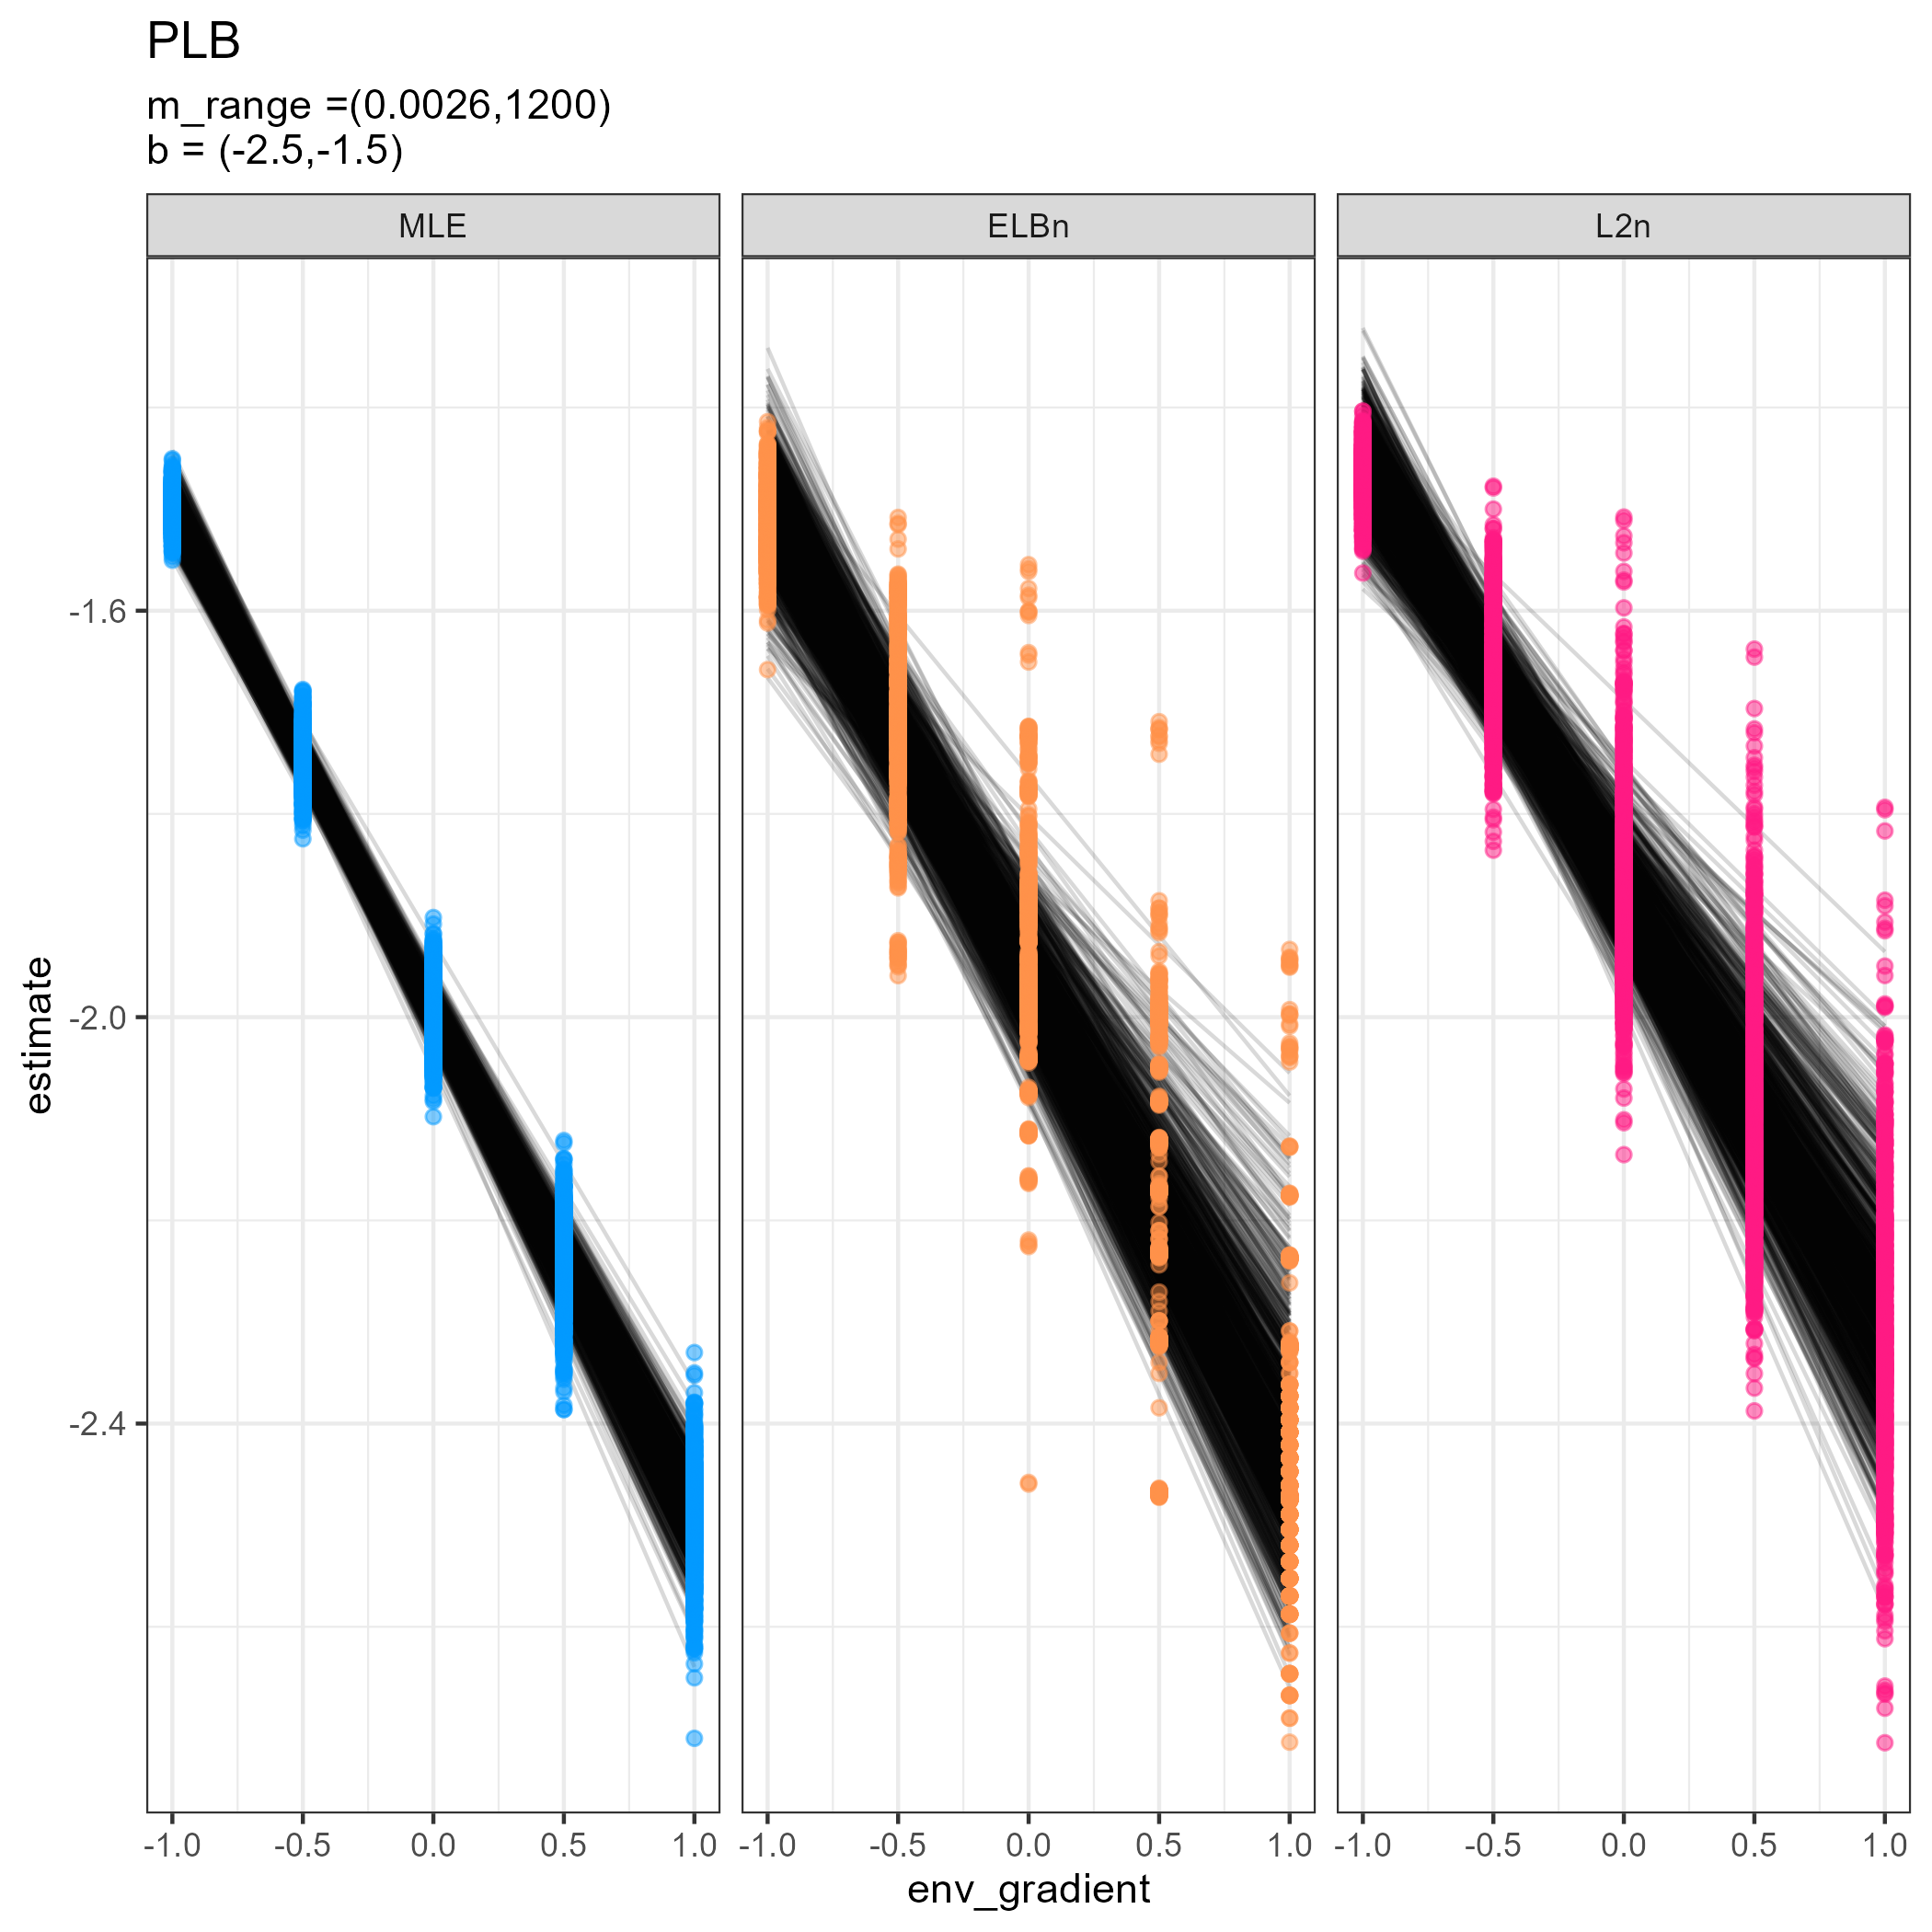
\includegraphics{figures/PLB_sim_main.png}
\caption{Relationship estimates across the hypothetical gradient for
each replicate. Each panel is a different method for estimating the size
spectra parameter.}
\end{figure}

All methods performed reasonably well in detecting the known
relationship across the hypothetical environmental gradient. The
regressions using the MLE method found a significant relationship 100\%
of the time, while the ELBn and NAS method found significant
relatoinships 95.8\% and 96.9\% of the time, respectively.

The confidence intervals for the relationship coefficients (\(\beta_1\))
for both the MLE and ELBn method contained the true value of the known
relationship across the gradient \(\ge\) 95\% of the time, whereas the
confidence interval for the NAS method only had the true value 83.1\% of
the time. Despite having similar accuracy, the width of the CIs for the
ELBn method were more than 3 times that of the MLE method (ELBn\_CI\_ =
0.386 \(\pm\) 0.20; MLE\_CI\_ = 0.121 \(\pm\) 0.056). The CI's for the
NAS were slightly smaller than the ELBn method, but still \(>\) 2.5
times as wide as the MLE method (NAS\_CI = 0.339 \(\pm\) 0.172).

On average, the relationship across the gradient was under estimated:
MLE -0.002 (\(\pm\) 0.022); ELBn -0.039 (\(\pm\) 0.062); and NA -0.081
(\(\pm\) 0.061).

\begin{figure}
\centering
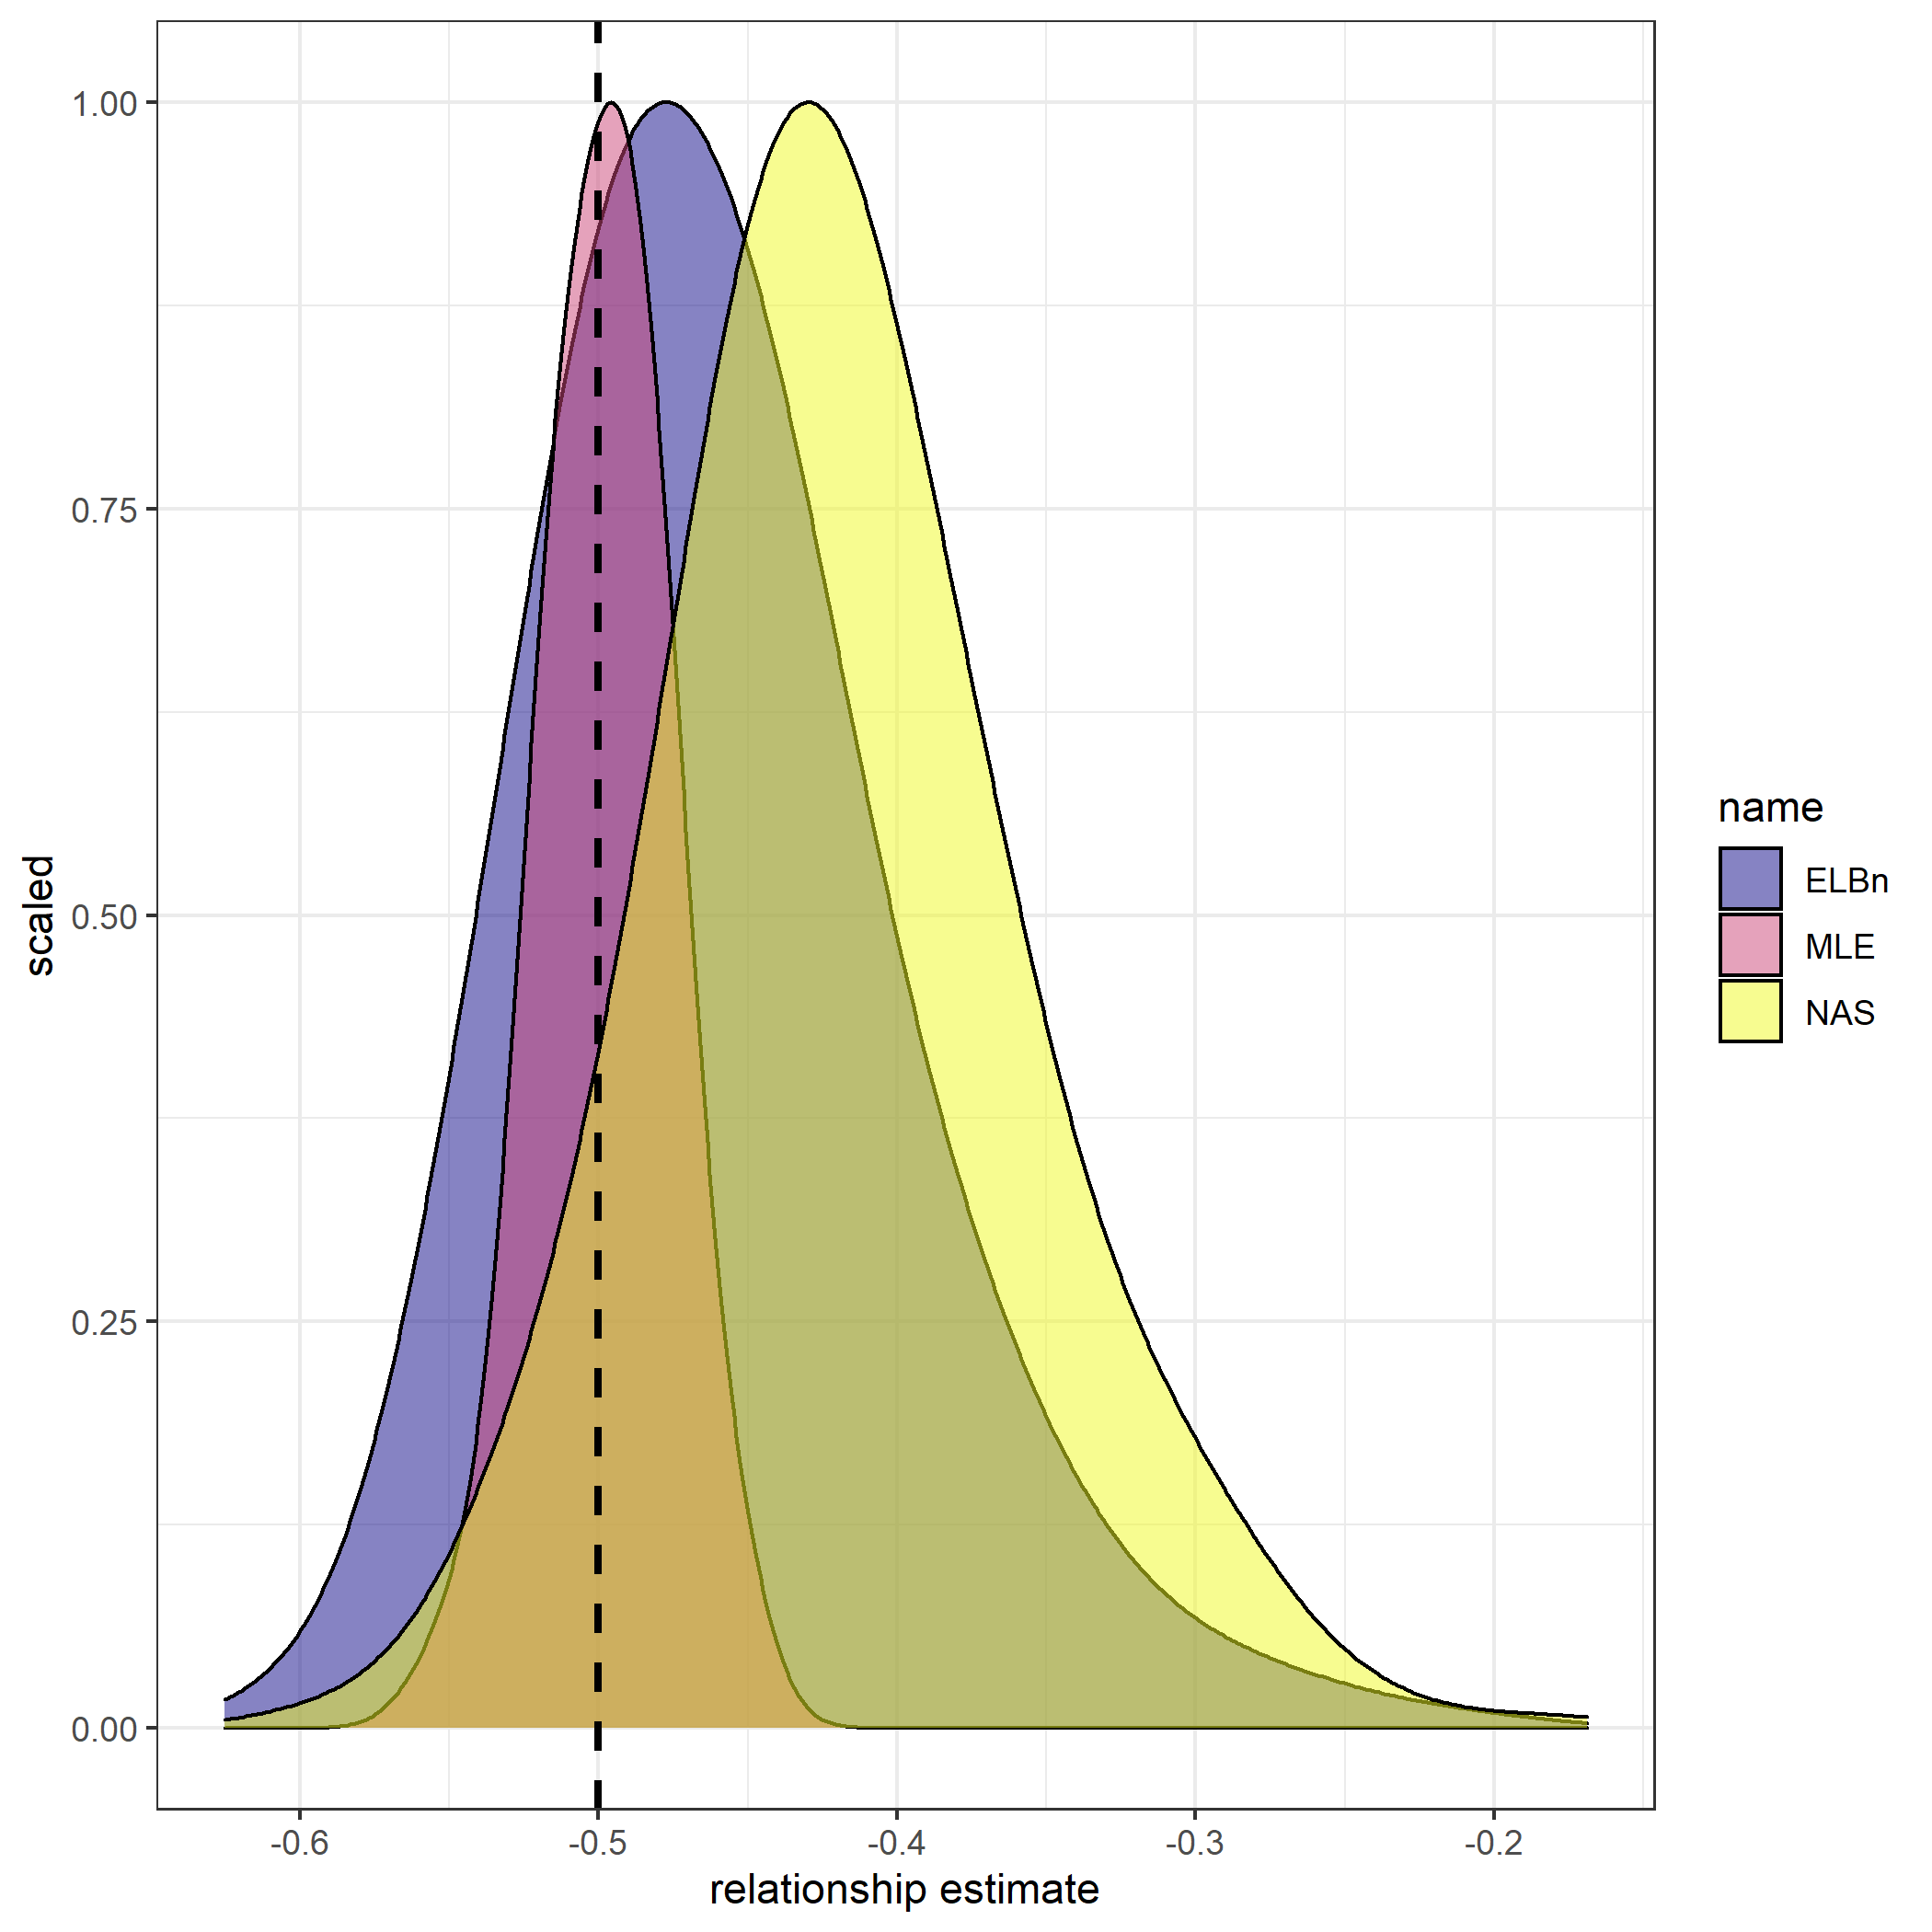
\includegraphics{figures/PLB_sim_relationship_density.png}
\caption{Distribution of relationship coefficient estimates. Vertical
line is the known relationship. All methods under estimate the value,
but the mean magnitude and distribution of values is greater for the
ELBn and NAS methods.}
\end{figure}

Interestingly, there was an interactive effect of the estimate accuracy
between sample size and the value of \(\lambda\). All methods were more
accurate with larger sample sizes, and smaller values of \(\lambda\).

\begin{figure}
\centering
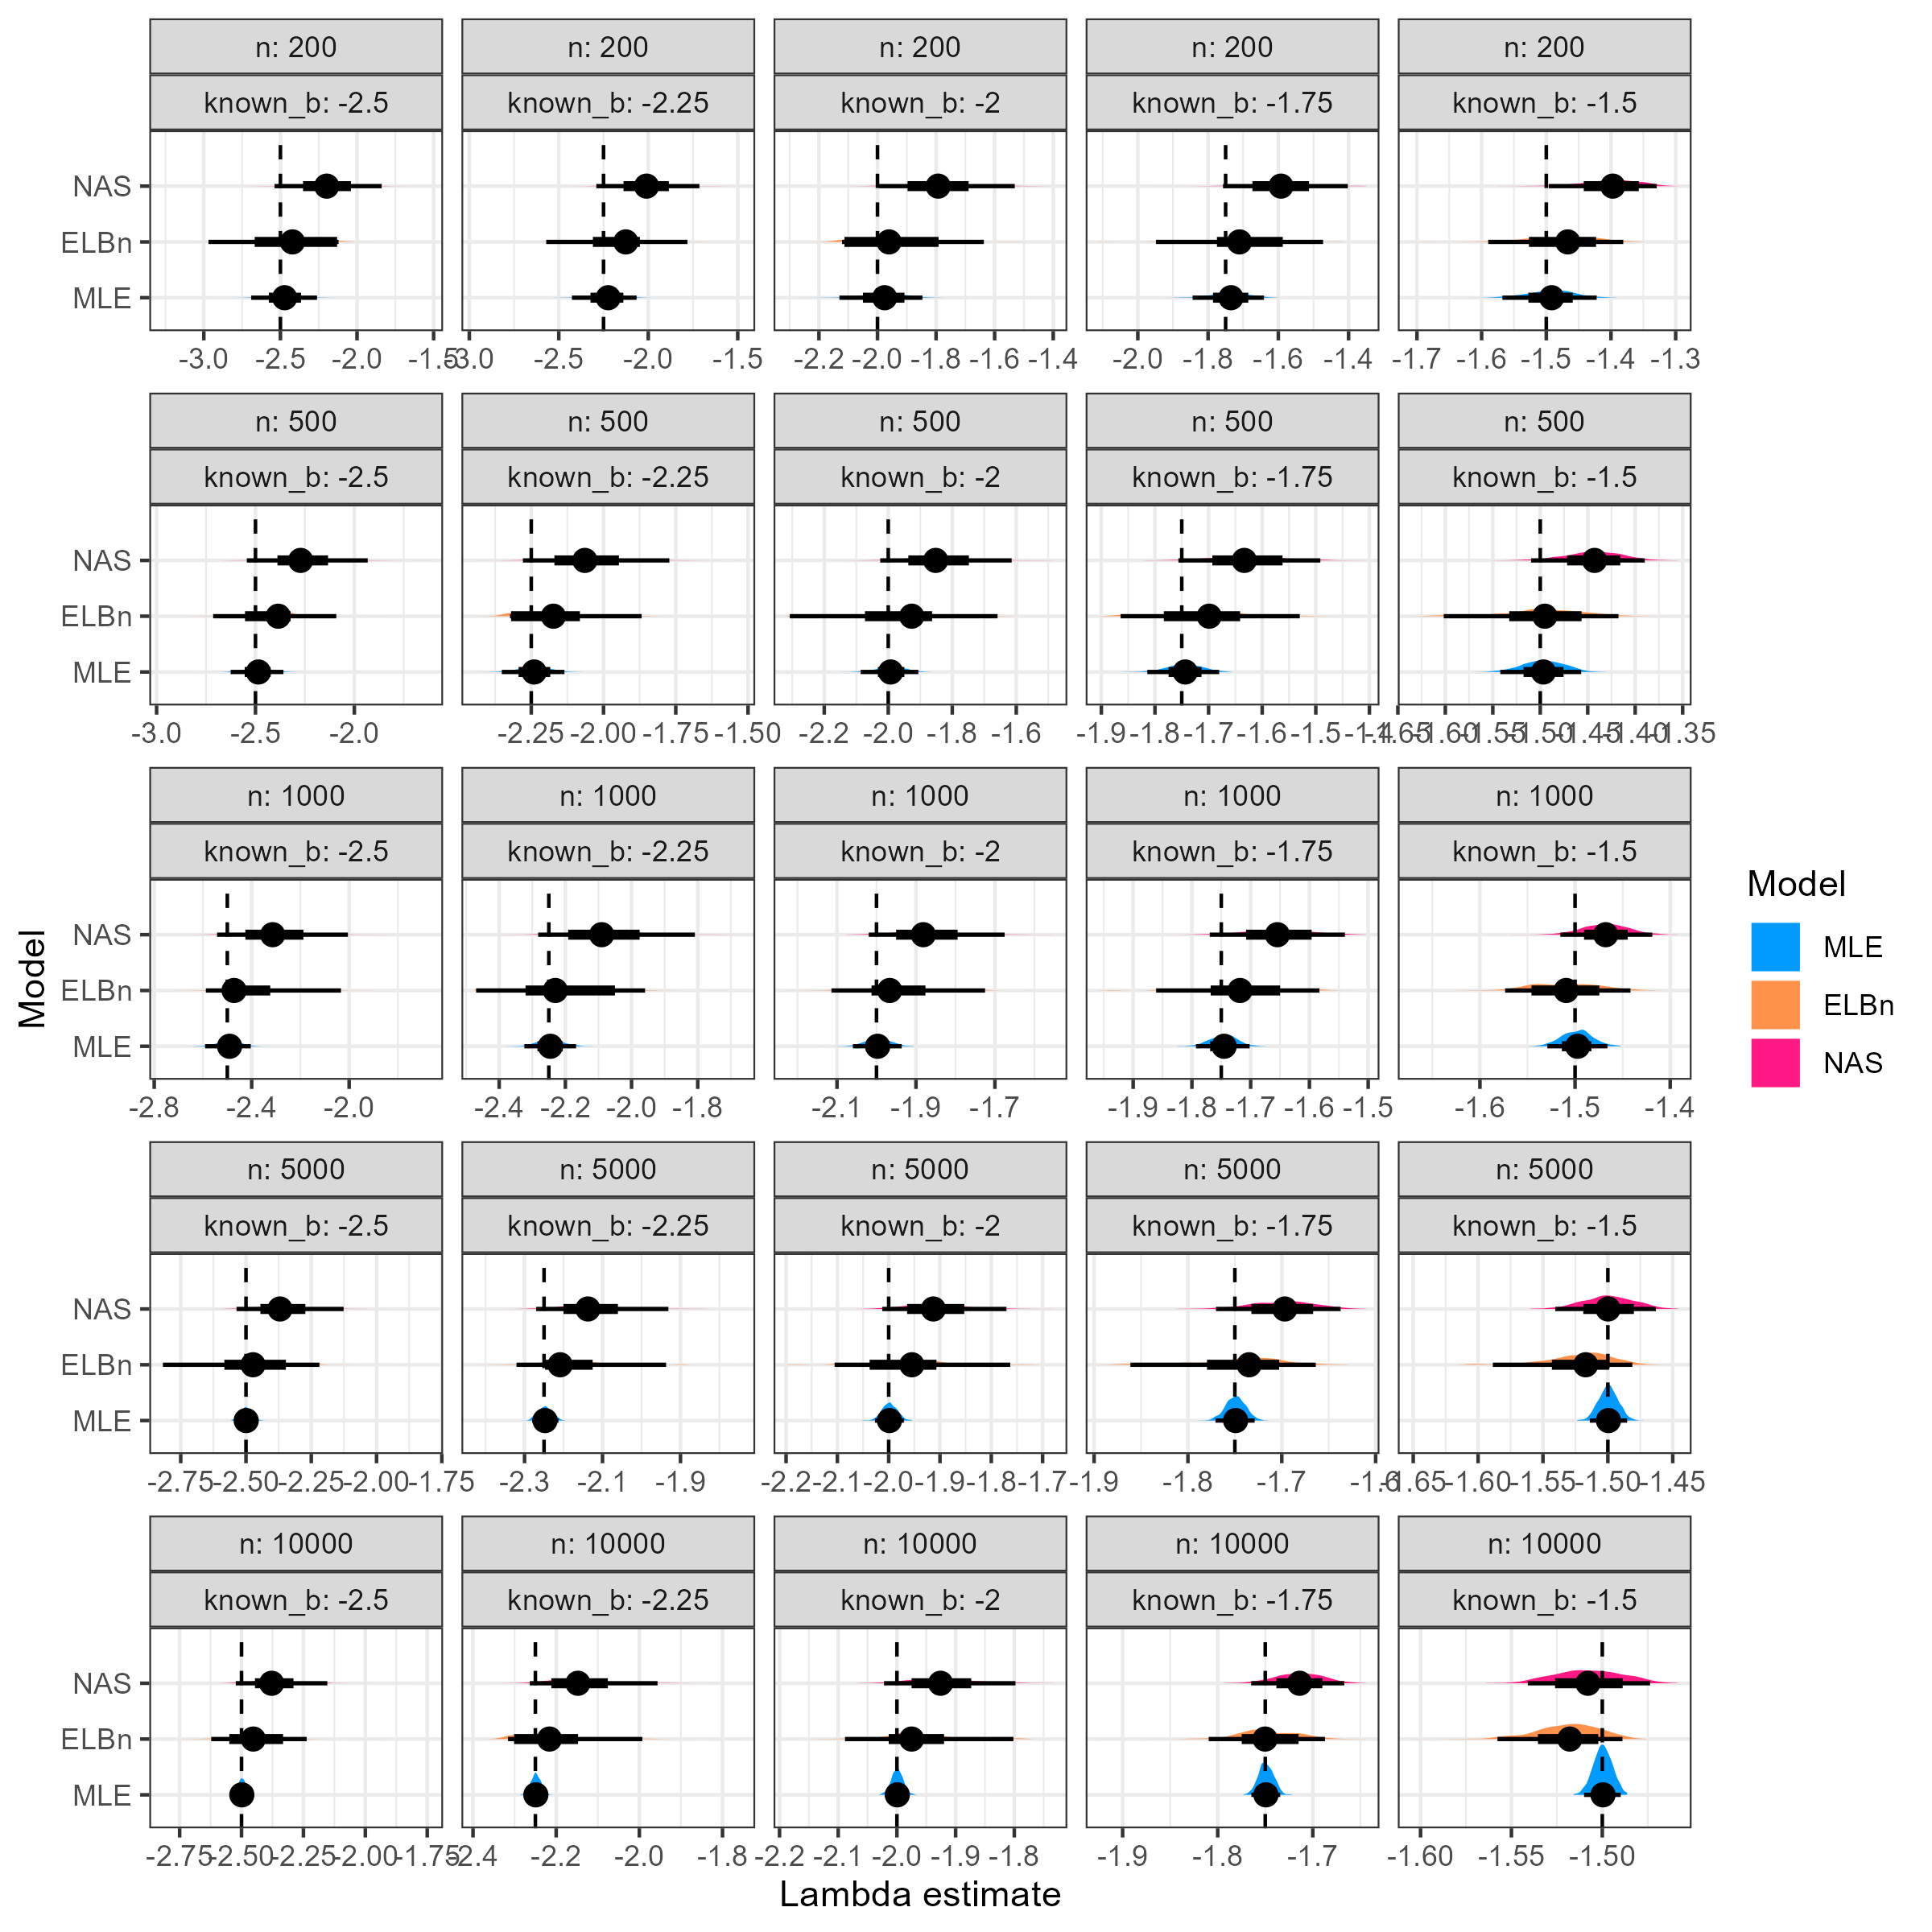
\includegraphics{figures/n_vary_est_b.png}
\caption{Distribution of size spectra parameter estimates. Vertical line
is the known parameter wich describes the bounded power law distribution
from which the body size estimates were sampled. As n increases (top to
bottom) and \(\lambda\) increases (left to right), the accuracy of the
estimate improves across all methods.}
\end{figure}

\begin{figure}
\centering
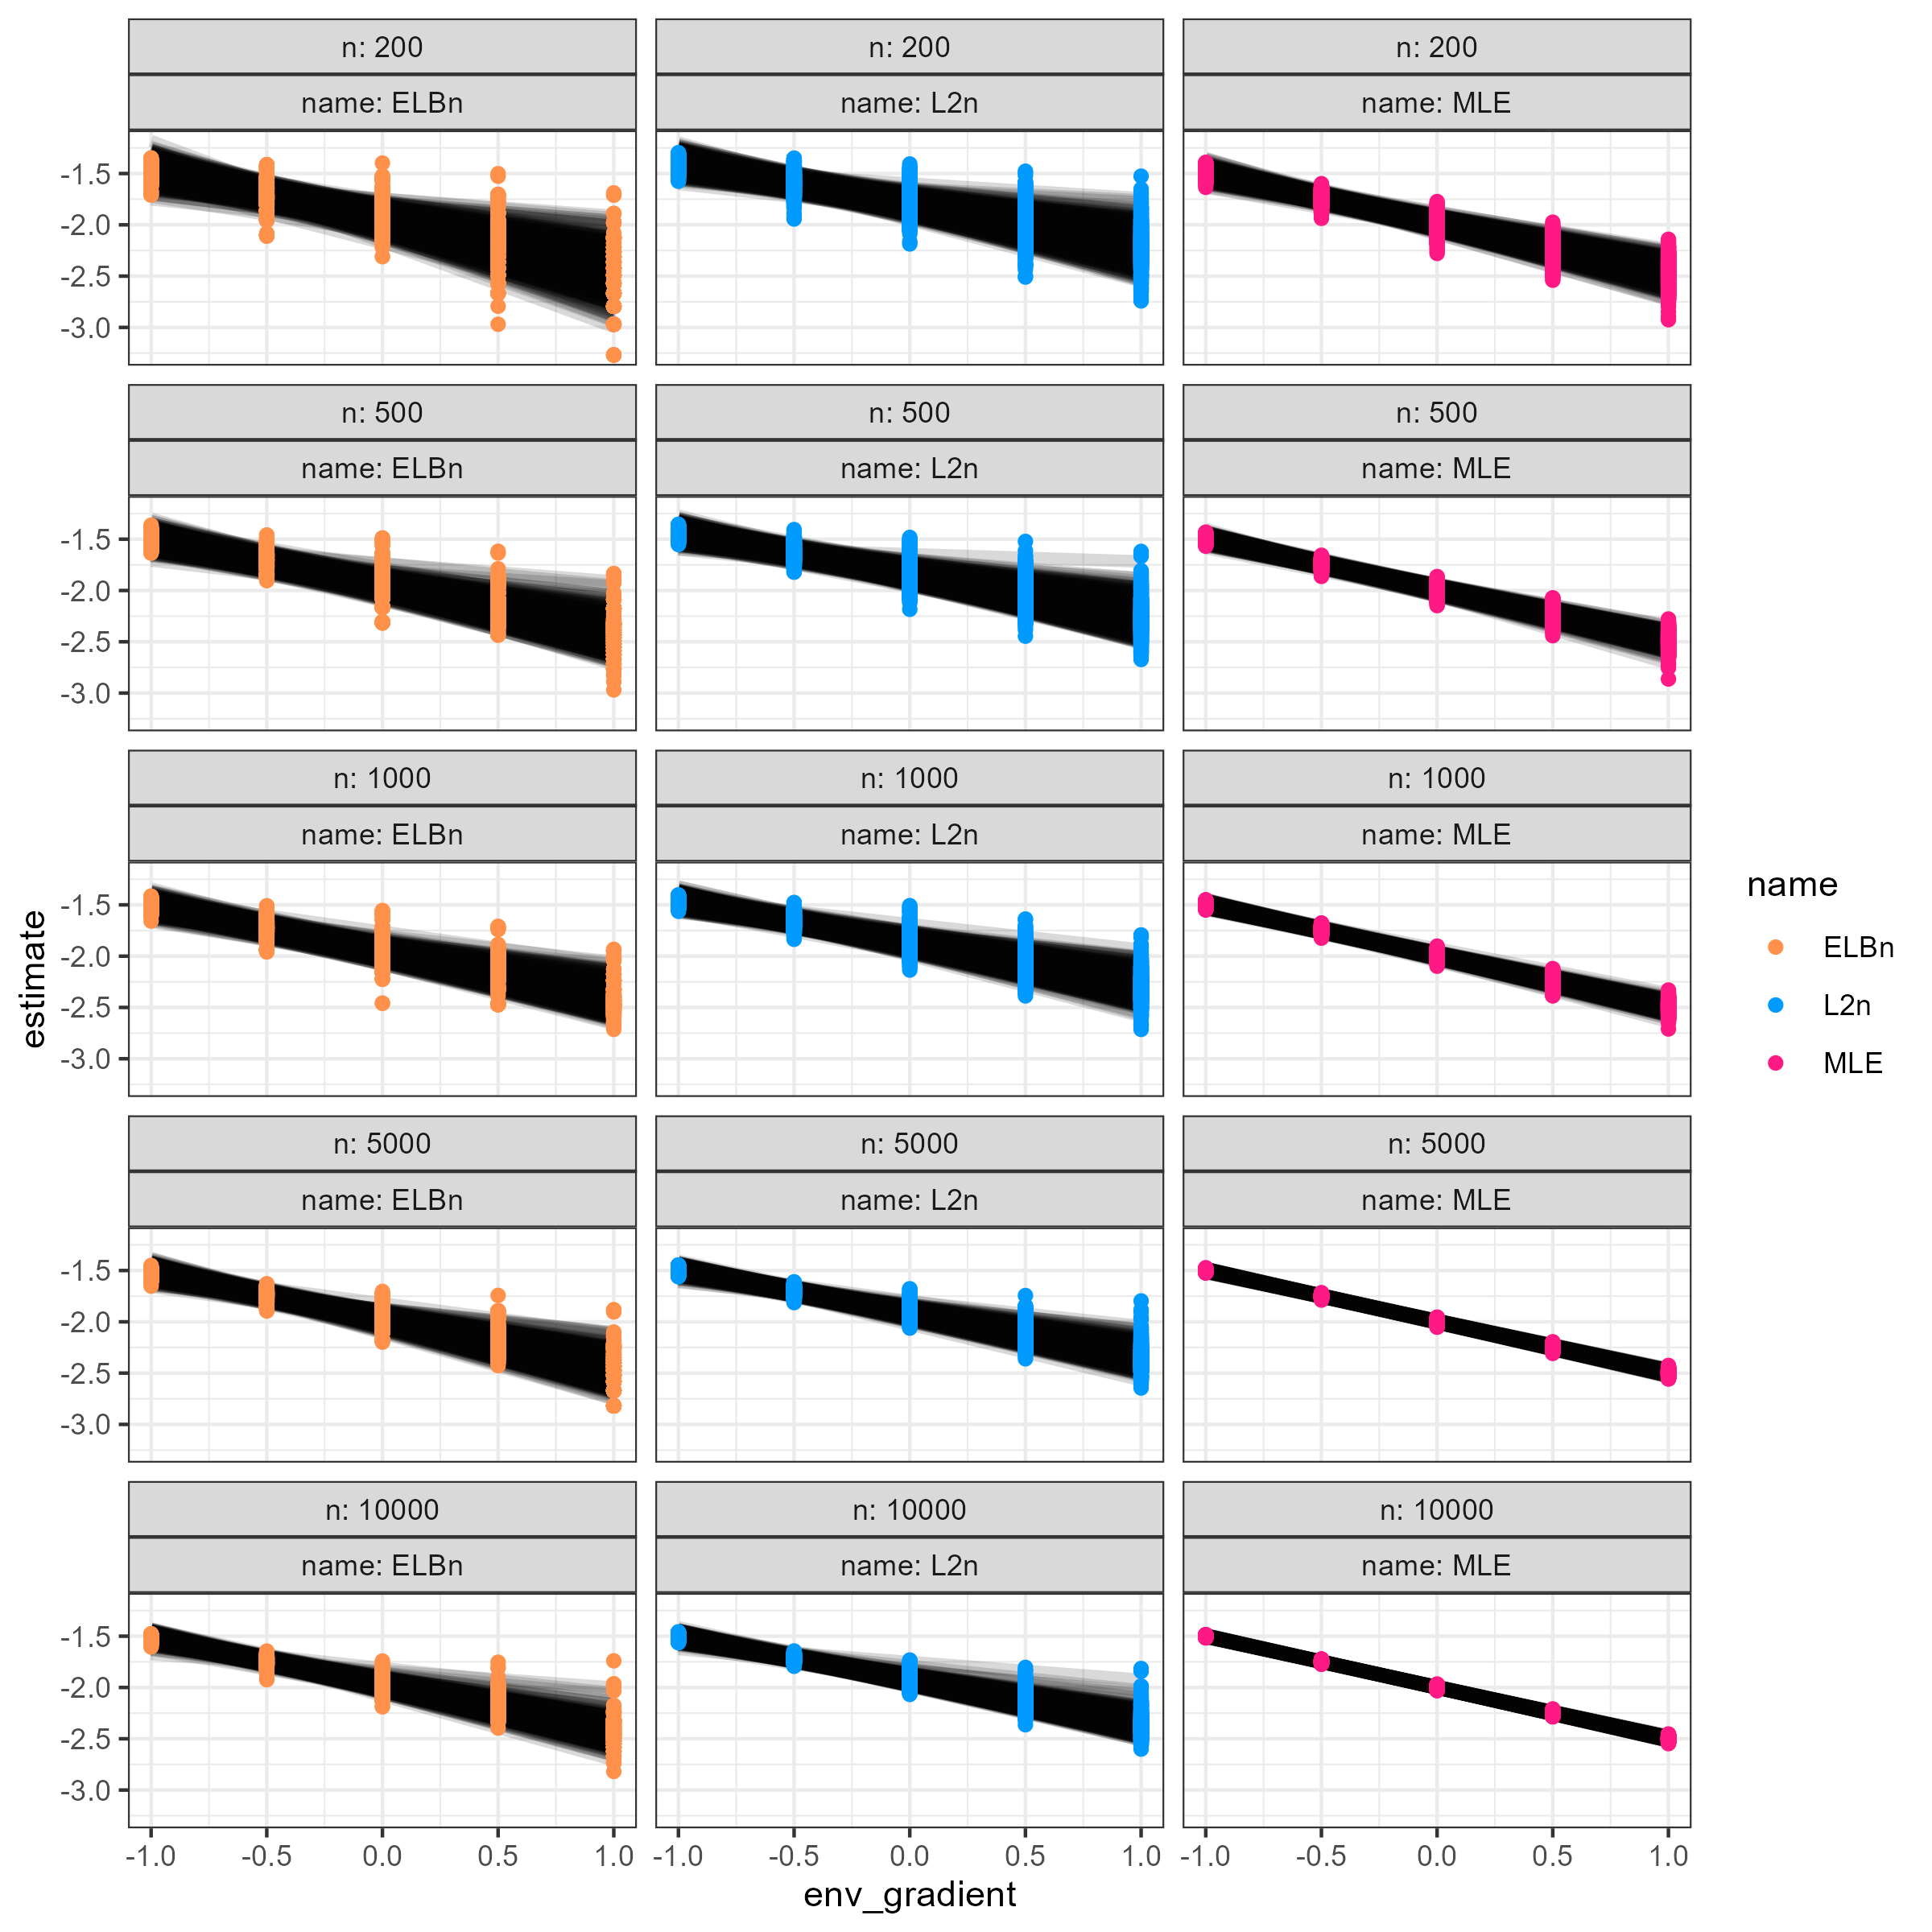
\includegraphics{figures/n_vary_main.png}
\caption{Individual regression estimates across the hypothetical
gradient based on sample size (rows) and methodology used (columns).}
\end{figure}

\hypertarget{no-relationship-1}{%
\subsection{No relationship}\label{no-relationship-1}}

All of the methods performed similarly when there was no relationship
across the hypothetical gradient. The Type I error rate for MLE, ELBn
and NAS were 5\%, 5.7\% and 4.6\%, respectively. However, the confidence
intervals for the binning methods were \textasciitilde3 times as wide as
the MLE method (mean CI widths: MLE = 0.116, ELBn = 0.372; NAS = 0.332).

Of the relationships which were estimated to be significant, the MLE,
ELBn, and NAS method had a 58\%, 49.1\% and 54.3\% probability of
indicating a negative relationship, respectively.

\begin{figure}
\centering
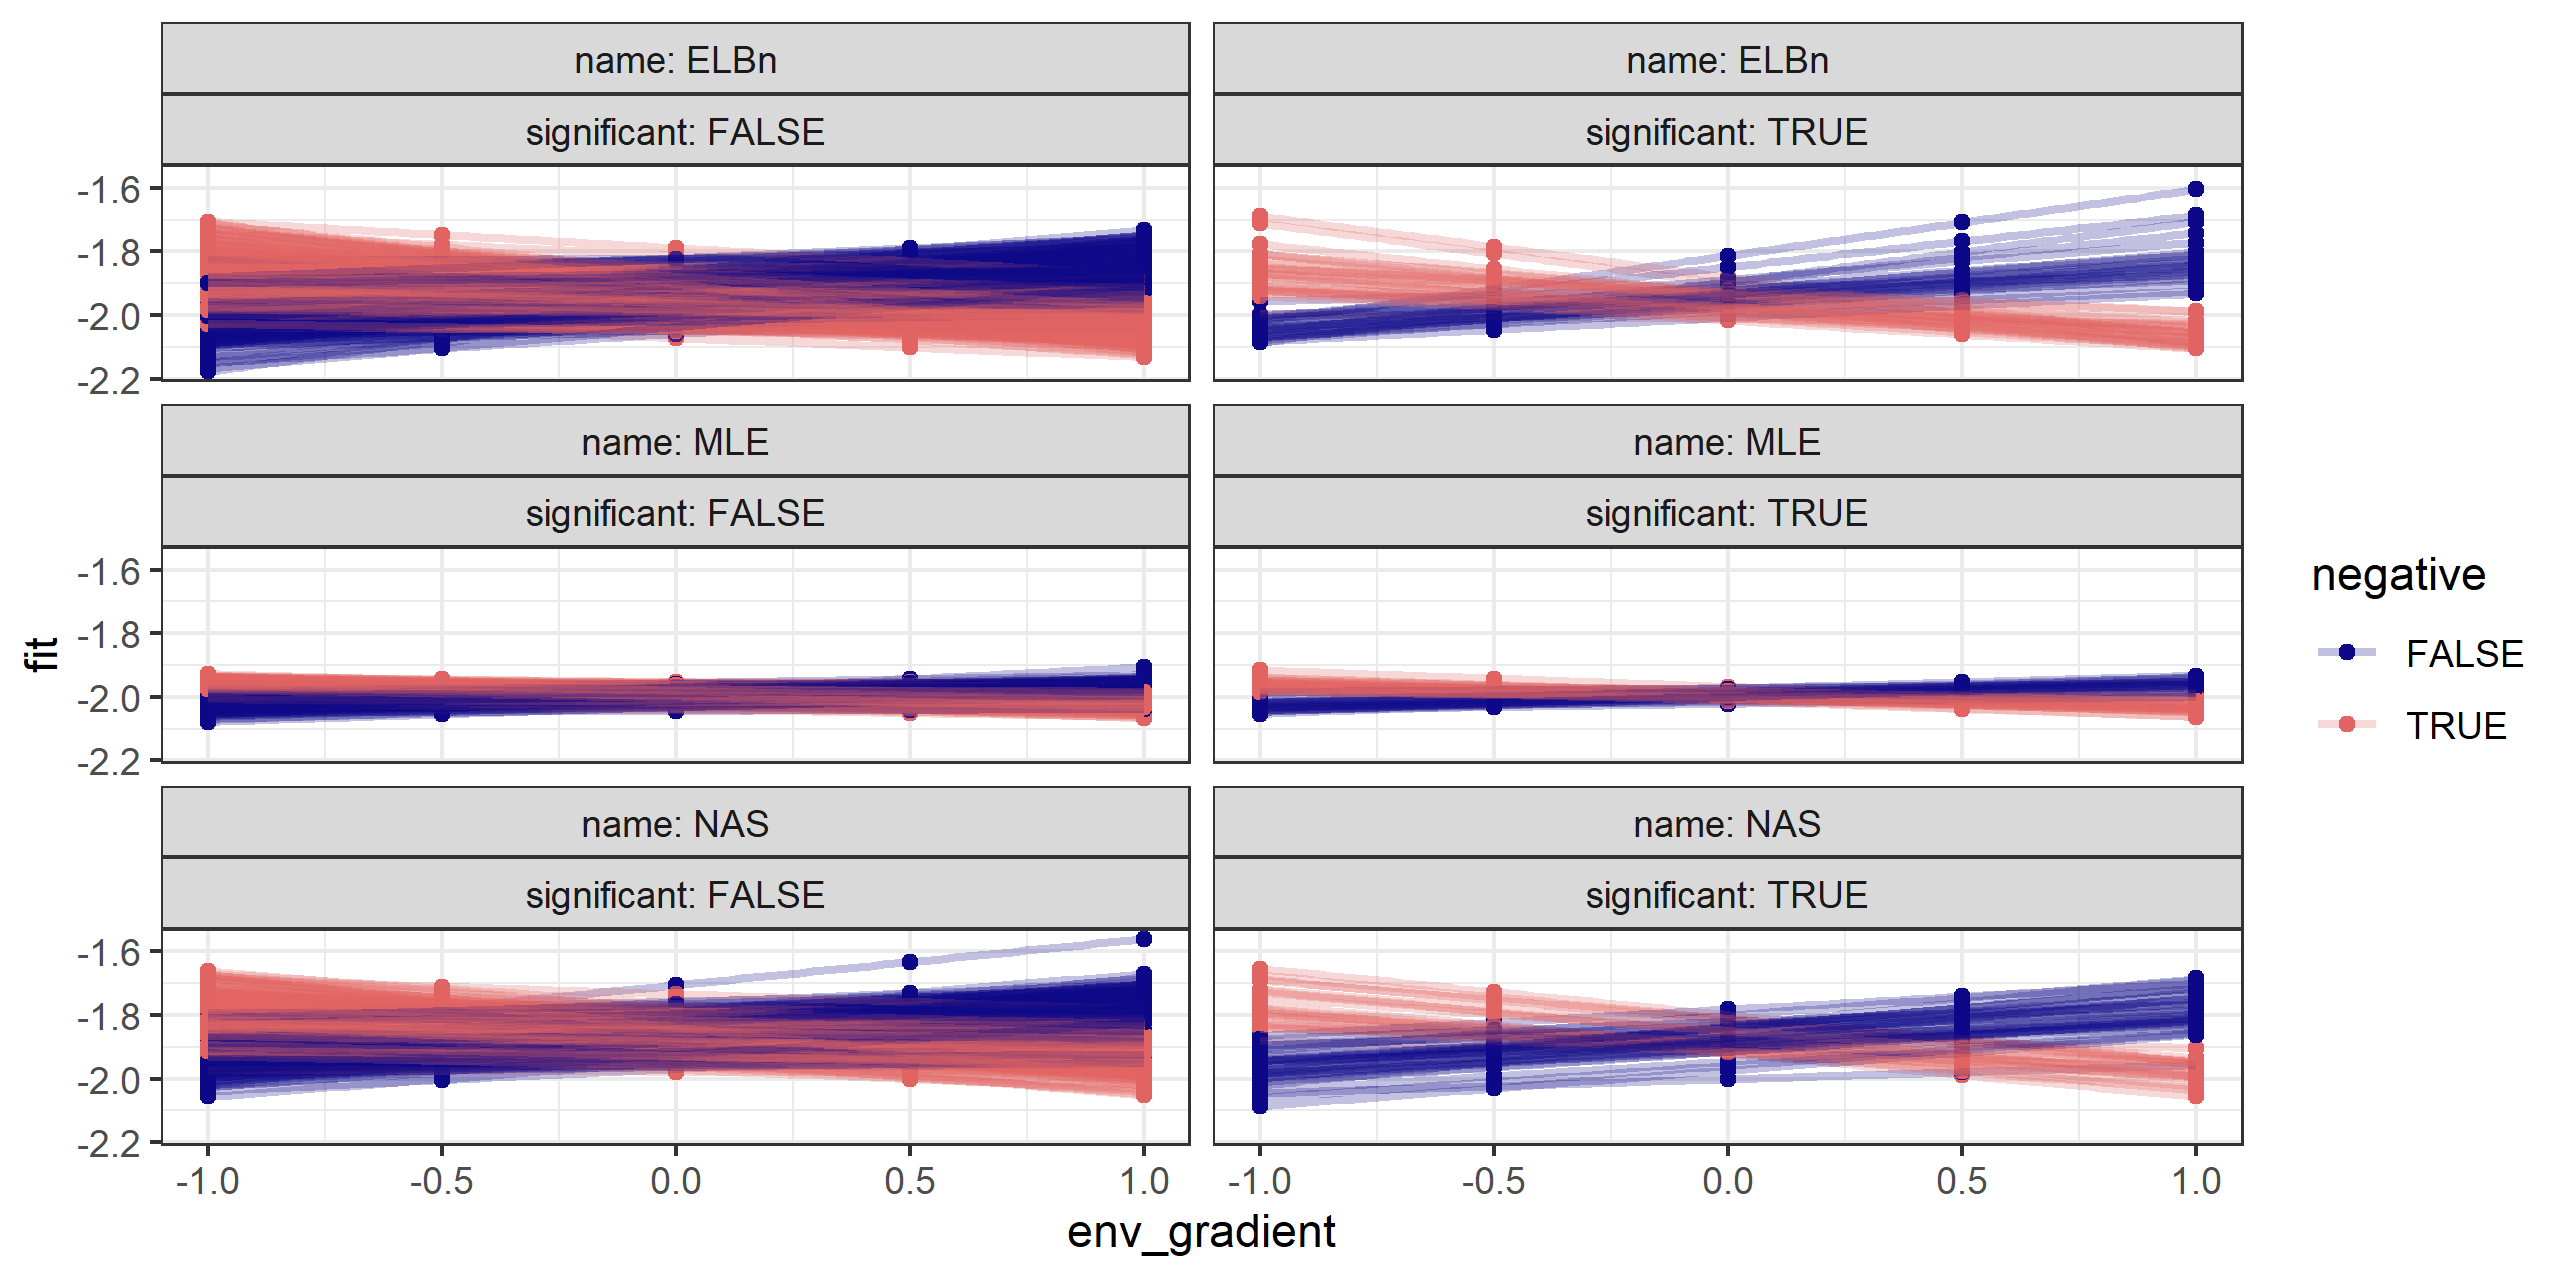
\includegraphics{figures/static_b_lambda_spaghetti.png}
\caption{Individual regression estimates when no relationship exists
across the hypothetical environmental gradient. The methods are
separated by rows, and the left and right column show relationships
which were non-significant and significant, respectively. The individual
regressions coefficients are colored-coded to indicate positive and
negative relationship estimates.}
\end{figure}

\hypertarget{small-variation-in-lambda}{%
\subsection{Small variation in lambda}\label{small-variation-in-lambda}}

The performance of all methods declined when trying to detect variation
in the \(\lambda\) parameter between -1.9 to -2.1 across the
environmental gradient. The mean \(\beta_1\) coefficient estimates for
all methods were closely associated with the known relationship. Once
again the variation in the estimates using the MLE method were much
smaller that the estimates using both of the binning methods (Figure 4).

\begin{figure}
\centering
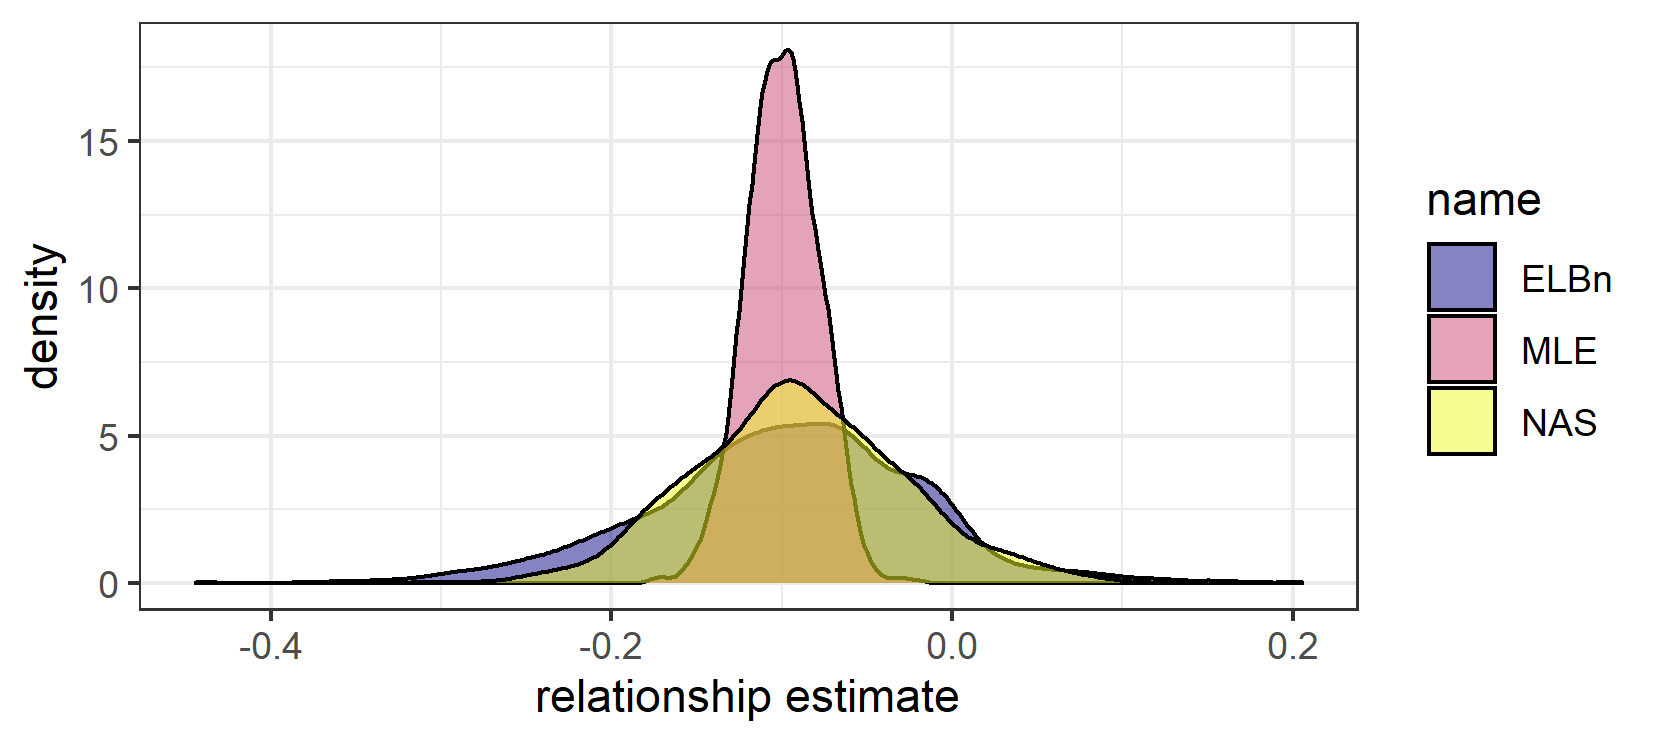
\includegraphics{figures/PLB_sim_small_relationship_density.png}
\caption{Mean difference between relationship estimate and known
relationship coefficient for each method. Here, \(\lambda\) varied from
-1.9 to -2.1, with a kown relationaship of -0.1 across the gradient.}
\end{figure}

Of the 1000 simulation replicates, the MLE only detected a significant
relationship 90\% of the time, whereas the ELBn and NAS methods detected
significant relationships 19 and 23\% of the time, respectively. Of the
replicates which were significant, the confidence interval contained the
true value of the relationship 94.6, 88.4, and 89.1\% of the time for
the MLE, ELBn, and NAS methods, respectively.

\begin{figure}
\centering
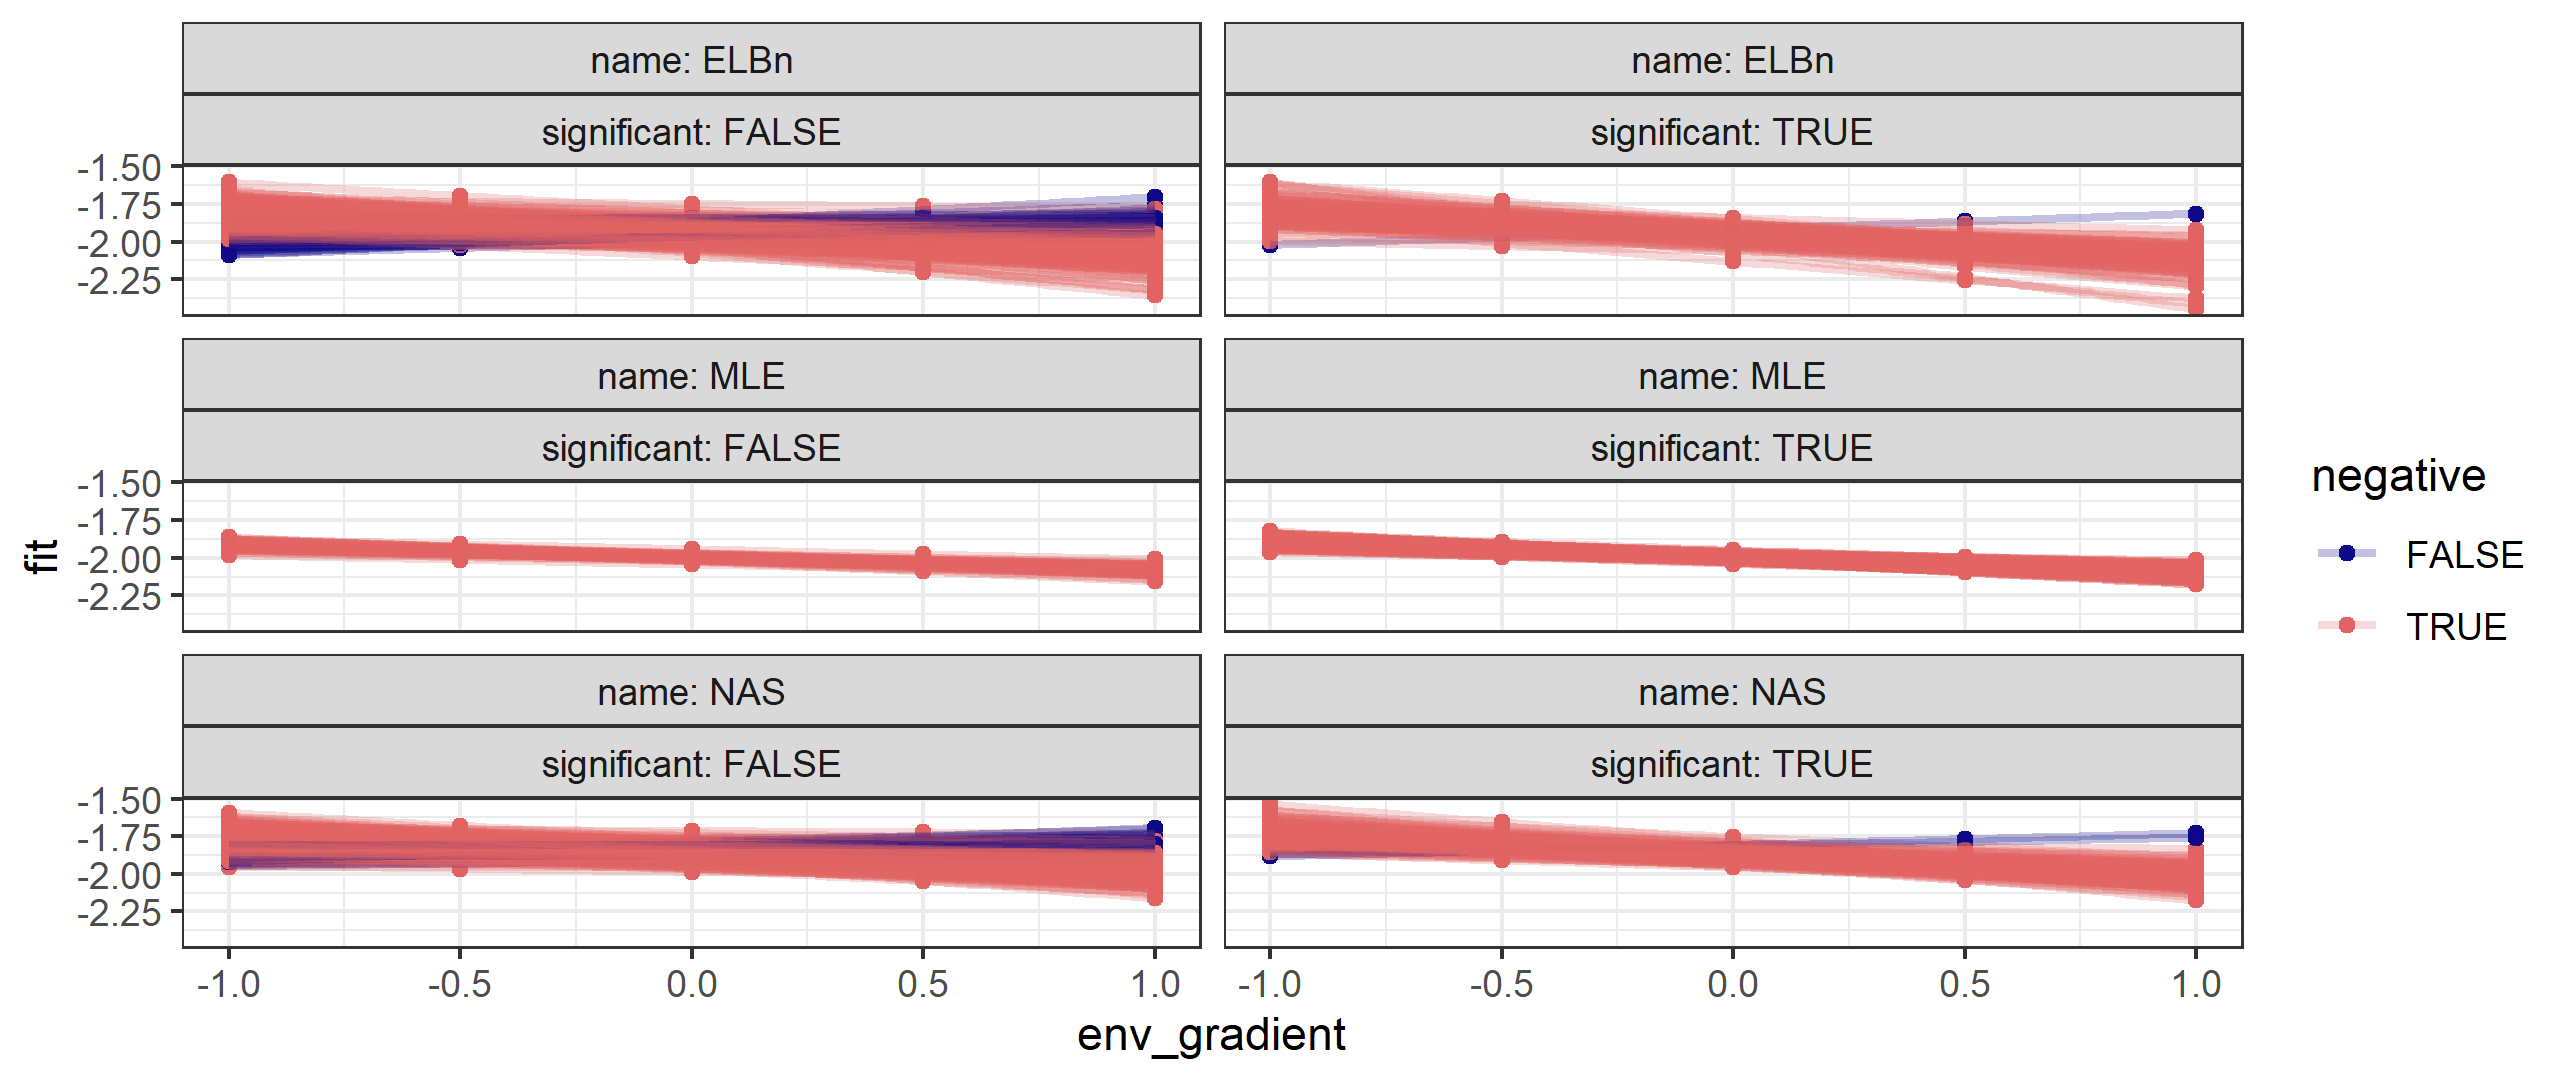
\includegraphics{figures/small_lambda_spaghetti.png}
\caption{Linear regressions across the hypothetical gradient when lambda
varies from -1.9 to -2.1. Each method is displayed in the rows, and the
left colum shows the non-significant estimates, while the right column
shows the relationships which were signficant (\(\beta_1\) coefficient
p-value \textless{} 0.05). The colors indicate when the beta coefficient
estimate was negative (pink) and when it was positive (purple).}
\end{figure}

Once again, the width of the confidence intervals for both of the
binning methods were \(\ge\) 2.8 times that of the MLE method (mean
\(\pm\) SD MLE CI width: 0.117 \(\pm\) 0.051; ELBn CI width: 0.378
\(\pm\) 0.169; NAS CI width: 0.332 \(\pm\) 0.150).

On average, the relationship estimates across the gradient were similar
to the know value (mean deviation: MLE = 0.00001, ELBn = -0.009, NAS =
-0.012). However, when only looking at the relationships which were
significant, this variation increased considerably(MLE = -0.002, ELBN =
-0.052, NAS = 0.034).

\hypertarget{empirical-data-1}{%
\subsection{Empirical data}\label{empirical-data-1}}

For both empirical datasets, the direction and magnitude of chnage
(i.e.~\(\beta_1\) coefficients) are generally in agreement. Size spectra
parameters consistently increase (become flatter) in the AMD data (Fig.
XX A). Likewise, the size spectra parameters consistently increase
(become steeper) with increasing temperature across the NEON sites (Fig
XX D)

\textbf{NOTE} combine all the figures below into one with 4 panels (AMD
= A, B; NEON = C, D)

\begin{figure}
\centering
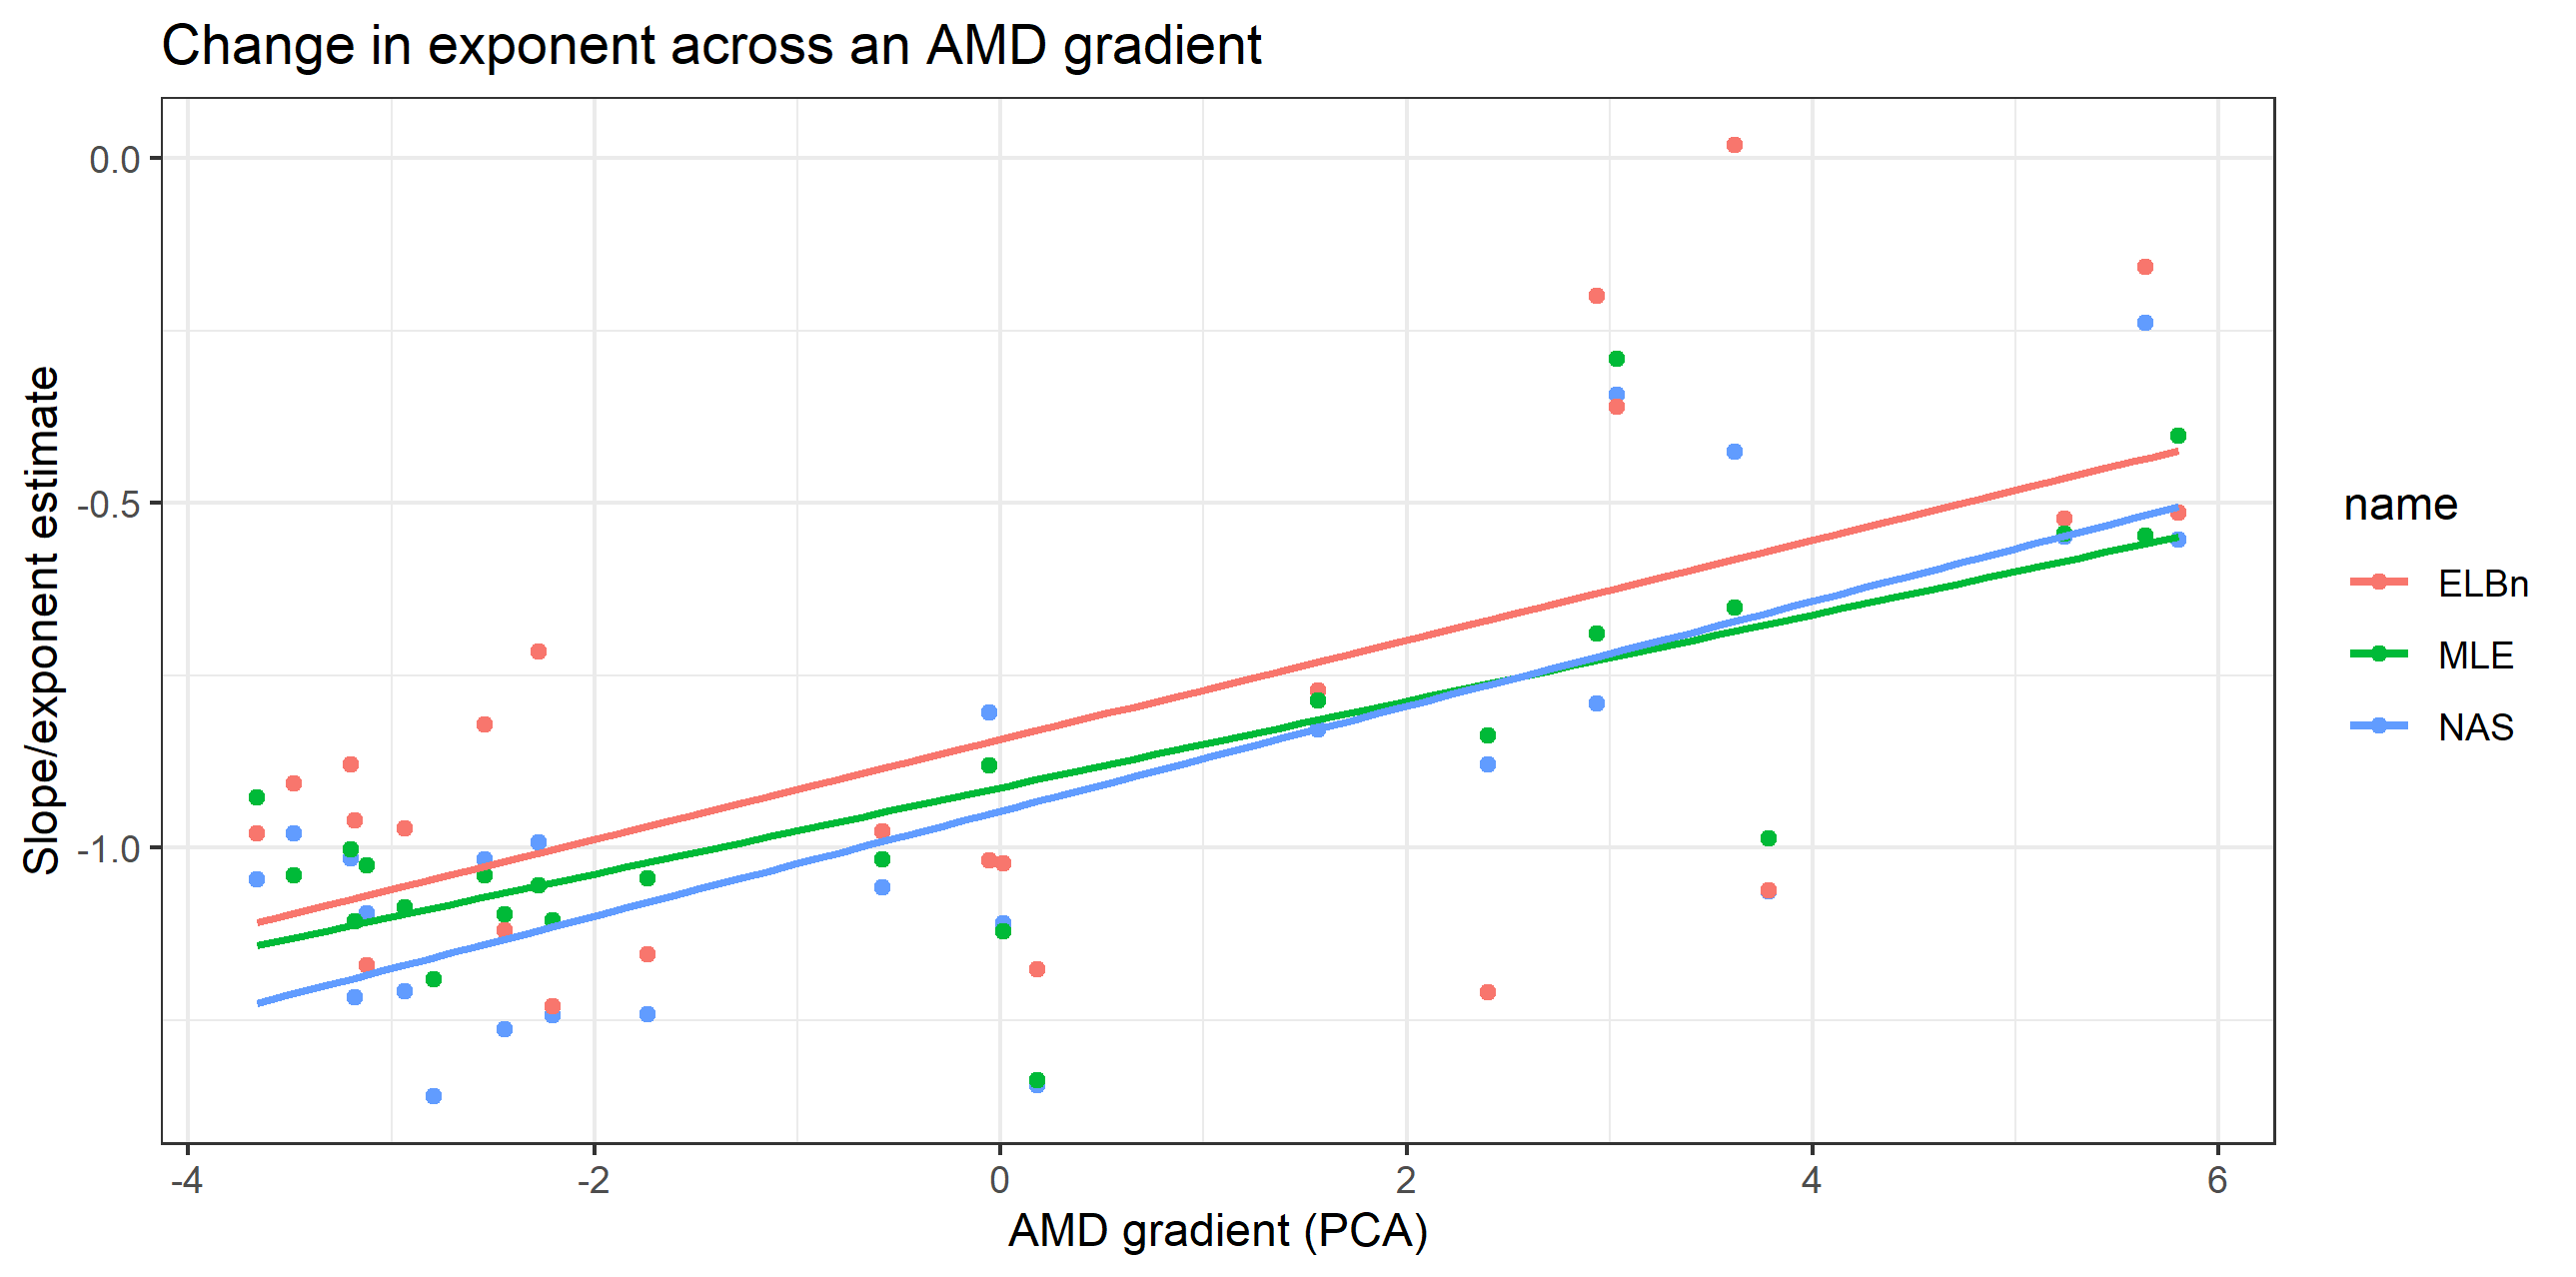
\includegraphics{figures/AMD_plot.png}
\caption{A}
\end{figure}

\begin{figure}
\centering
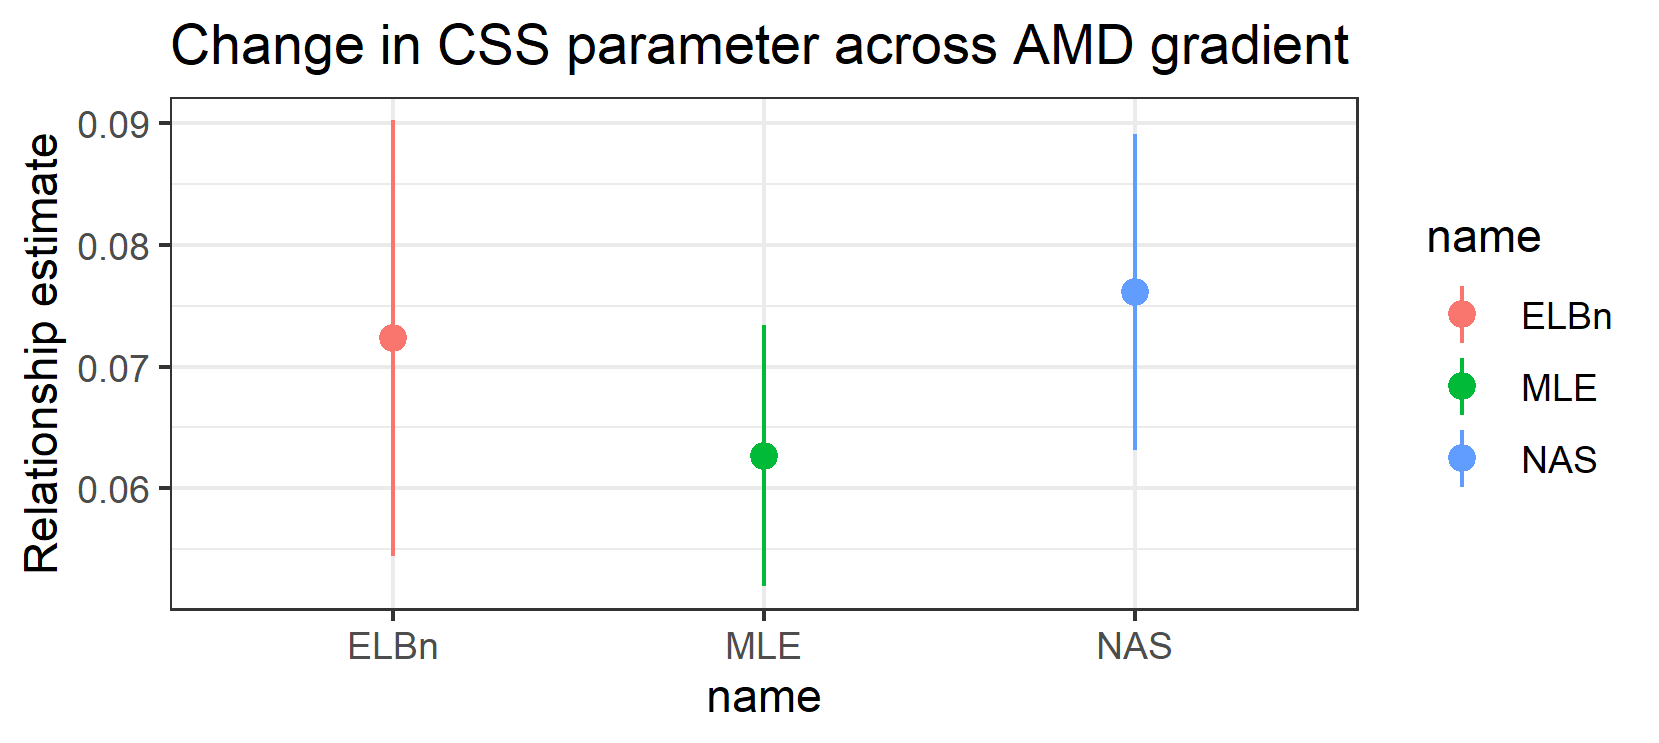
\includegraphics{figures/amd_relationship.png}
\caption{B.Relationship estimates across AMD gradient}
\end{figure}

\begin{figure}
\centering
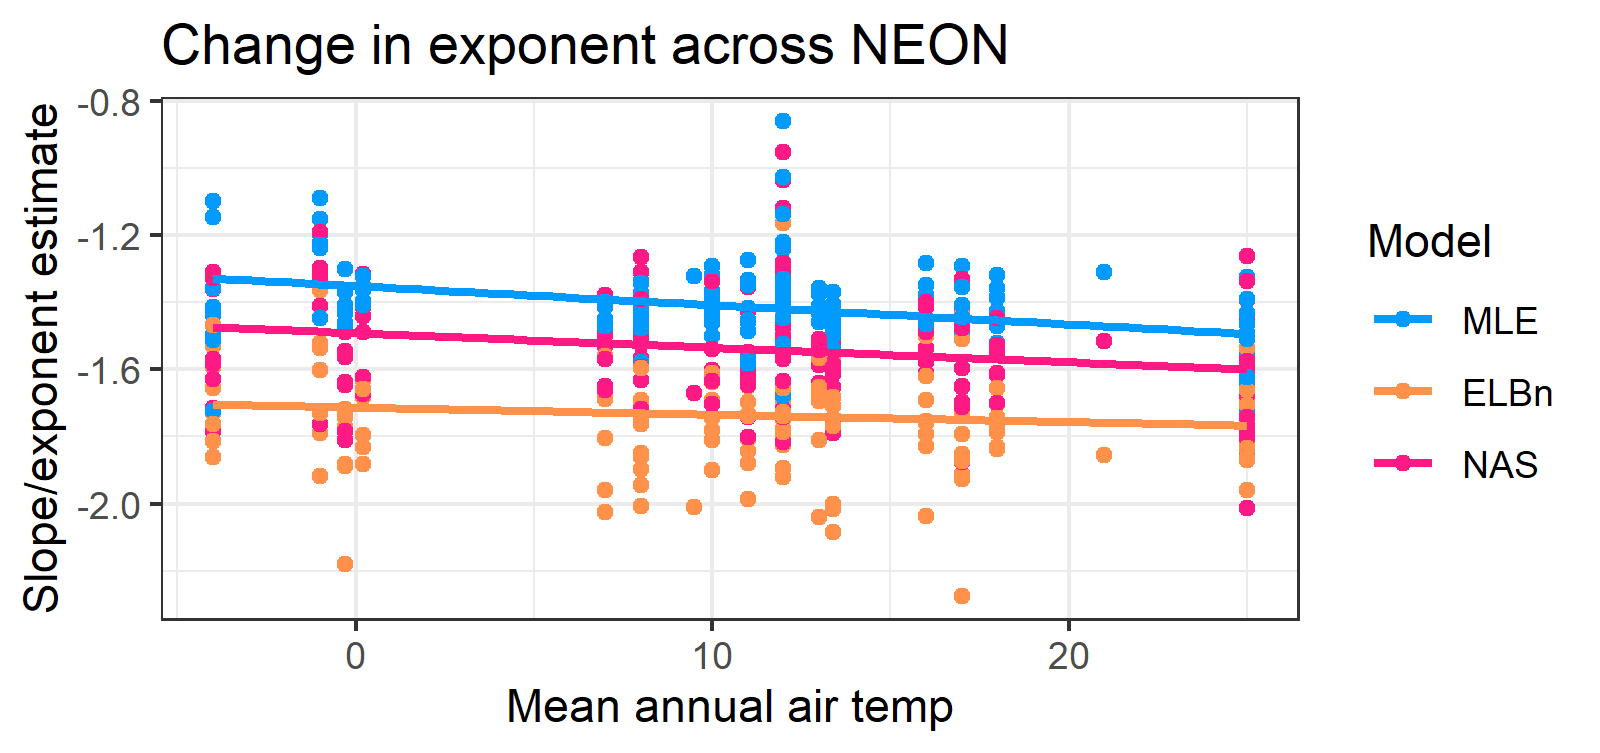
\includegraphics{figures/NEON_plot.png}
\caption{C.}
\end{figure}

\begin{figure}
\centering
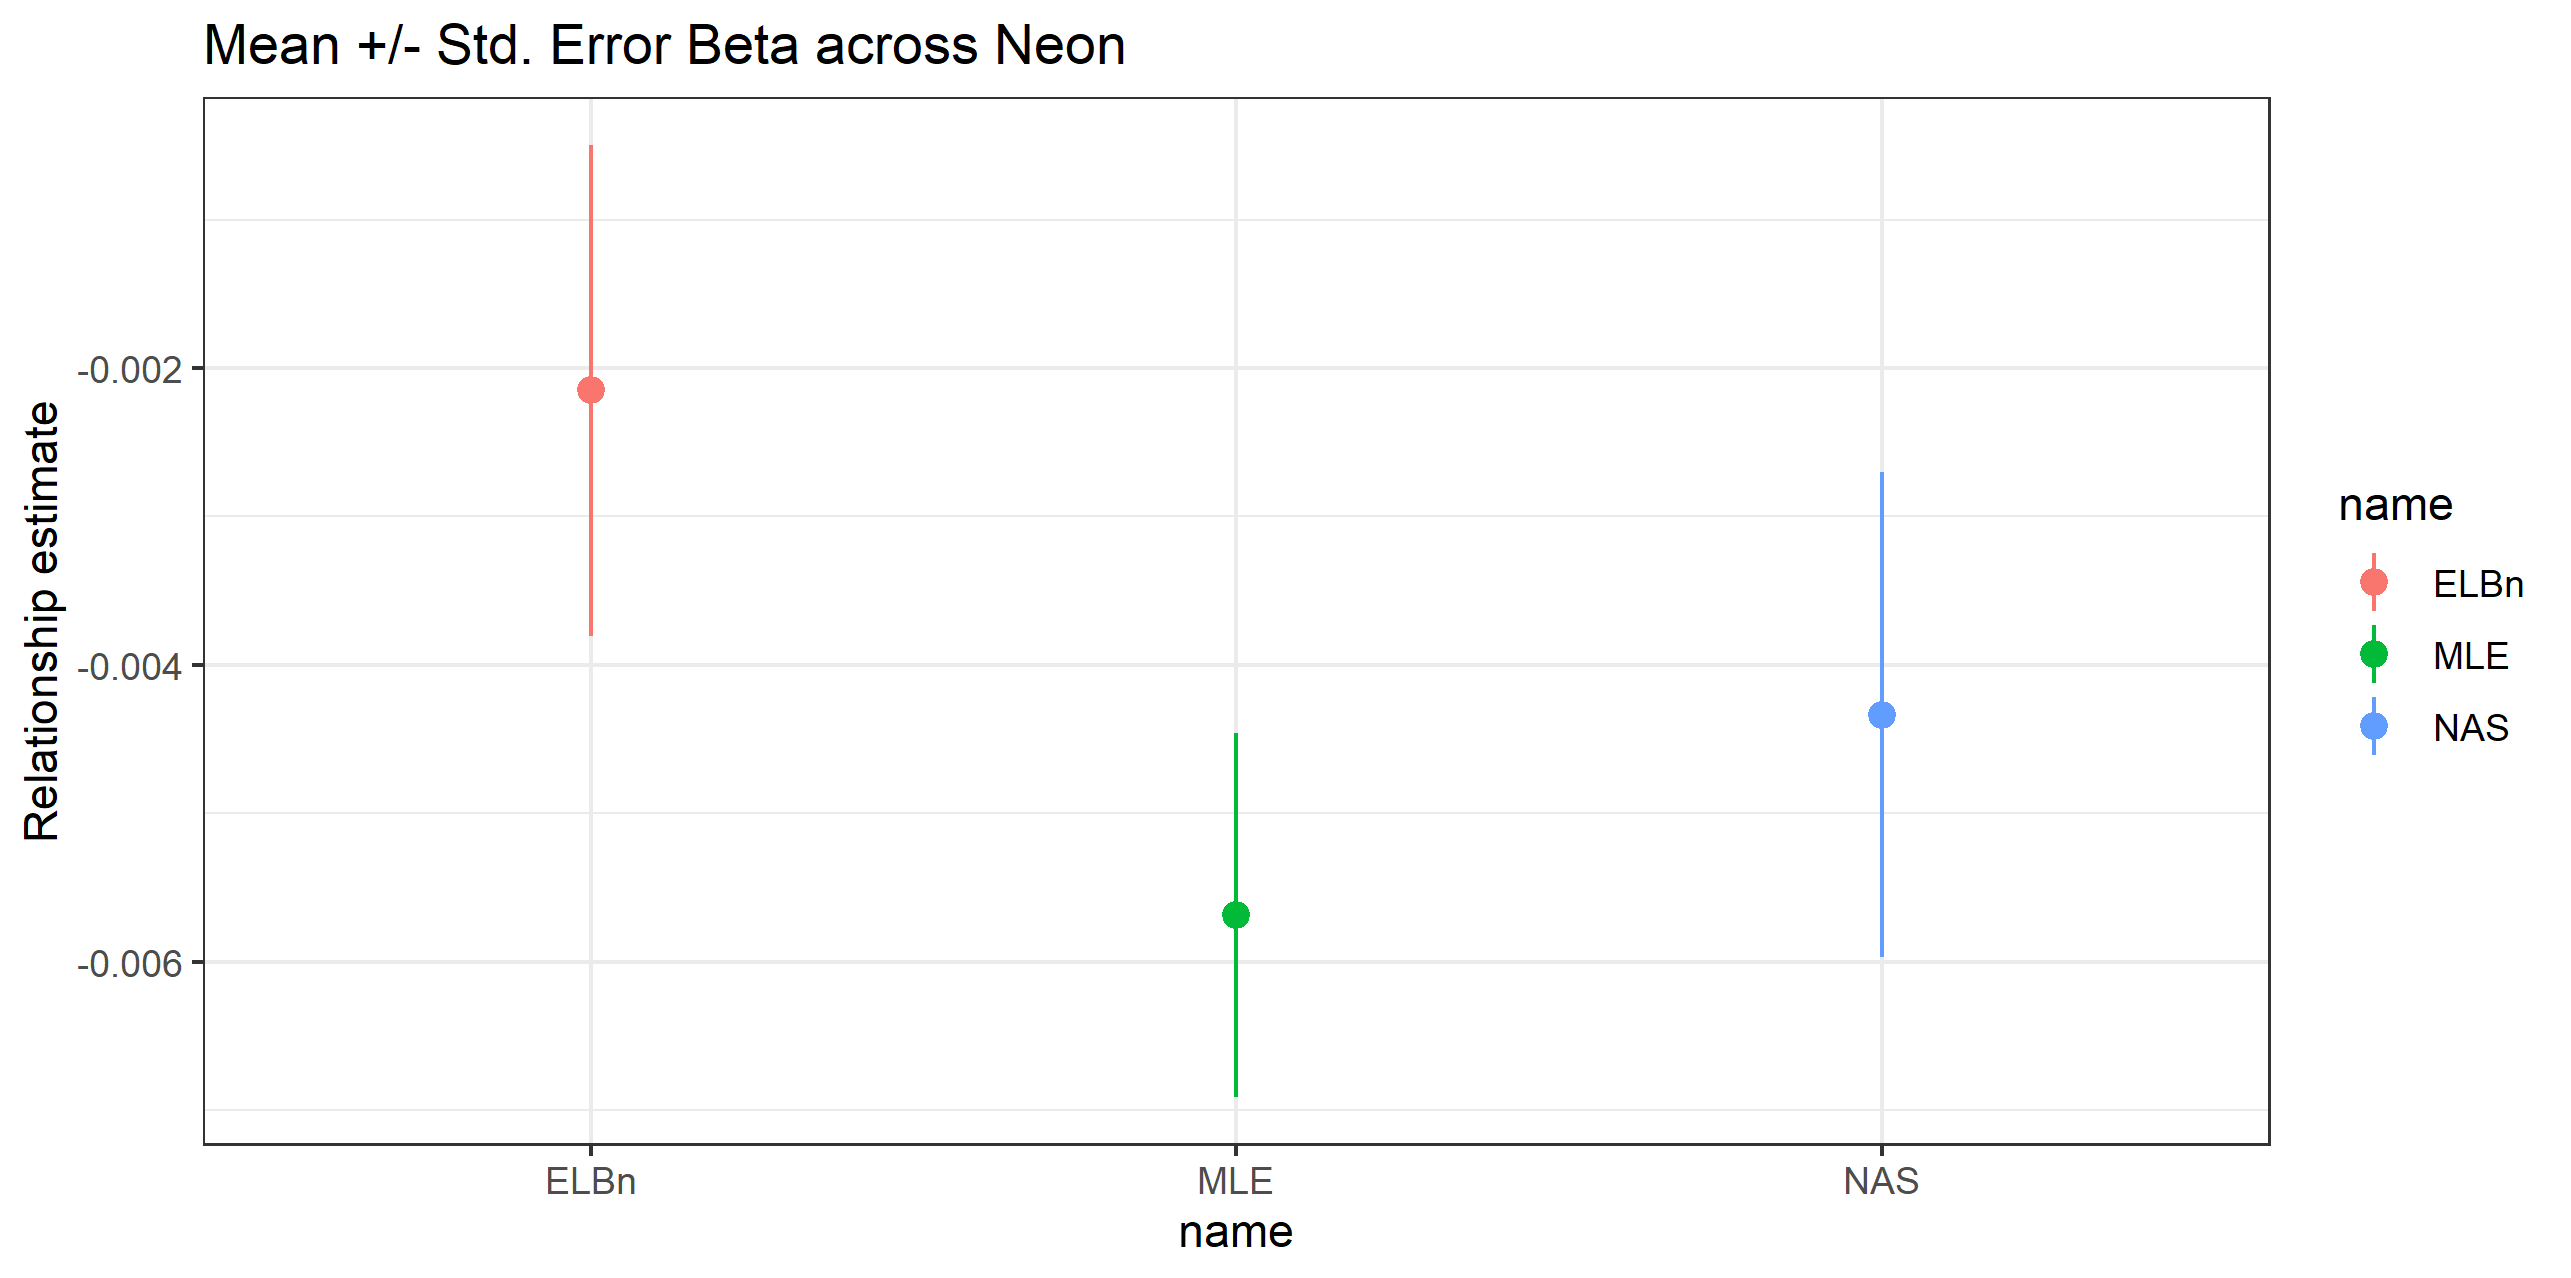
\includegraphics{figures/neon_relationship.png}
\caption{D.}
\end{figure}

Because the \(\beta_1\) coefficient estimates are similar, and the range
of the gradient in the AMD data is relatively small (9.5), the absolute
change in the size spectra parameter across the AMD gradient are similar
regardless of method used (range: 0.59 to 0.72). Likewise, the absolute
change in size spectra parameters across the NEON temperature gradient
ranges from 0.06 to 0.165, depending on the method used.

\emph{alternative} absolute difference of \textasciitilde0.1 units in
\(\lambda\) across gradients is similar to differences reported in other
studies (seasonally: 0.16, Mcgarvey and Kirk; landuse: 0.15 Martinez;
O'Gorman 2017 \textasciitilde0.25, Yvon and Dossena papers
\textasciitilde0.1? {[}need to redownload some of these and
compare{]})(Dossena et al. 2012, O'Gorman et al. 2017, McGarvey and Kirk
2018)

\hypertarget{simulating-shallower-lambdas}{%
\subsection{Simulating shallower
lambdas}\label{simulating-shallower-lambdas}}

Estimates of the relationship between lambda and a hypothetical gradient
varied depending on the method used. However, interpretations of
empirical data were broadly consistent across methodologies. Upon closer
inspection, the values of size spectra parameters in the empirical data
were considerably shallower than -2. Given that we found the performance
of all methods increased with shallower \(\lambda\)'s we wanted to
investigate how the methods performed with simulated values more similar
to the empirical estimates of parameters describing size spectra
relationships. Therefore, we repeated the simulation process as in the
main analysis, but used \(\lambda\) values ranging from -1.1 to -1.5.

\begin{figure}
\centering
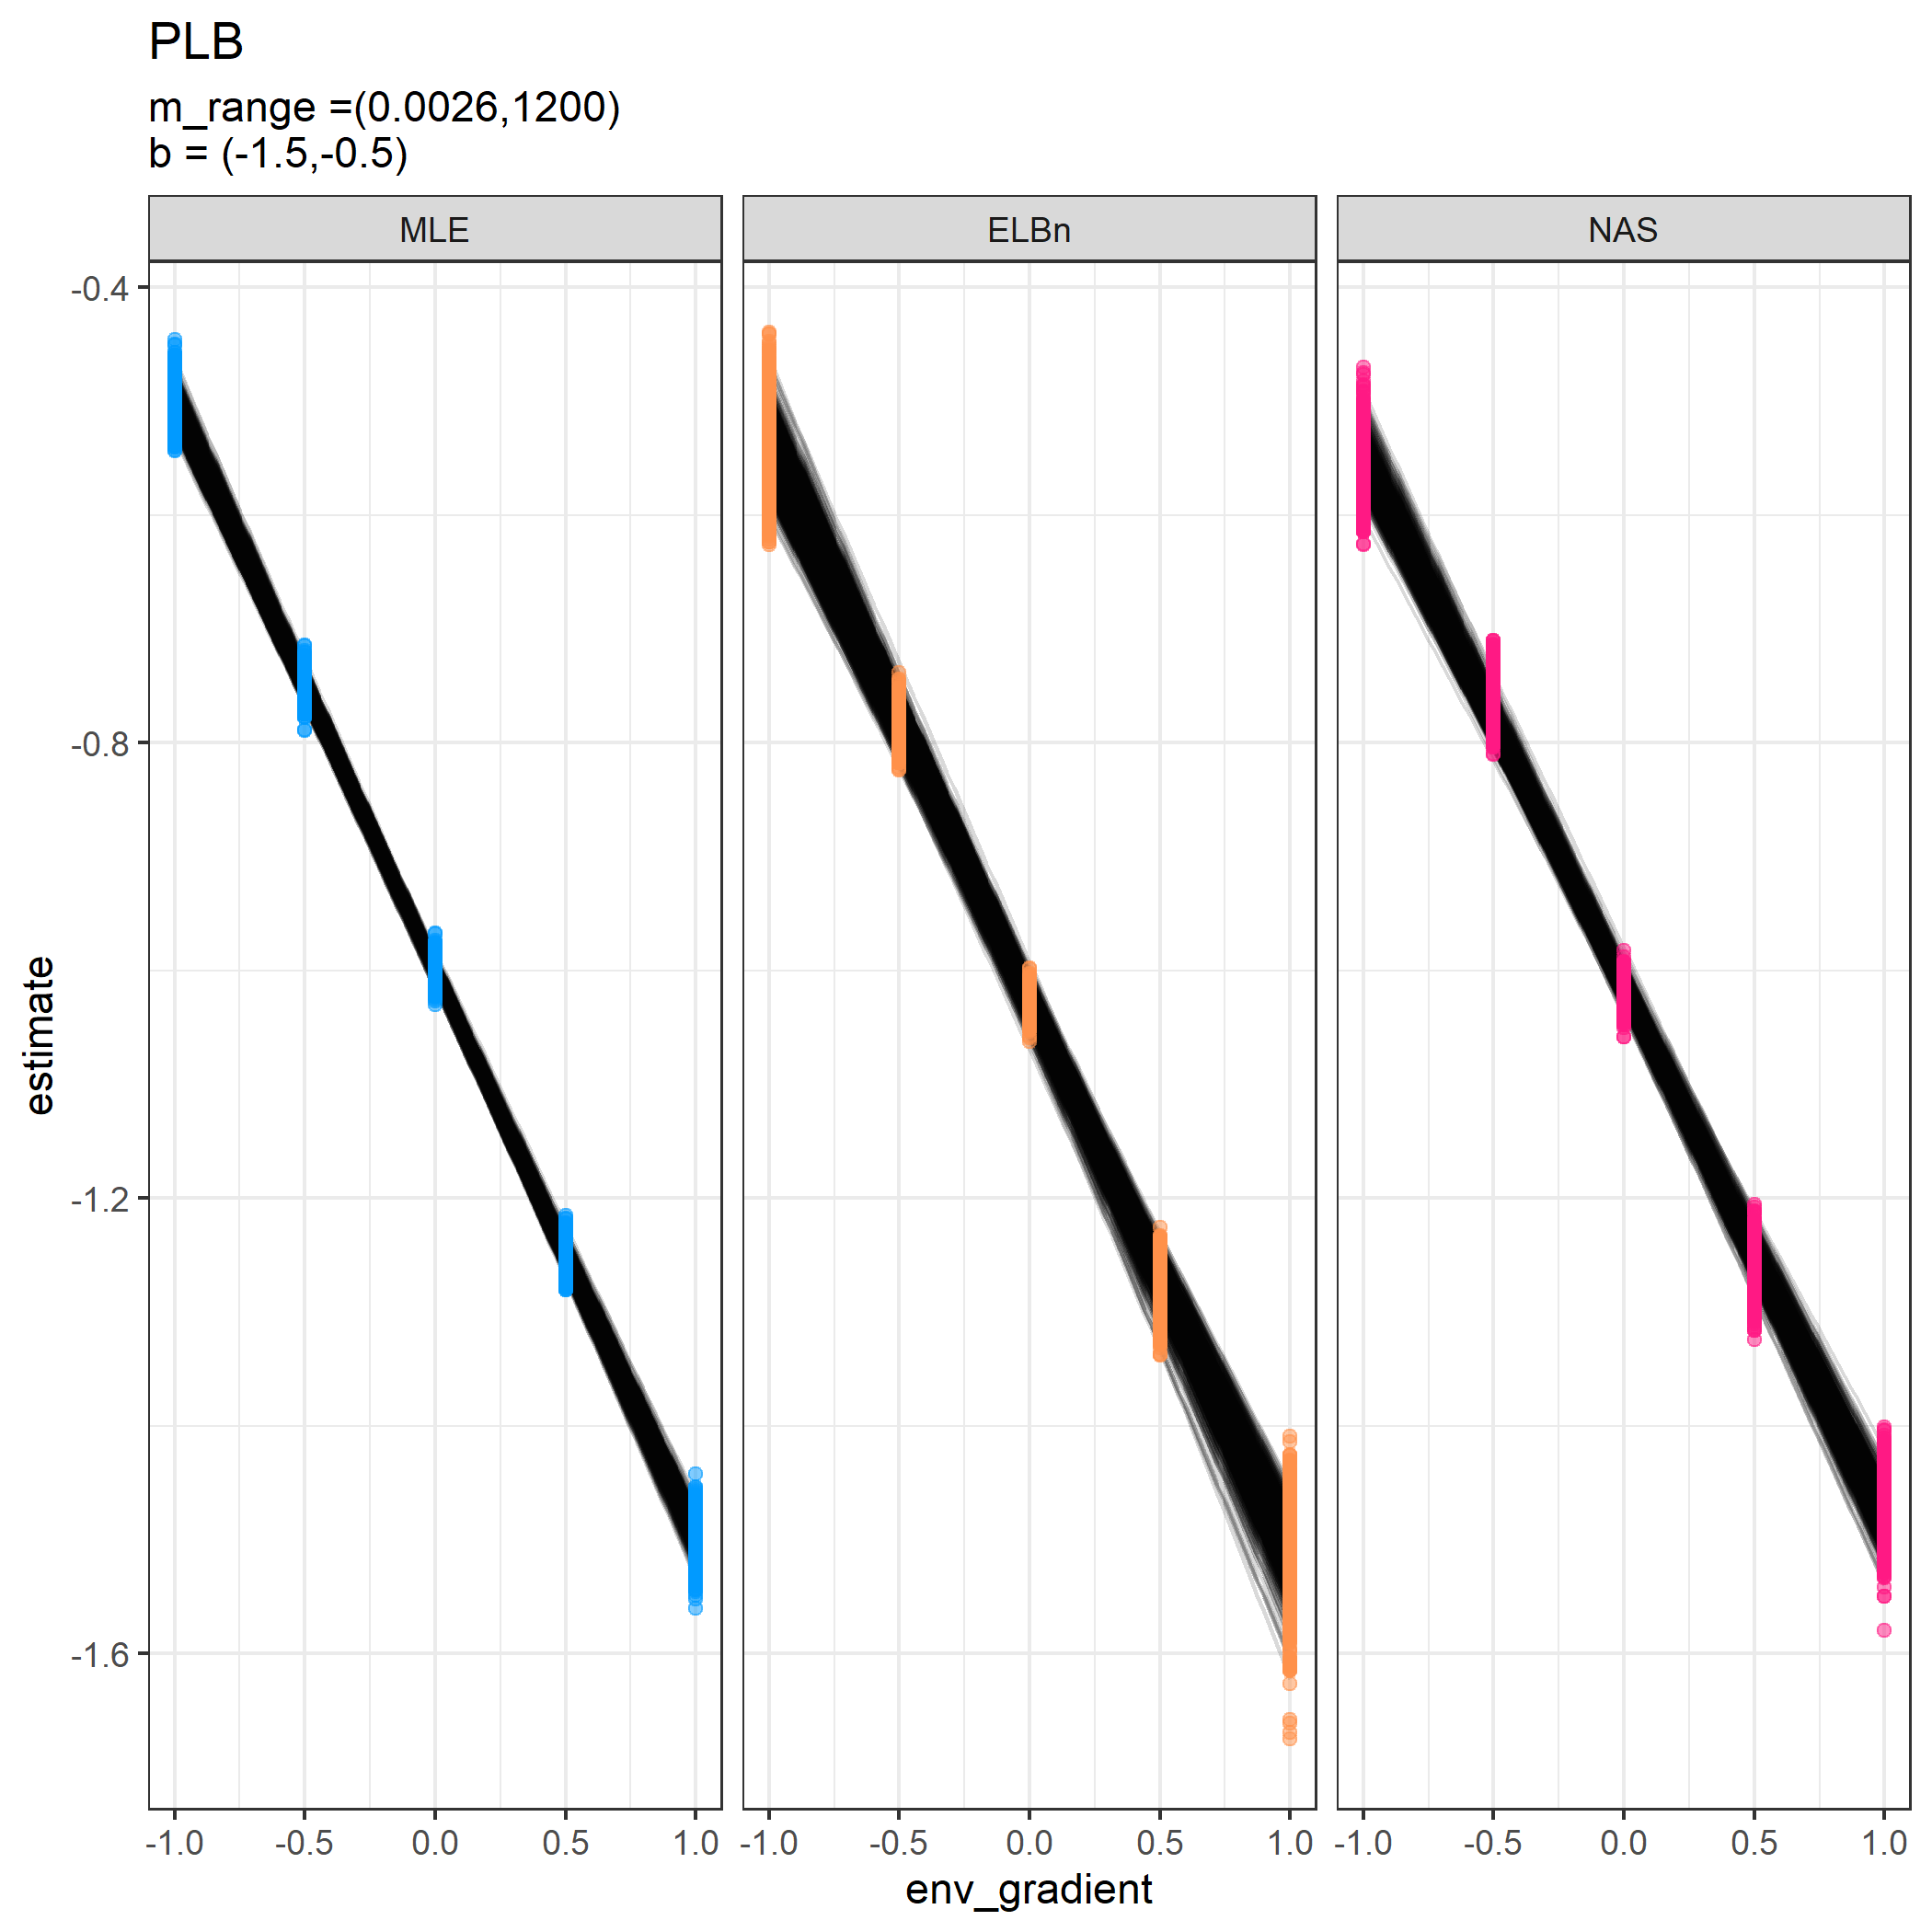
\includegraphics{figures/shallow_lambda_main.png}
\caption{Relationship estimates across the hypothetical gradient for
each replicate. Each panel is a different method for estimating the size
spectra parameter.}
\end{figure}

We found generally less variability in the relationship estimates across
a gradient of distributions described with shallower \(\lambda\)
parameters. All of the relationship coefficient estimates
(\(\beta_1\))'s across all replicates were significant regardless of
method used. The confidence interval for \(\beta_1\) estimate for the
MLE method contained the true value 94.7\% of the time. However, the
true value was in the confidence interval for the ELBN and NAS method
only 90.9\% and 76.9\% of the time, respectively. Once again, the mean
width of the CI for the binning methods were \textasciitilde2 times as
large as for the MLE method. Mean \(\pm\) SD CI width: MLE = 0.0442
\(\pm\) 0.0196; ELBn = 0.0920 \(\pm\) 0.0482, NAS = 0.0798 \(\pm\)
0.0324.

On average, the relationship across the gradient was under estimated,
but by nearly an order of magnitude less than when simulating across
steeper values of \(\lambda\). Differences between known and estimated
relationship coefficients: MLE -0.0007 (\(\pm\) 0.0079); ELBn -0.0058
(\(\pm\) 0.0177); NAS -0.0251 (\(\pm\) 0.0124).

\begin{figure}
\centering
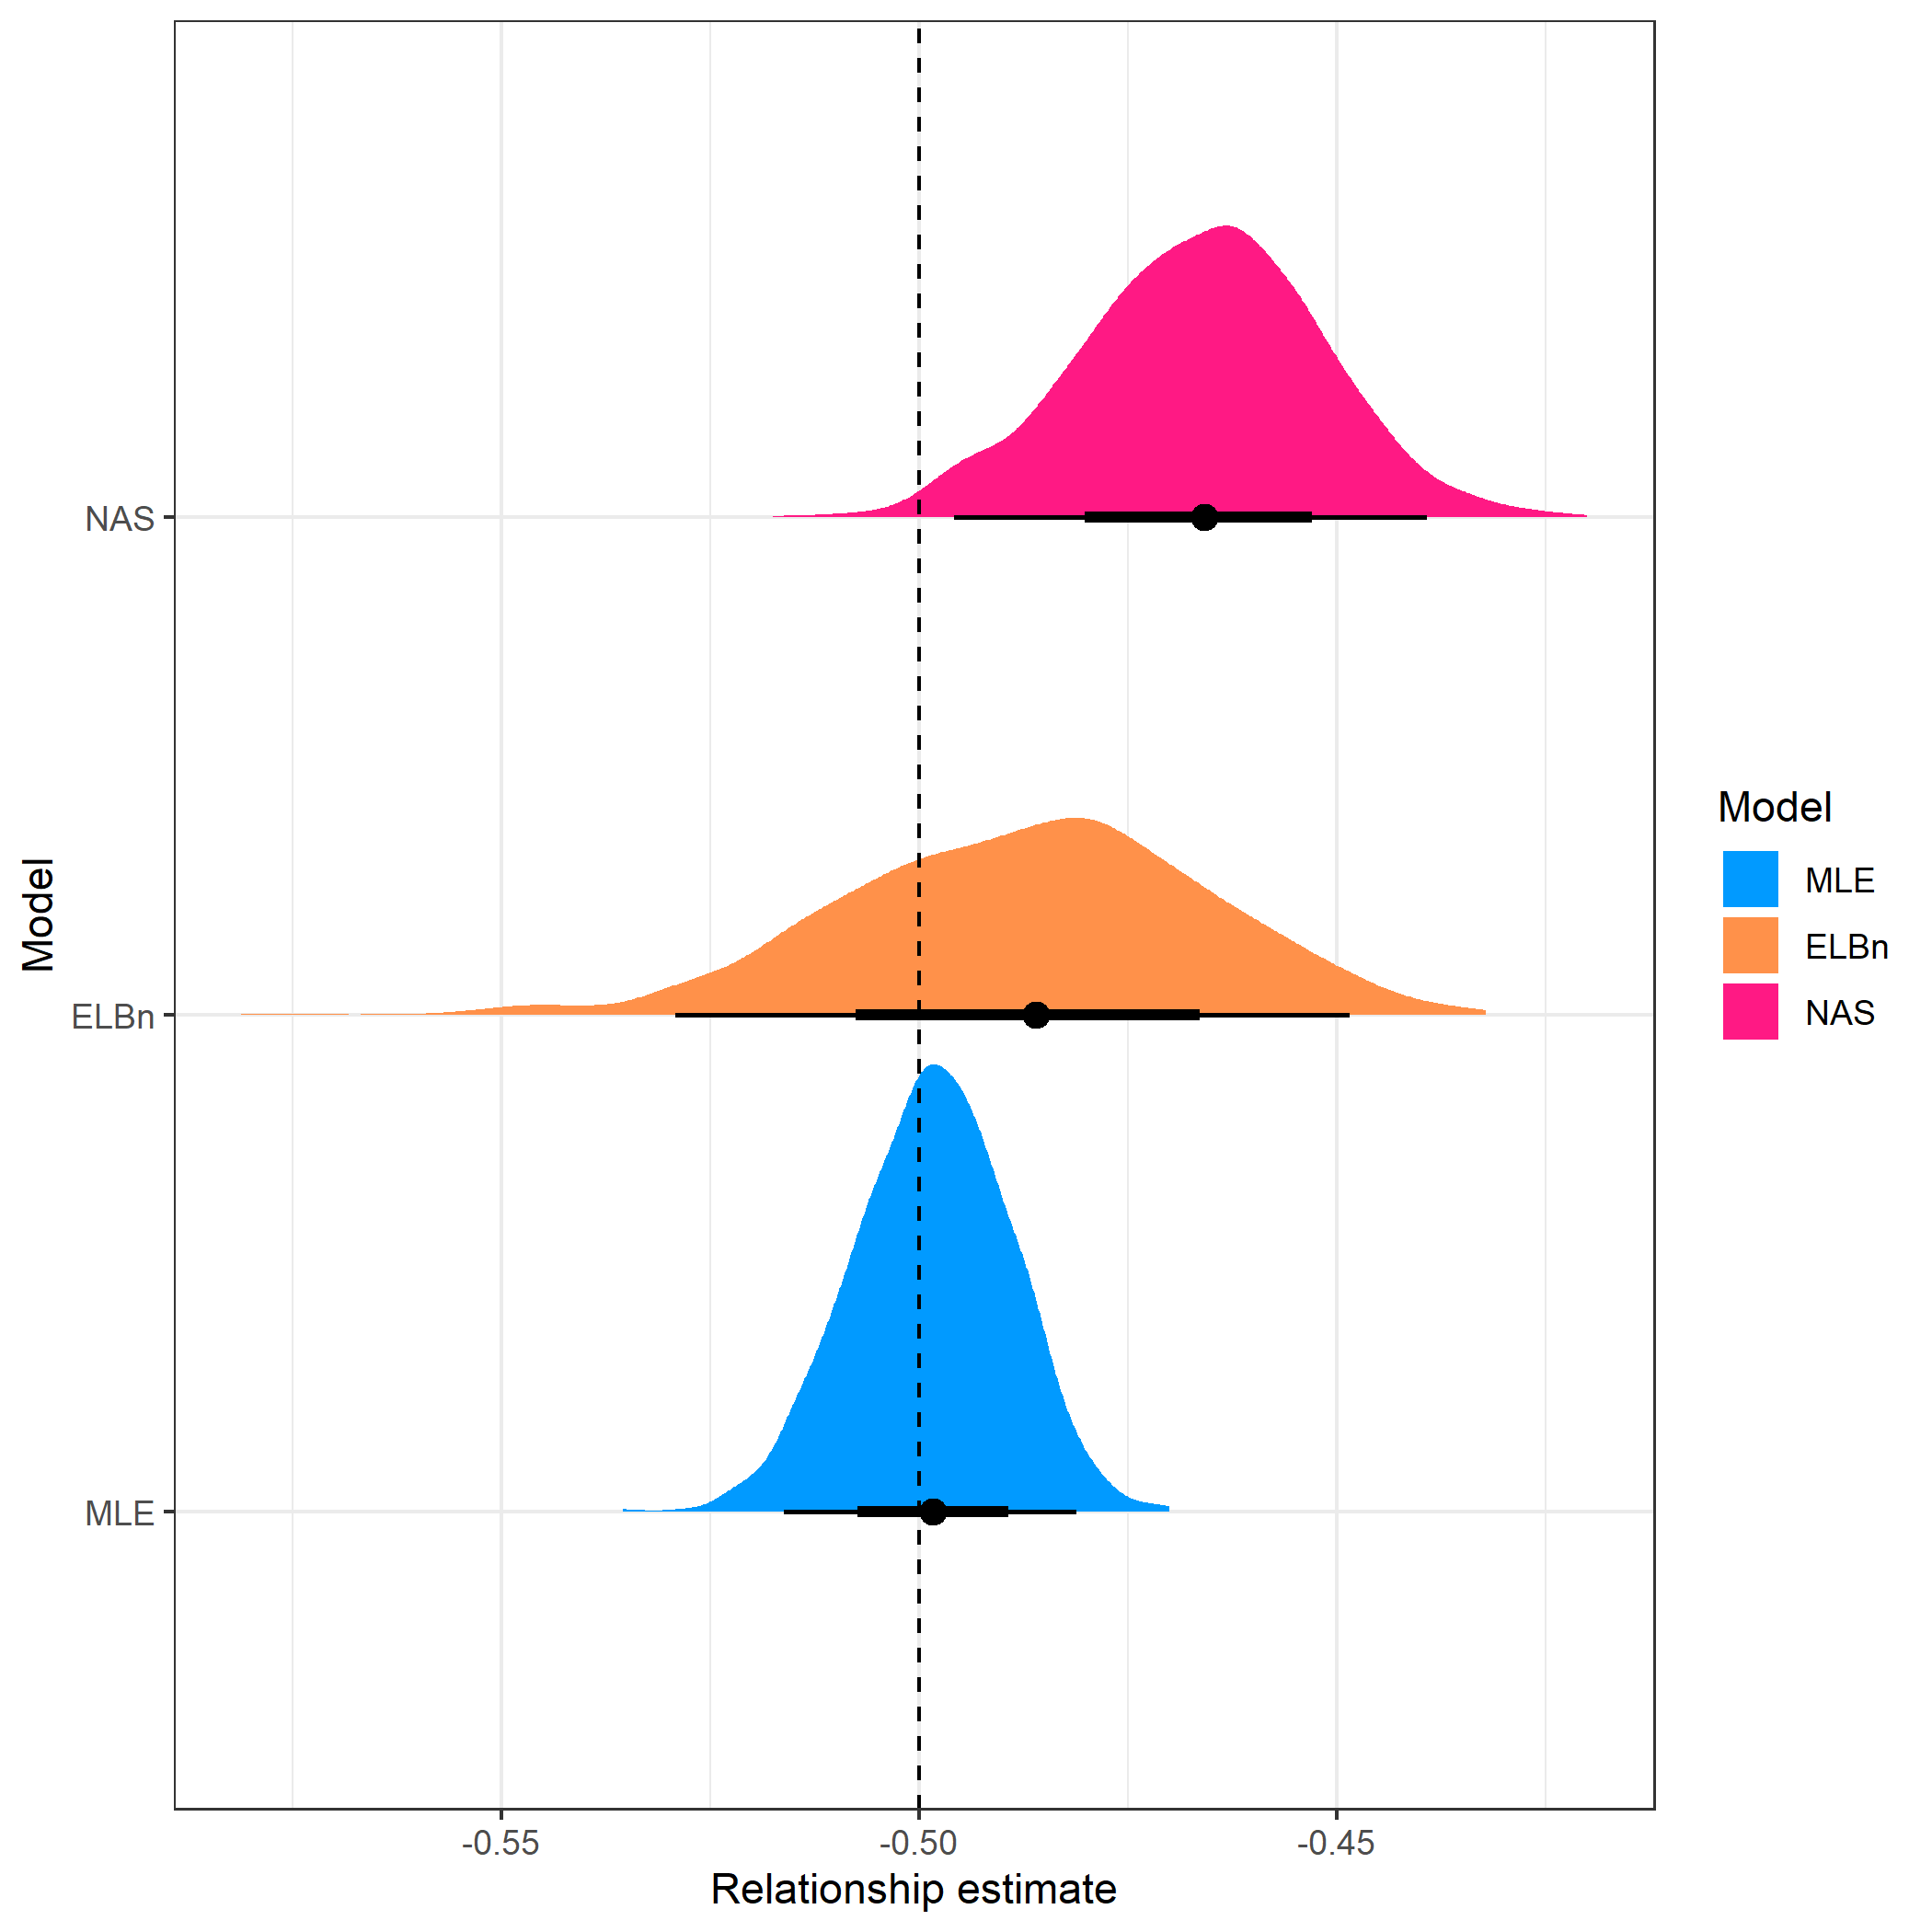
\includegraphics{figures/shallow_lambda_relationship_density.png}
\caption{Distribution of relationship coefficient estimates. Vertical
line is the known relationship. All methods under estimate the value,
but the mean magnitude and distribution of values is greater for the
ELBn and NAS methods.}
\end{figure}

\hypertarget{discussion}{%
\section{Discussion}\label{discussion}}

Measuring parameters describing the decline in abundance with increasing
body size in communities is being done with increasing frequency across
ecology. Previous work has investigated the accuracy and inherent biases
associated with different estimation methods. However, how these
innaccuracies and biases compound across environmental gradients remains
uncertain, making it difficult to detecting variation in size spectra
parameters across environmental gradients with confidence. Here, we
sampled body sizes from known distributions and estimated their
parameters across a hypothetical gradient in order to assess the
relationship coefficients obtained.

Generally, there was large agreement in the direction and magnitude of
average relationship coefficient estimates across methods. The estimate
from the MLE method was always closer to the known relationship, and
always had the smallest variation around the estimate.

All of the methods performed equally well when the \(\lambda\) value did
not vary across the hypothetical gradient, with a Type I error rate of
\textasciitilde5\%, exactly as would be expected under the assumptions
of frequentist statistics. This indicates that previous studies which
have detected no difference in size spectra parameters across sites can
be interpreted with confidence, regardless of the method used.

The performance of all methods improved as sample size increases, and as
the exponent of the size spectra relationship gets larger (more
shallow). As either or both of these variables change, the difference in
estimated relationship coefficients declines across the methods. This is
particularly interesting given the fact that both empirical data sets of
stream communities examined here are shallower than the expected
relationship of \(\lambda = -2\), and the conclusions of the change in
size spectra relationships across the gradients are not dependent on
method used. If communities under study are in fact described by
shallower exponents, the method used may not be critical in the
conclusions reached. However, the MLE method performs as well or better
than the two binning methods examined here under all contexts and should
be the preferred method moving forward. At a minimum, future studies
should report MLE estimates to ensure that the results are not dependent
on the methodology used.

Alarmingly, the performance of all methods declined dramatically when
trying to detect smaller variation in \(\lambda\) values. We simulated
observations from distributions varying by an absolute value of 0.2
units. This range of variation is similar to that which has been
reported in many seminal works on variation in size spectra parameters.
When using the MLE method, significant relationships were only detected
\textasciitilde88\% of the time, whereas both of the binning methods
only detected significant trends \textasciitilde20\% of the time. Of the
simulation replicates which were significant, nearly all of them were
negative across all methods except for one single replicate using the
NAS method which was positive (Figure. 5).

Despite the drop in performance with reduced variation in \(\lambda\)
values, when a significant relationship was observed, it was generally
in the correct direction and of a similar magnitude. This suggests that
previously reported significant changes in size spectra parameters
across environmental gradients and in experimental manipulations are
plausible, and the magnitude of the relative change is a reasonable
estimate. Given that all of the data within a study is treated
identically, the the over all chnage in size spectra parameters is
likely reasonable. However, the biases and inconsistencies in
relationship estimates presented here suggest that it would be difficult
if not impossible to compare the relative changes across different
published studies which use different methods. Publication of individual
body size data with future studies of size spectra relationships would
greatly aid in our ability to generalize changes to this fundamental
aspect of community organization across spatiotemporal scales and in
response to environmental stressors and perturbations.

\hypertarget{concluding-remarks}{%
\subsection{Concluding Remarks}\label{concluding-remarks}}

We reiterate the recommendations of White et al.~(2007)(2007), Sprules
and Barth (2016)(2016) and Edwards et al.~(2017)(2017) to estimate size
spectra relationships using MLE methods due to their superior
performance in nearly every context. Furthermore, we strongly encourage
authors to publish individual size data whenever possible. This will
allow for the consistent re-analysis of existing data sets as
methodologies develop and improve. This will aid in the ability for size
spectra work to be synthesized between research groups and across
scales.

\hypertarget{references}{%
\section{References}\label{references}}

\hypertarget{refs}{}
\begin{CSLReferences}{1}{0}
\leavevmode\vadjust pre{\hypertarget{ref-dossena2012}{}}%
Dossena, M., G. Yvon-Durocher, J. Grey, J. M. Montoya, D. M. Perkins, M.
Trimmer, and G. Woodward. 2012.
\href{https://doi.org/10.1098/rspb.2012.0394}{Warming alters community
size structure and ecosystem functioning}. Proceedings of the Royal
Society B: Biological Sciences 279:3011--3019.

\leavevmode\vadjust pre{\hypertarget{ref-edwards2020}{}}%
Edwards, A. M., J. P. W. Robinson, J. L. Blanchard, J. K. Baum, and M.
J. Plank. 2020. \href{https://doi.org/10.3354/meps13230}{Accounting for
the bin structure of data removes bias when fitting size spectra}.
Marine Ecology Progress Series 636:19--33.

\leavevmode\vadjust pre{\hypertarget{ref-edwards2017}{}}%
Edwards, A. M., J. P. W. Robinson, M. J. Plank, J. K. Baum, and J. L.
Blanchard. 2017. \href{https://doi.org/10.1111/2041-210X.12641}{Testing
and recommending methods for fitting size spectra to data}. Methods in
Ecology and Evolution 8:57--67.

\leavevmode\vadjust pre{\hypertarget{ref-mcgarvey2018}{}}%
McGarvey, D. J., and A. J. Kirk. 2018.
\href{https://doi.org/10.1007/s10750-017-3448-0}{Seasonal comparison of
community-level size-spectra in southern coalfield streams of {West
Virginia} ({USA})}. Hydrobiologia 809:65--77.

\leavevmode\vadjust pre{\hypertarget{ref-mcgarvey2019}{}}%
McGarvey, D. J., T. E. Woods, and A. J. Kirk. 2019.
\href{https://doi.org/10.3791/59945}{Modeling the {Size Spectrum} for
{Macroinvertebrates} and {Fishes} in {Stream Ecosystems}}. Journal of
Visualized Experiments: JoVE.

\leavevmode\vadjust pre{\hypertarget{ref-NEON_Inverts2022}{}}%
National Ecological Observatory Network (NEON). 2022.
\href{https://doi.org/10.48443/GN8X-K322}{Macroinvertebrate collection
({DP1}.20120.001)}. {National Ecological Observatory Network (NEON)}.

\leavevmode\vadjust pre{\hypertarget{ref-ogorman2017}{}}%
O'Gorman, E. J., L. Zhao, D. E. Pichler, G. Adams, N. Friberg, B. C.
Rall, A. Seeney, H. Zhang, D. C. Reuman, and G. Woodward. 2017.
\href{https://doi.org/10.1038/nclimate3368}{Unexpected changes in
community size structure in a natural warming experiment}. Nature
Climate Change 7:659--663.

\leavevmode\vadjust pre{\hypertarget{ref-petchey2010}{}}%
Petchey, O. L., and A. Belgrano. 2010.
\href{https://doi.org/10.1098/rsbl.2010.0240}{Body-size distributions
and size-spectra: Universal indicators of ecological status?} Biology
Letters 6:434--437.

\leavevmode\vadjust pre{\hypertarget{ref-pomeranz2022}{}}%
Pomeranz, J. P. F., J. R. Junker, and J. S. Wesner. 2022.
\href{https://doi.org/10.1111/gcb.15862}{Individual size distributions
across {North American} streams vary with local temperature}. Global
Change Biology 28:848--858.

\leavevmode\vadjust pre{\hypertarget{ref-sprules2016}{}}%
Sprules, W. G., and L. E. Barth. 2016.
\href{https://doi.org/10.1139/cjfas-2015-0115}{Surfing the biomass size
spectrum: Some remarks on history, theory, and application}. Canadian
Journal of Fisheries and Aquatic Sciences 73:477--495.

\leavevmode\vadjust pre{\hypertarget{ref-white2007}{}}%
White, E. P., S. K. M. Ernest, A. J. Kerkhoff, and B. J. Enquist. 2007.
\href{https://doi.org/10.1016/j.tree.2007.03.007}{Relationships between
body size and abundance in ecology}. Trends in Ecology \& Evolution
22:323--330.

\end{CSLReferences}

\newpage

\hypertarget{supplementary-material}{%
\section*{Supplementary material}\label{supplementary-material}}
\addcontentsline{toc}{section}{Supplementary material}

\setcounter{table}{0} \renewcommand{\thetable}{S\arabic{table}} \setcounter{figure}{0} \renewcommand{\thefigure}{S\arabic{figure}}

\hypertarget{range-of-body-sizes-m}{%
\subsection{\texorpdfstring{Range of body sizes,
\(M\)}{Range of body sizes, M}}\label{range-of-body-sizes-m}}

\begin{figure}
\centering
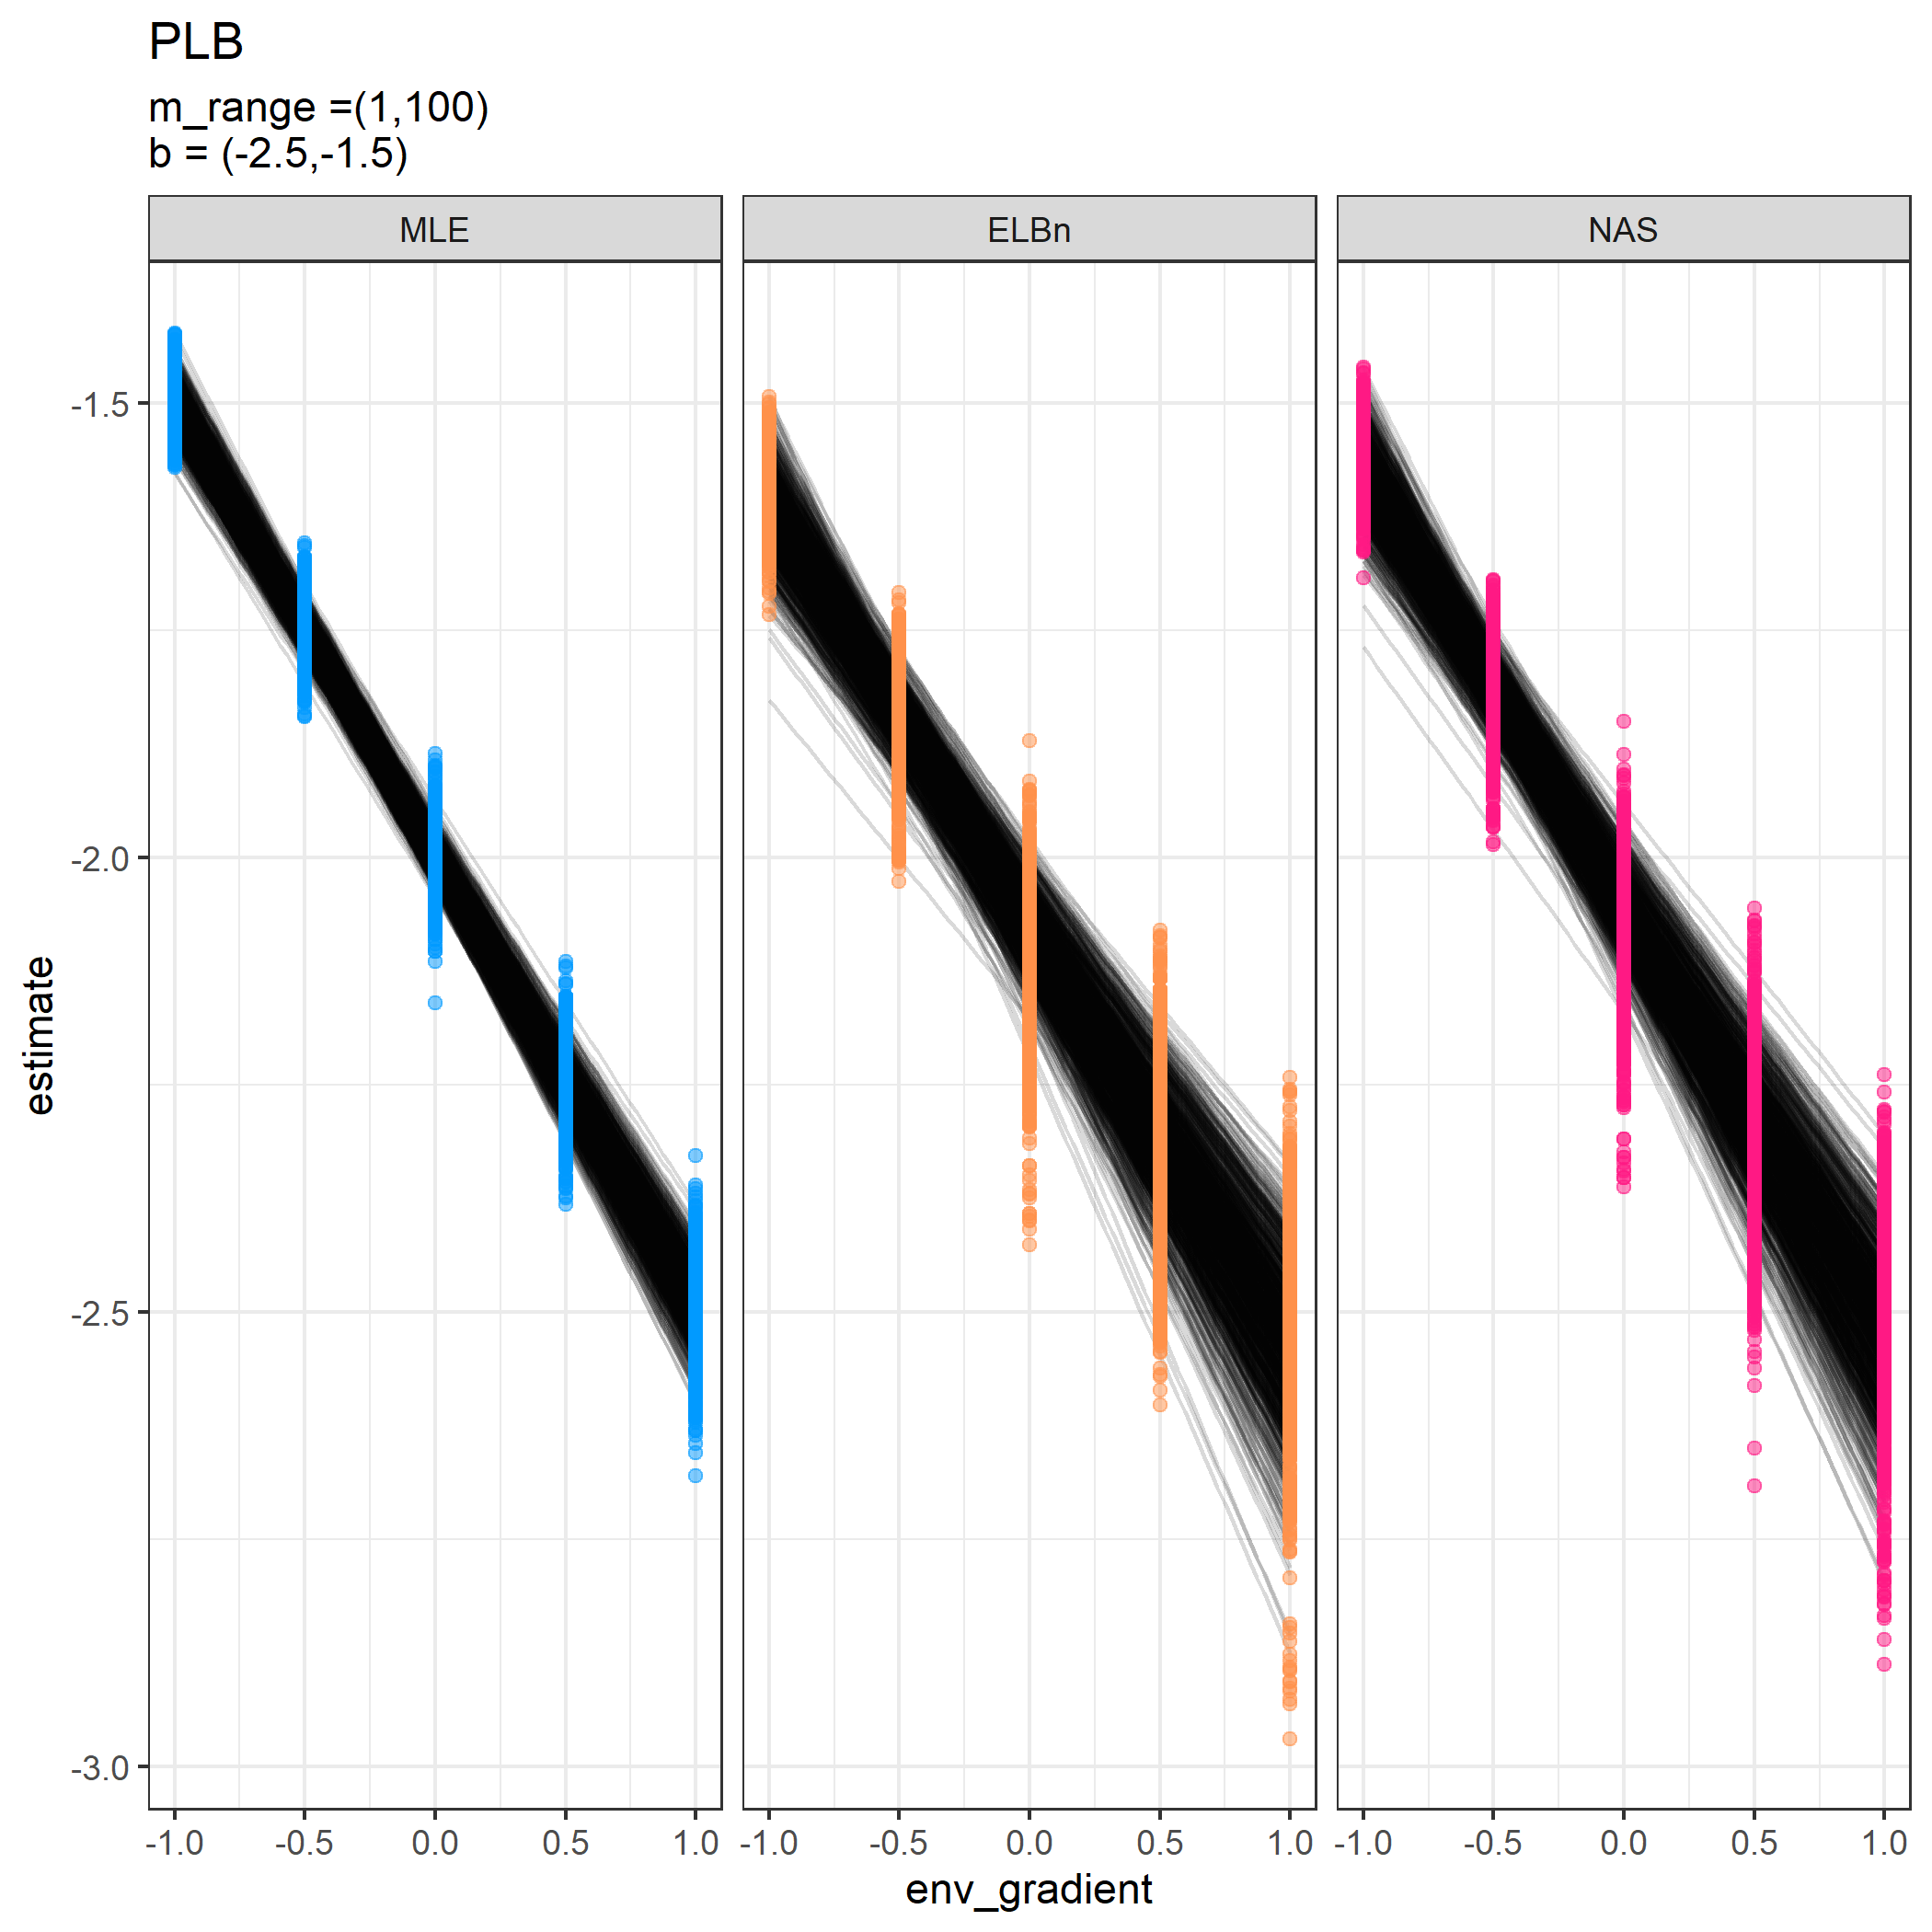
\includegraphics{figures/PLB_small_m_main.png}
\caption{Individual regressions for five sites across a hypothetical
gradient with a known relationship of 0.5. Range of body sizes is
reduced and is from 1, to 100.}
\end{figure}

\begin{figure}
\centering
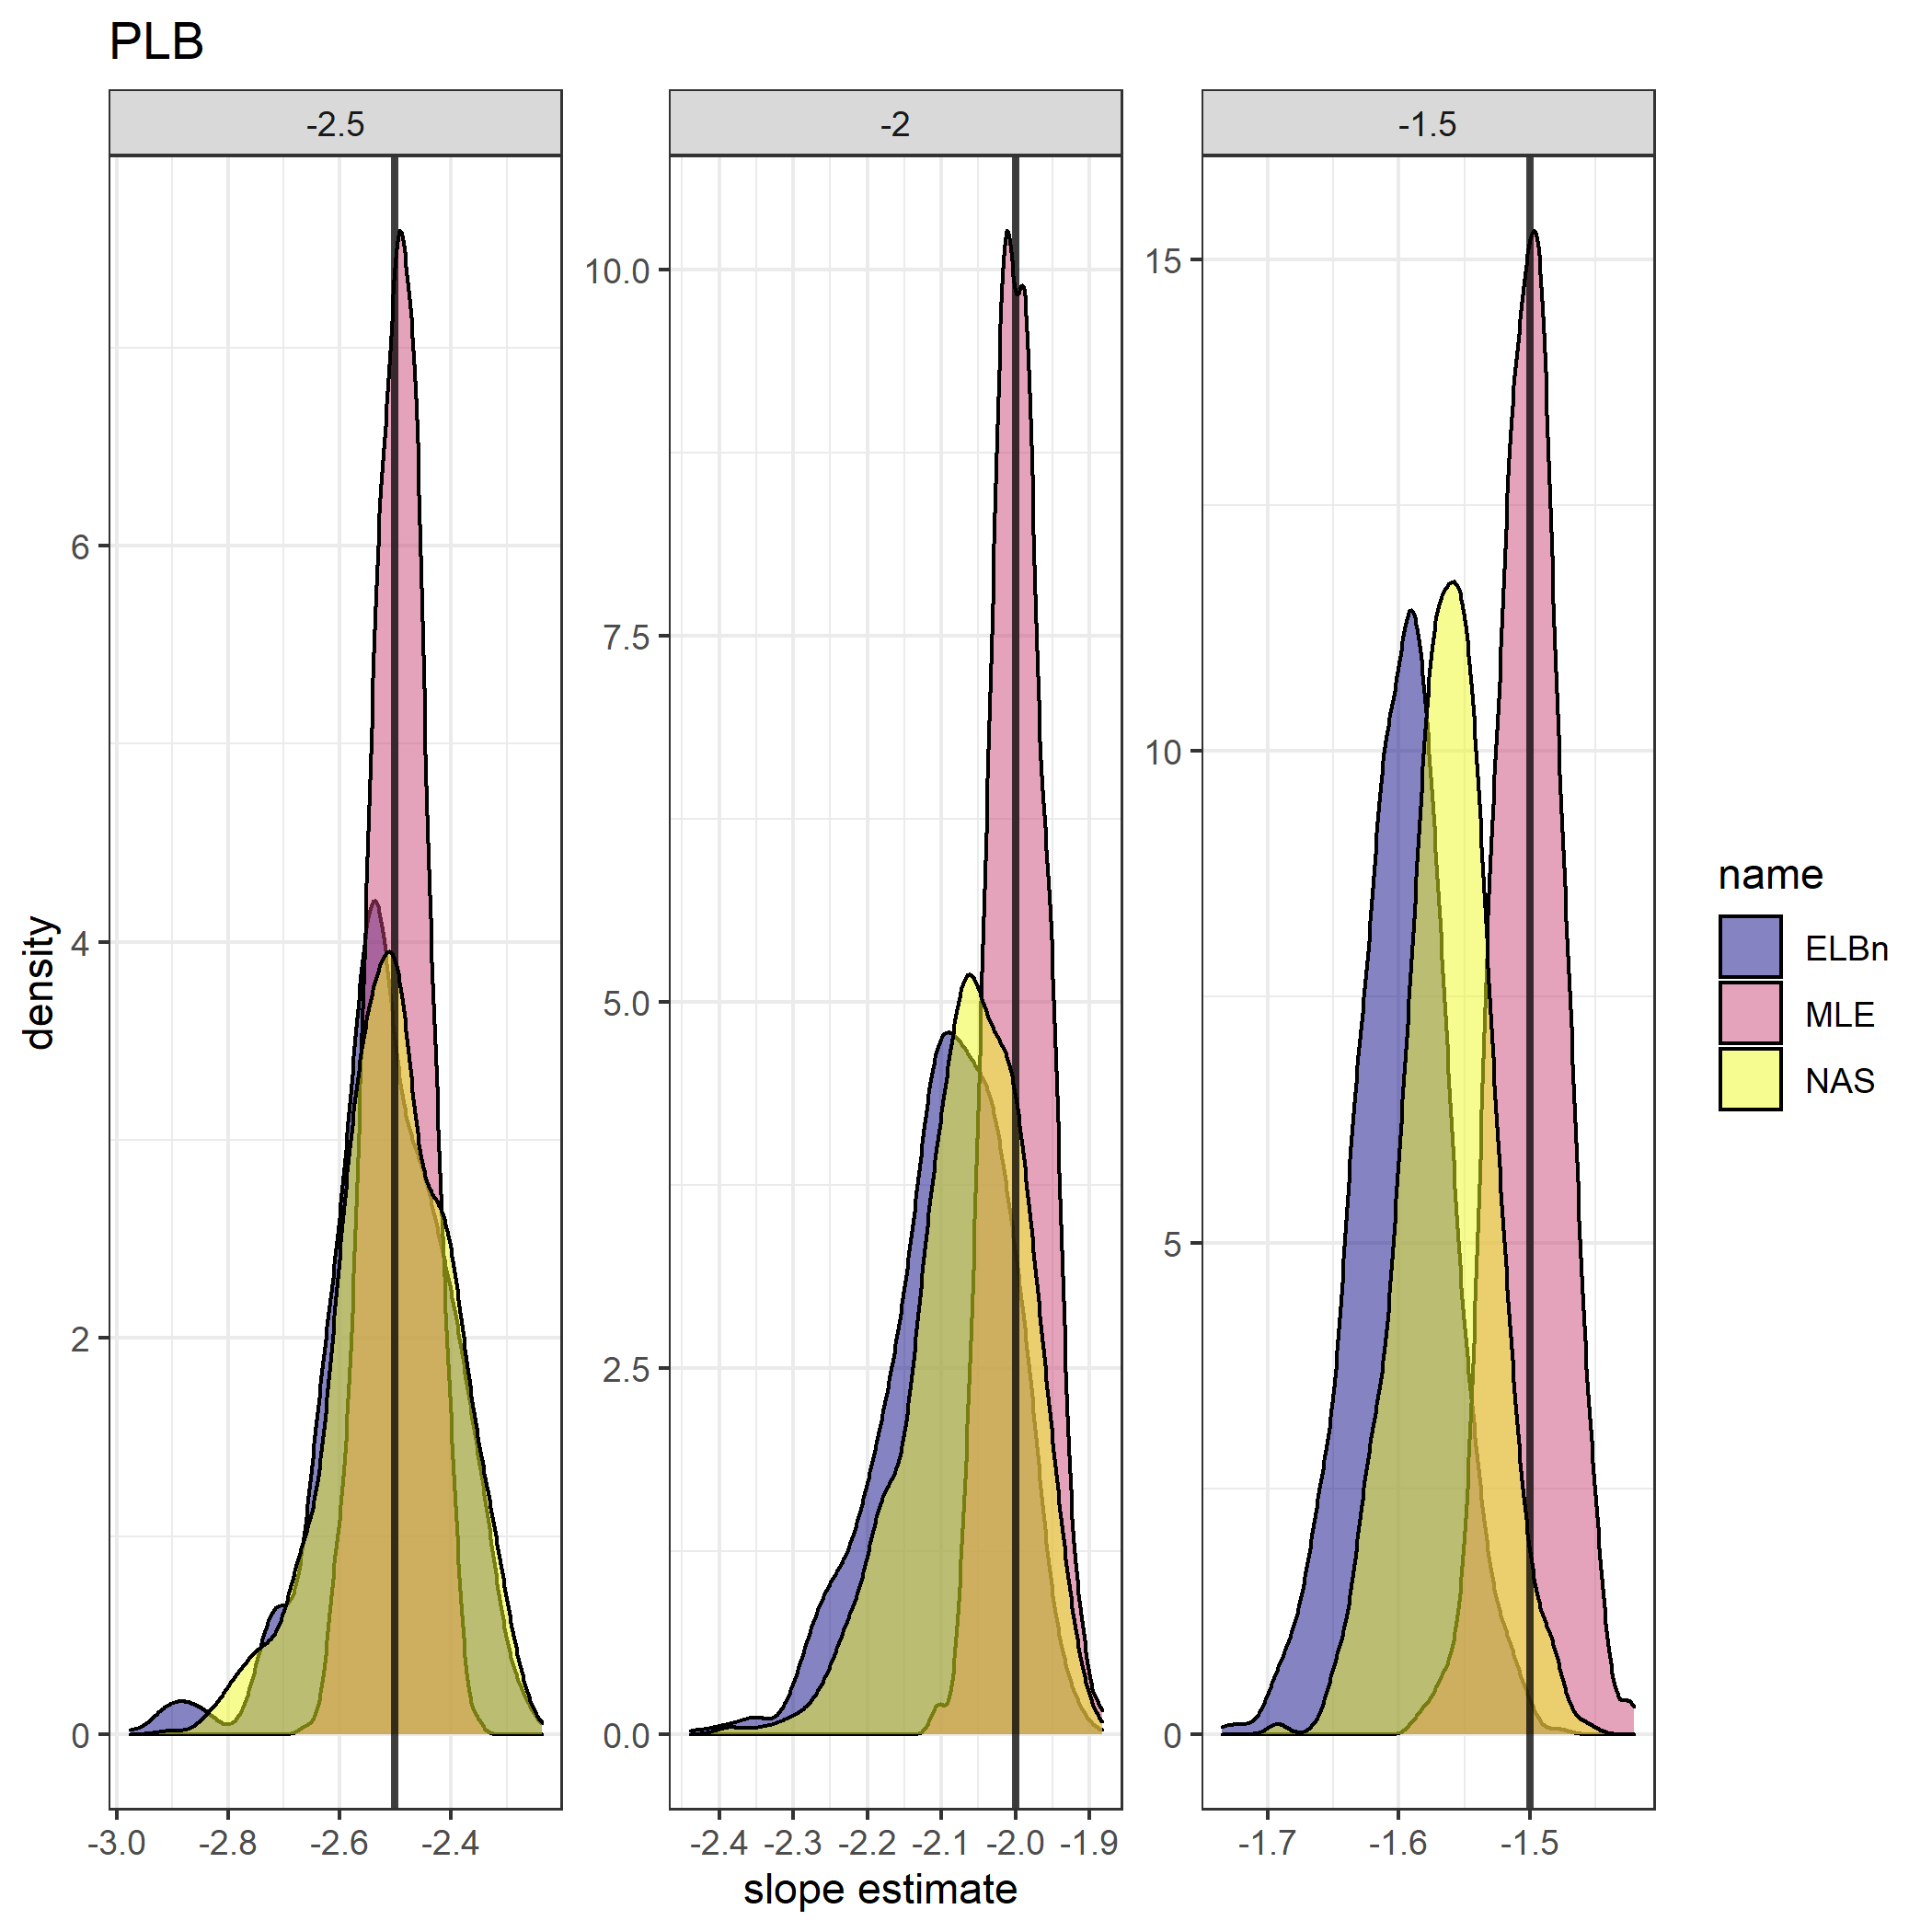
\includegraphics{figures/PLB_small_m_est_b_density.png}
\caption{Distribution of estimated \(\lambda\) coefficient for five
sites across a hypothetical gradient with known values. Range of body
sizes is reduced and is from 1, to 100.}
\end{figure}

\begin{figure}
\centering
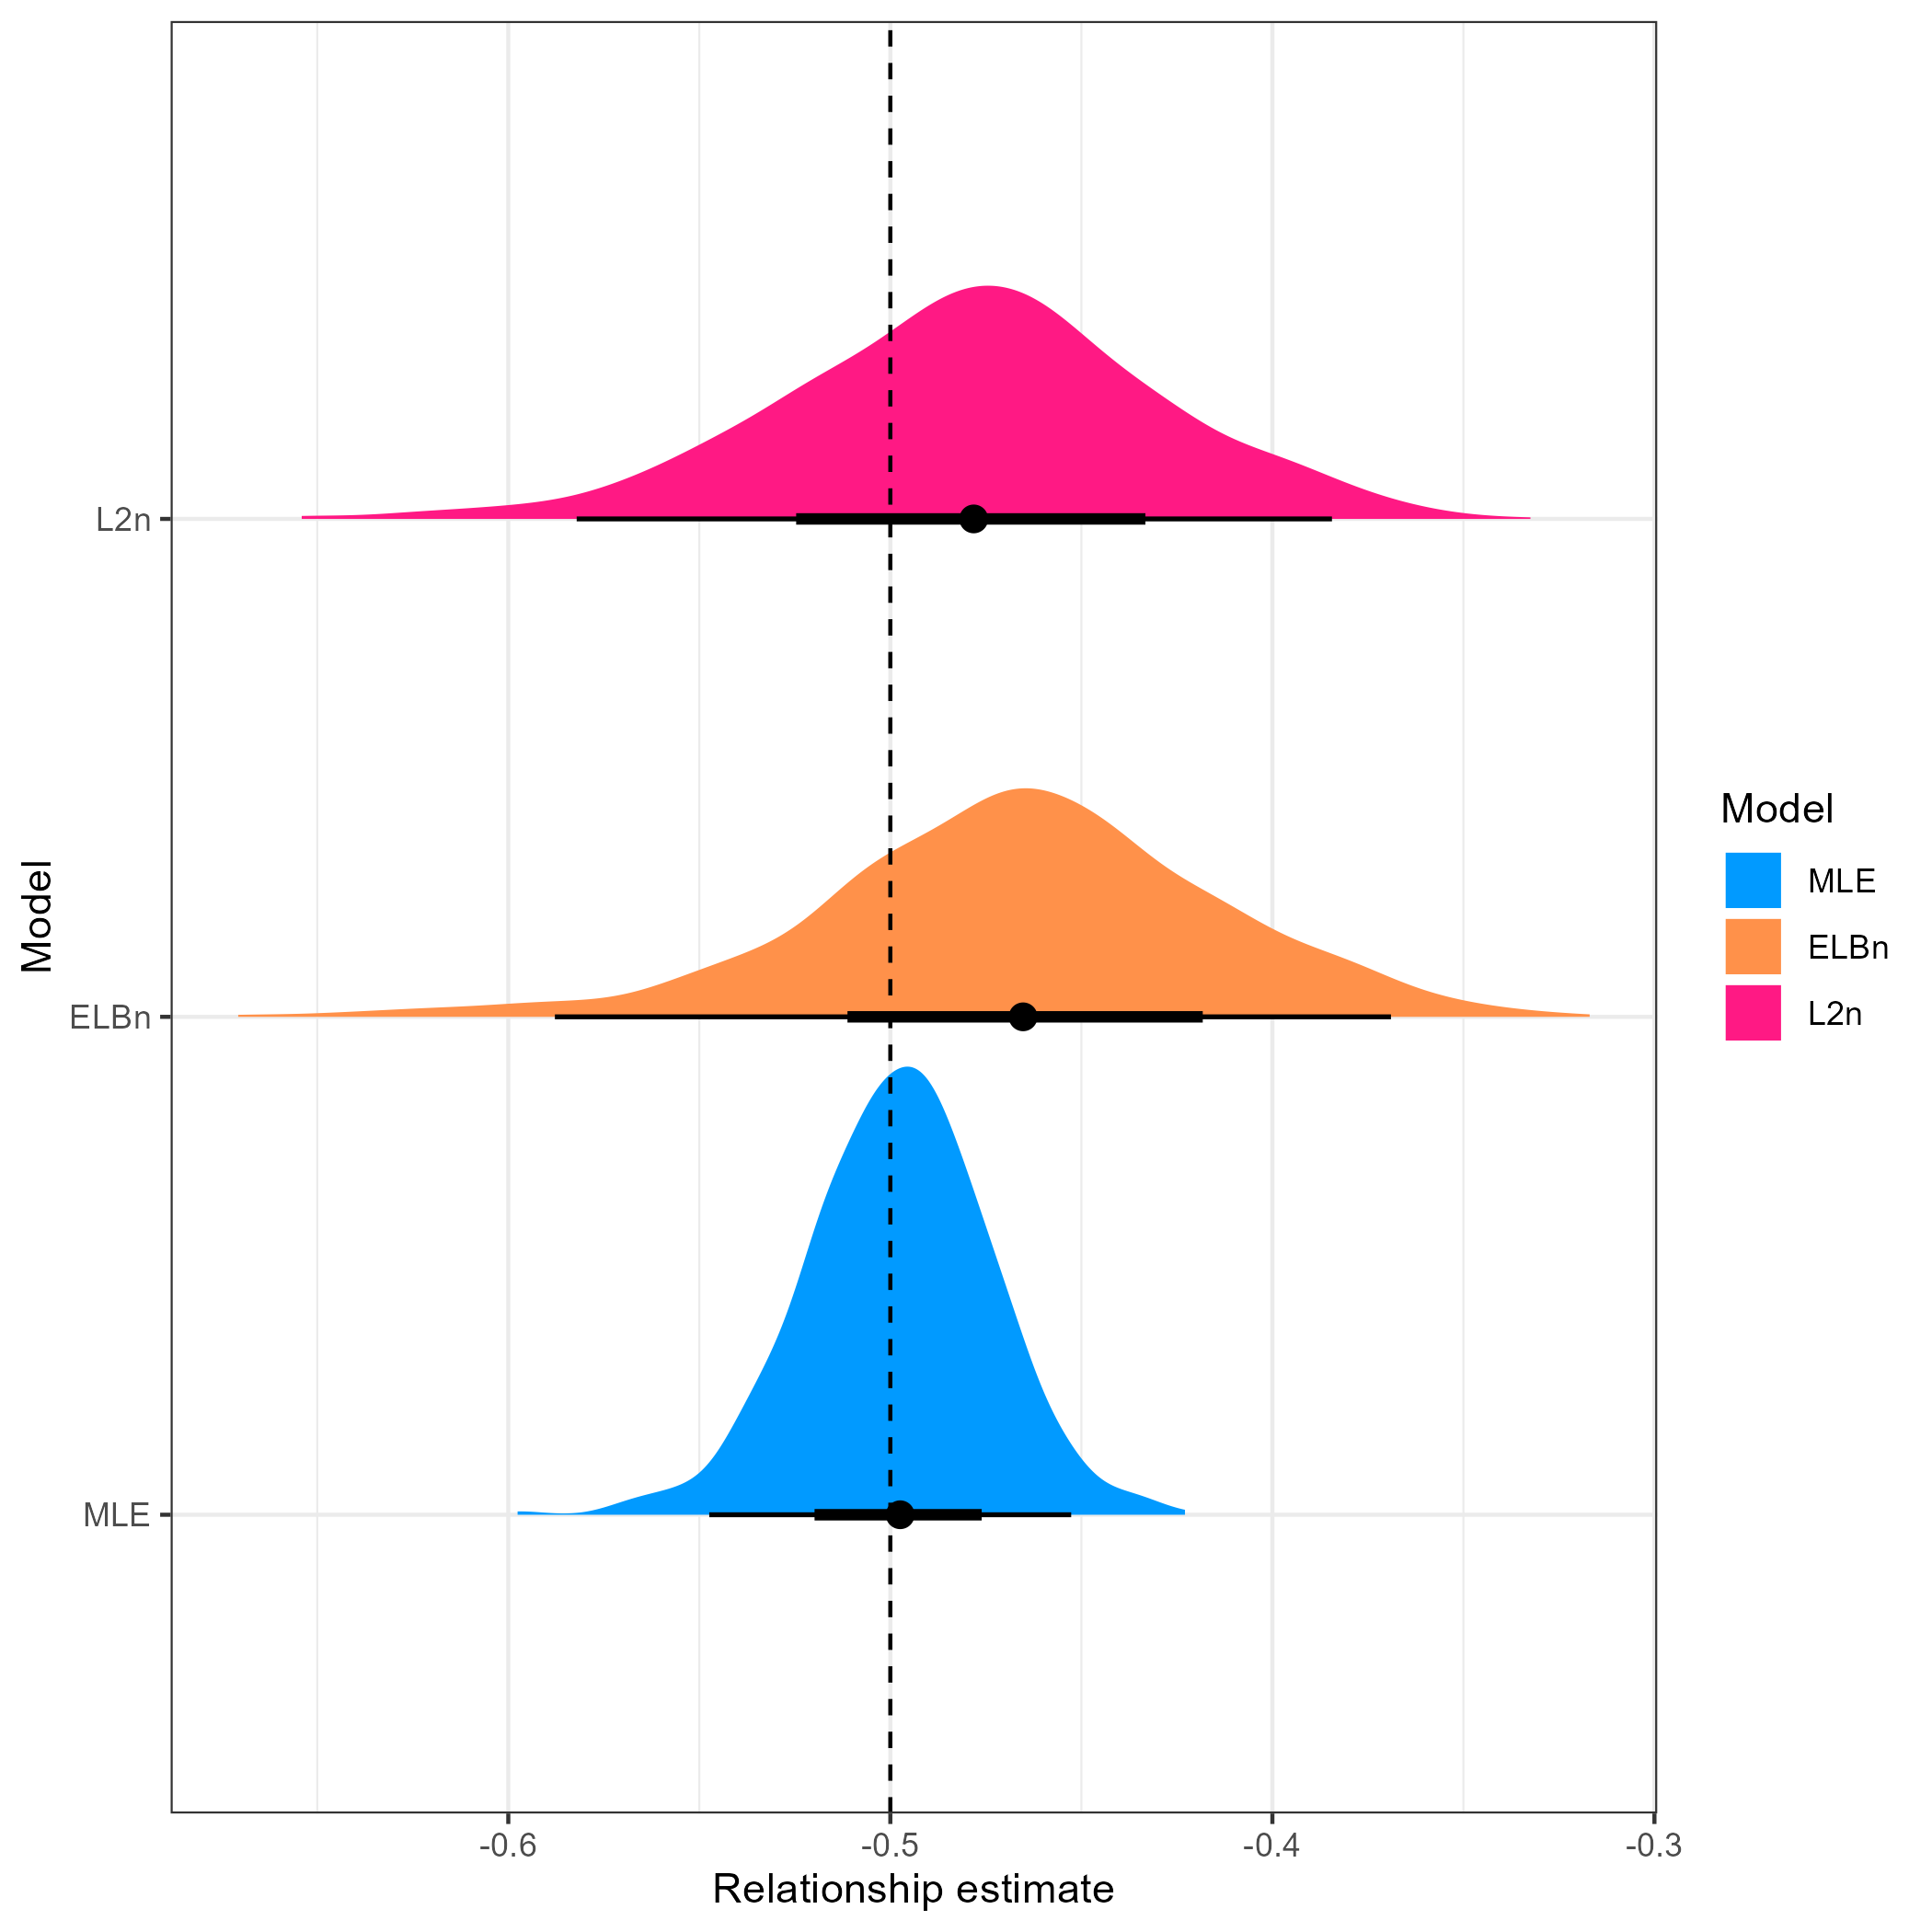
\includegraphics{figures/PLB_small_m_relationship_density.png}
\caption{Distribution of estimated relationship (\(\beta_1\))
coefficient's for five sites across a hypothetical gradient with known
value of 0.5. Range of body sizes is reduced and is from 1, to 100.}
\end{figure}

\hypertarget{large-environmental-gradient}{%
\subsection{Large environmental
gradient}\label{large-environmental-gradient}}

\begin{figure}
\centering
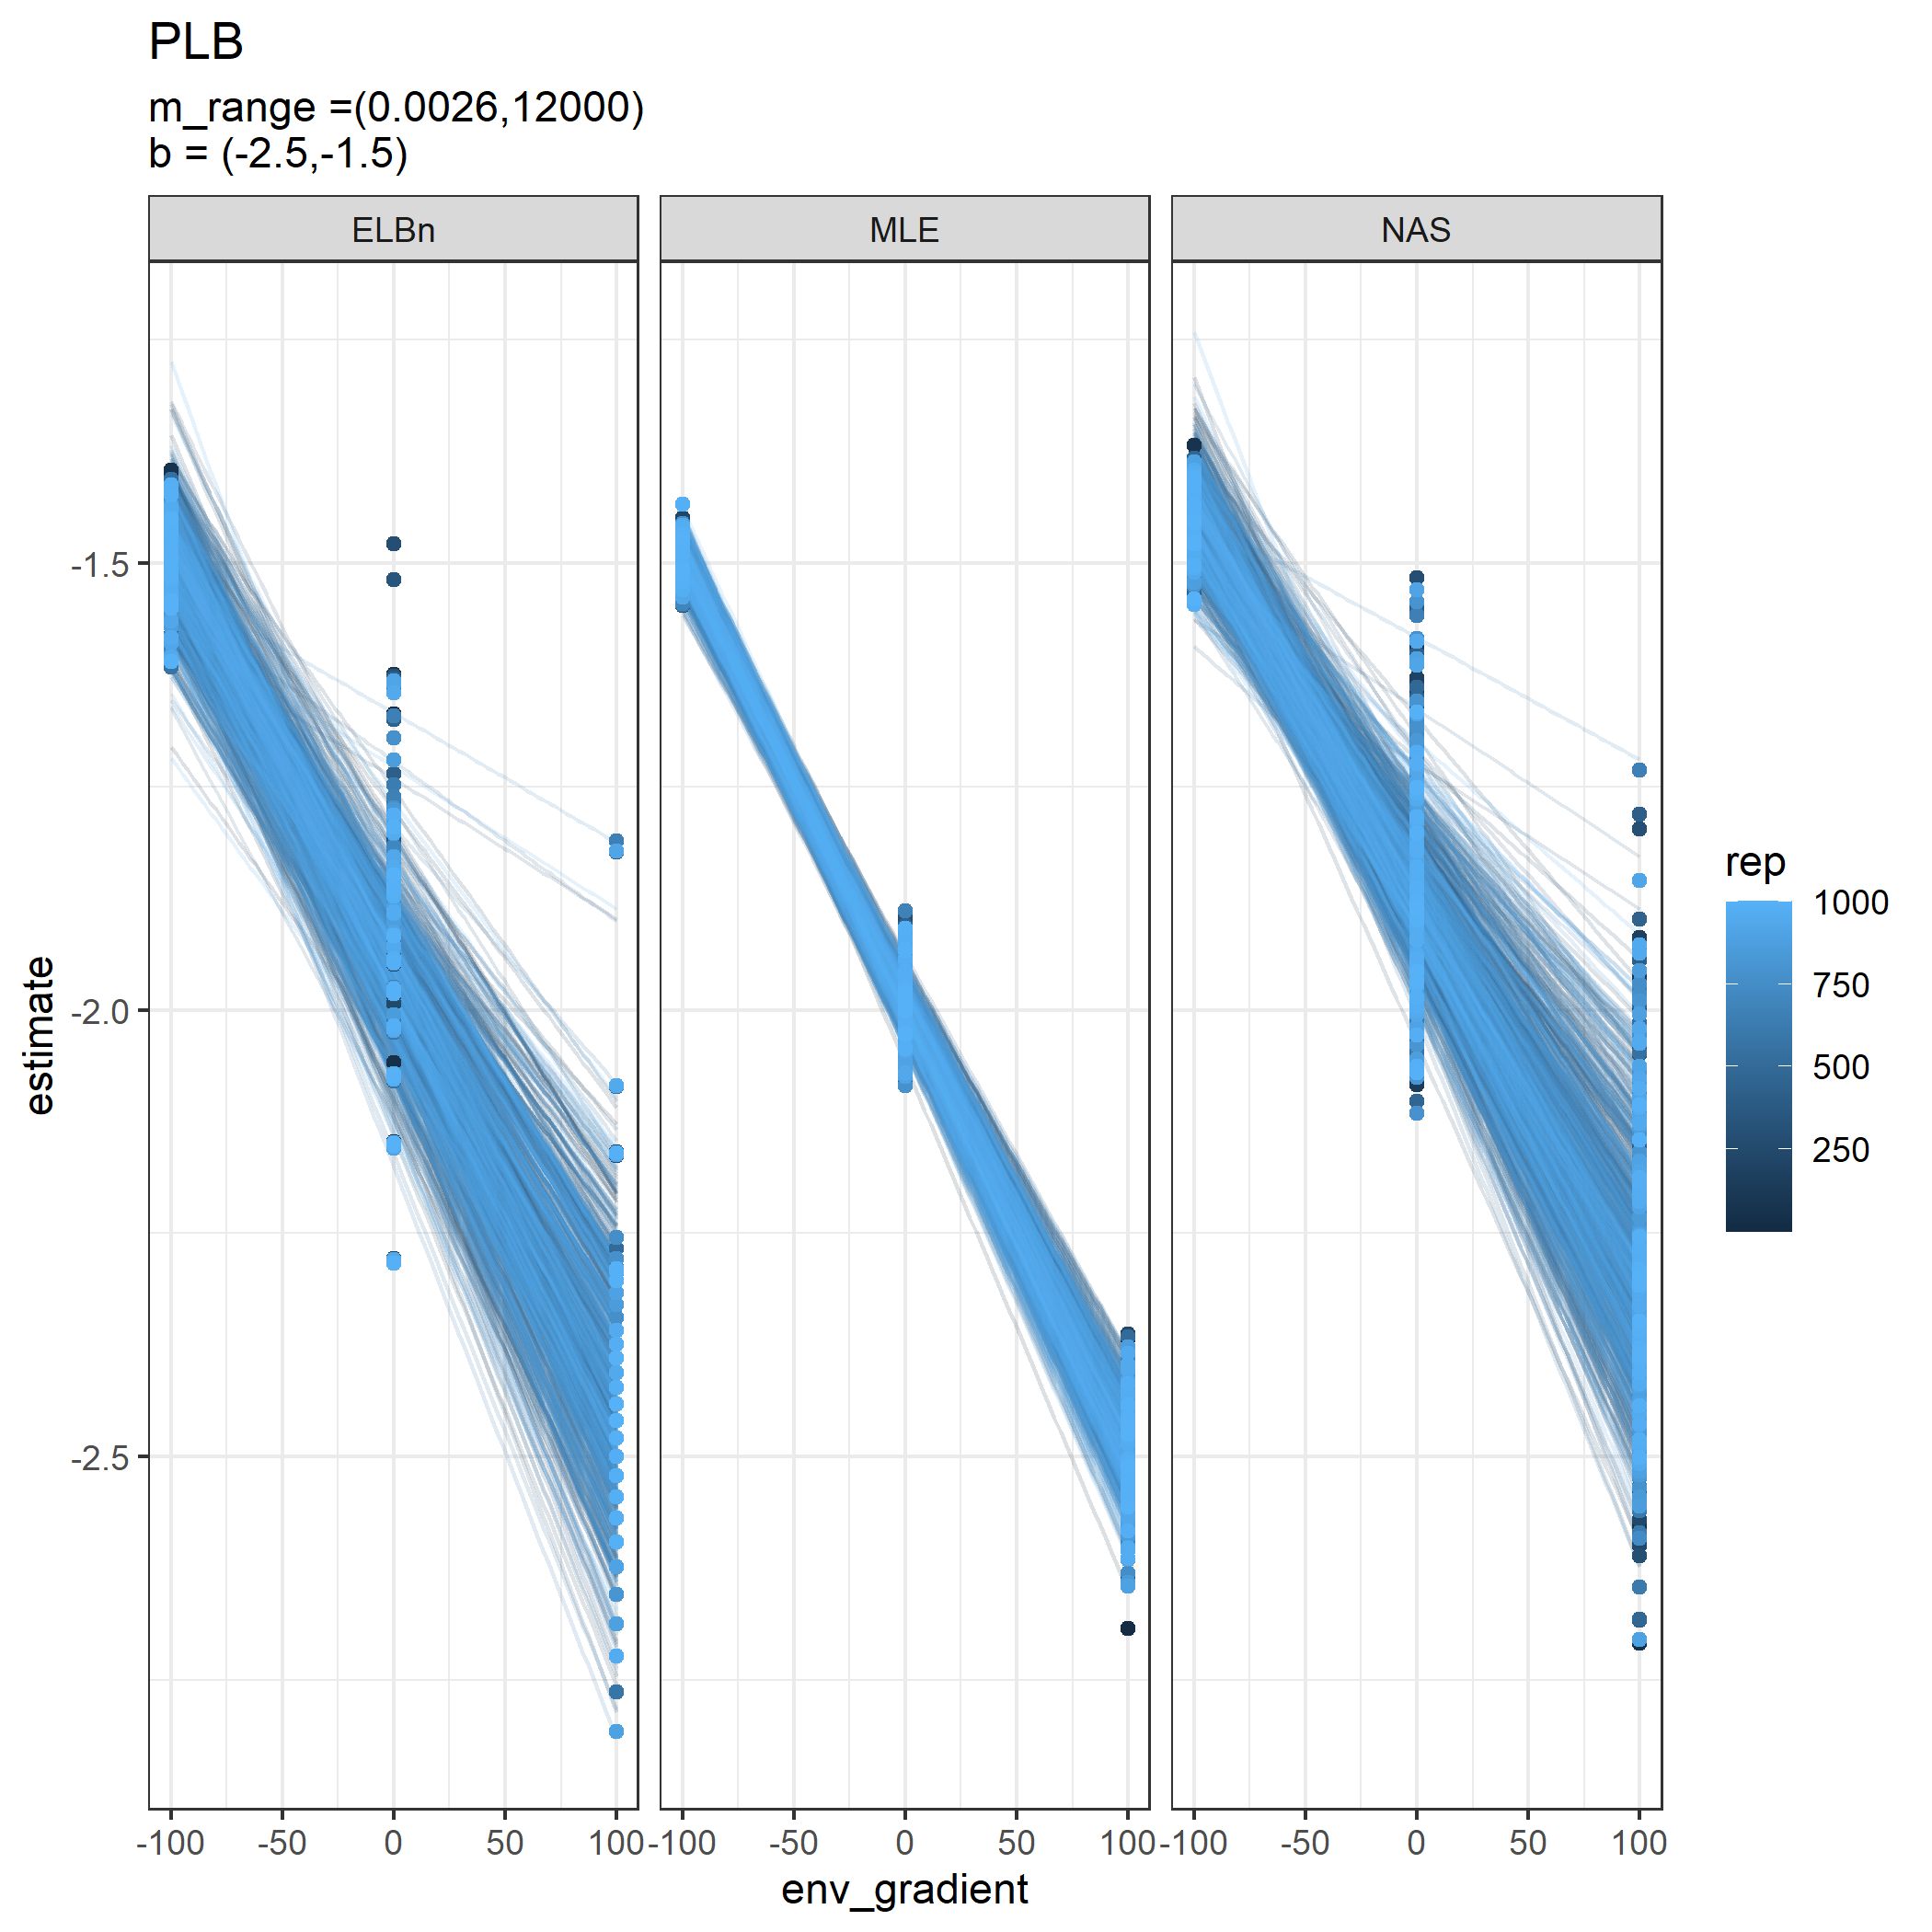
\includegraphics{figures/PLB_large_x_main.png}
\caption{Individual regressions for five sites across a hypothetical
gradient with a known relationship of 0.5. Range of environmental values
(\emph{x}-axis) increased to be -1000, to 1000.}
\end{figure}

\begin{figure}
\centering
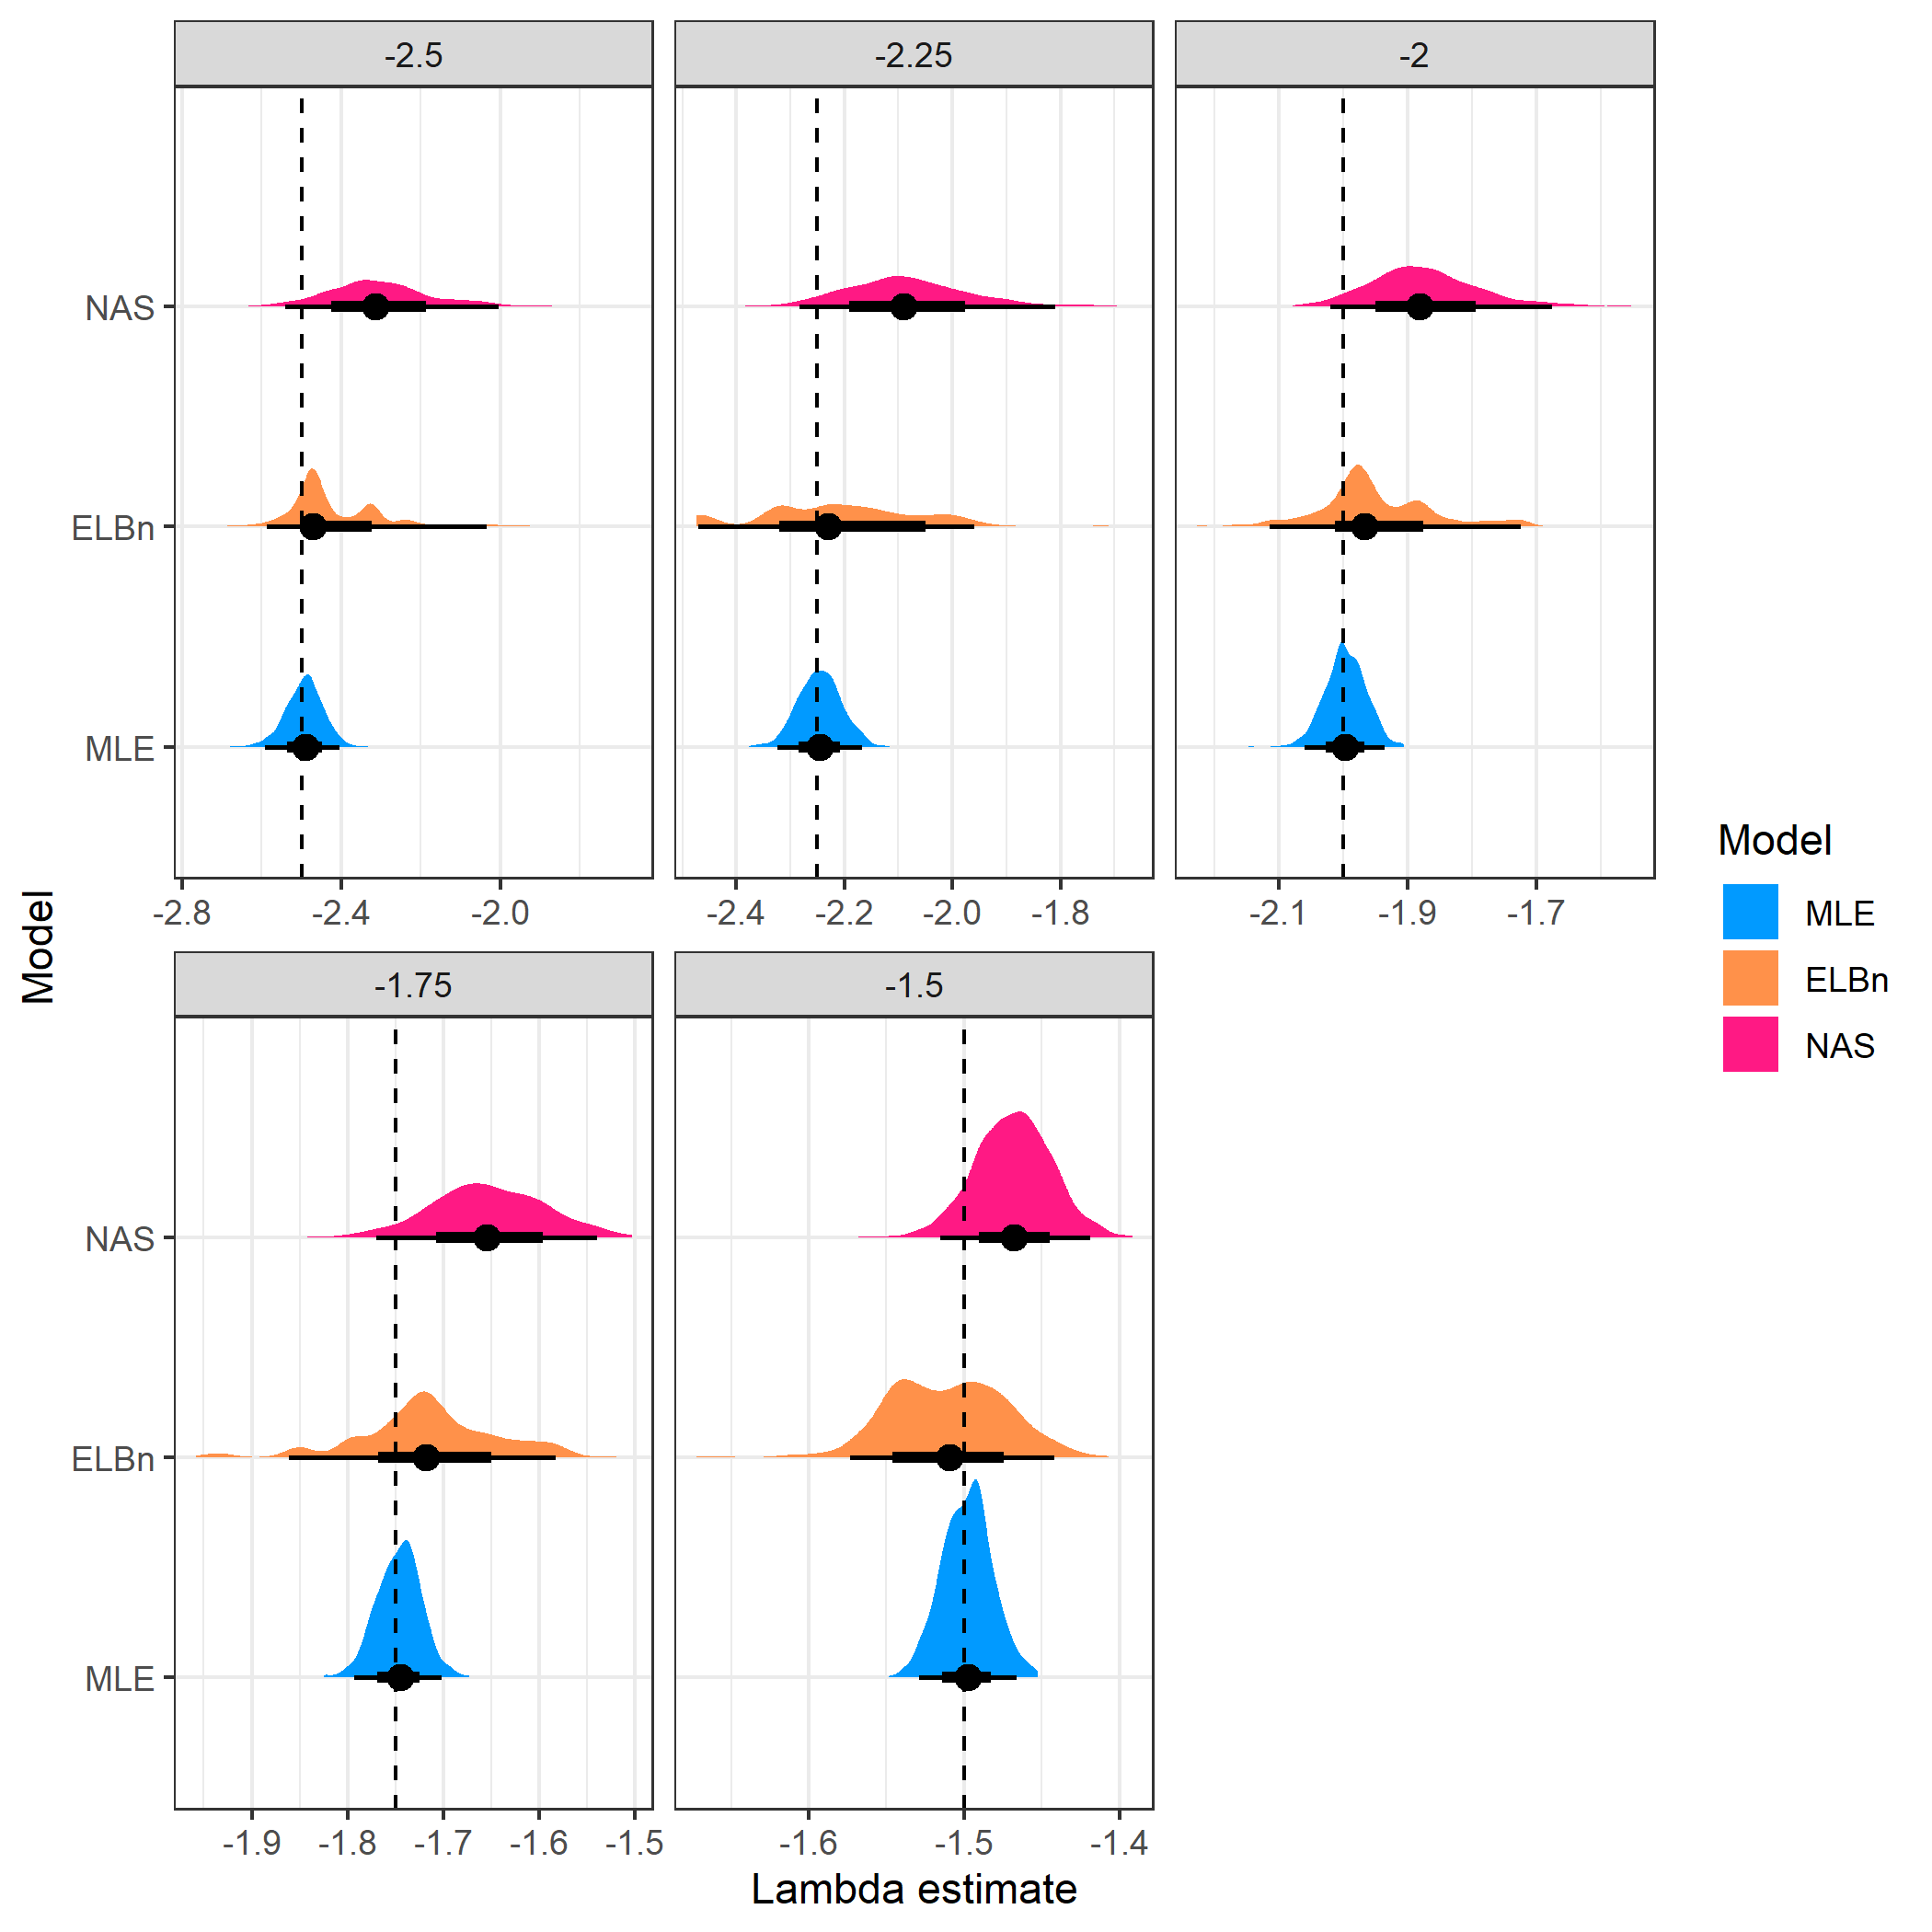
\includegraphics{figures/PLB_large_x_est_b_density.png}
\caption{Distribution of estimated \(\lambda\) coefficient for five
sites across a hypothetical gradient with known values. Range of
environmental values (\emph{x}-axis) increased to be -1000, to 1000.}
\end{figure}

\begin{figure}
\centering
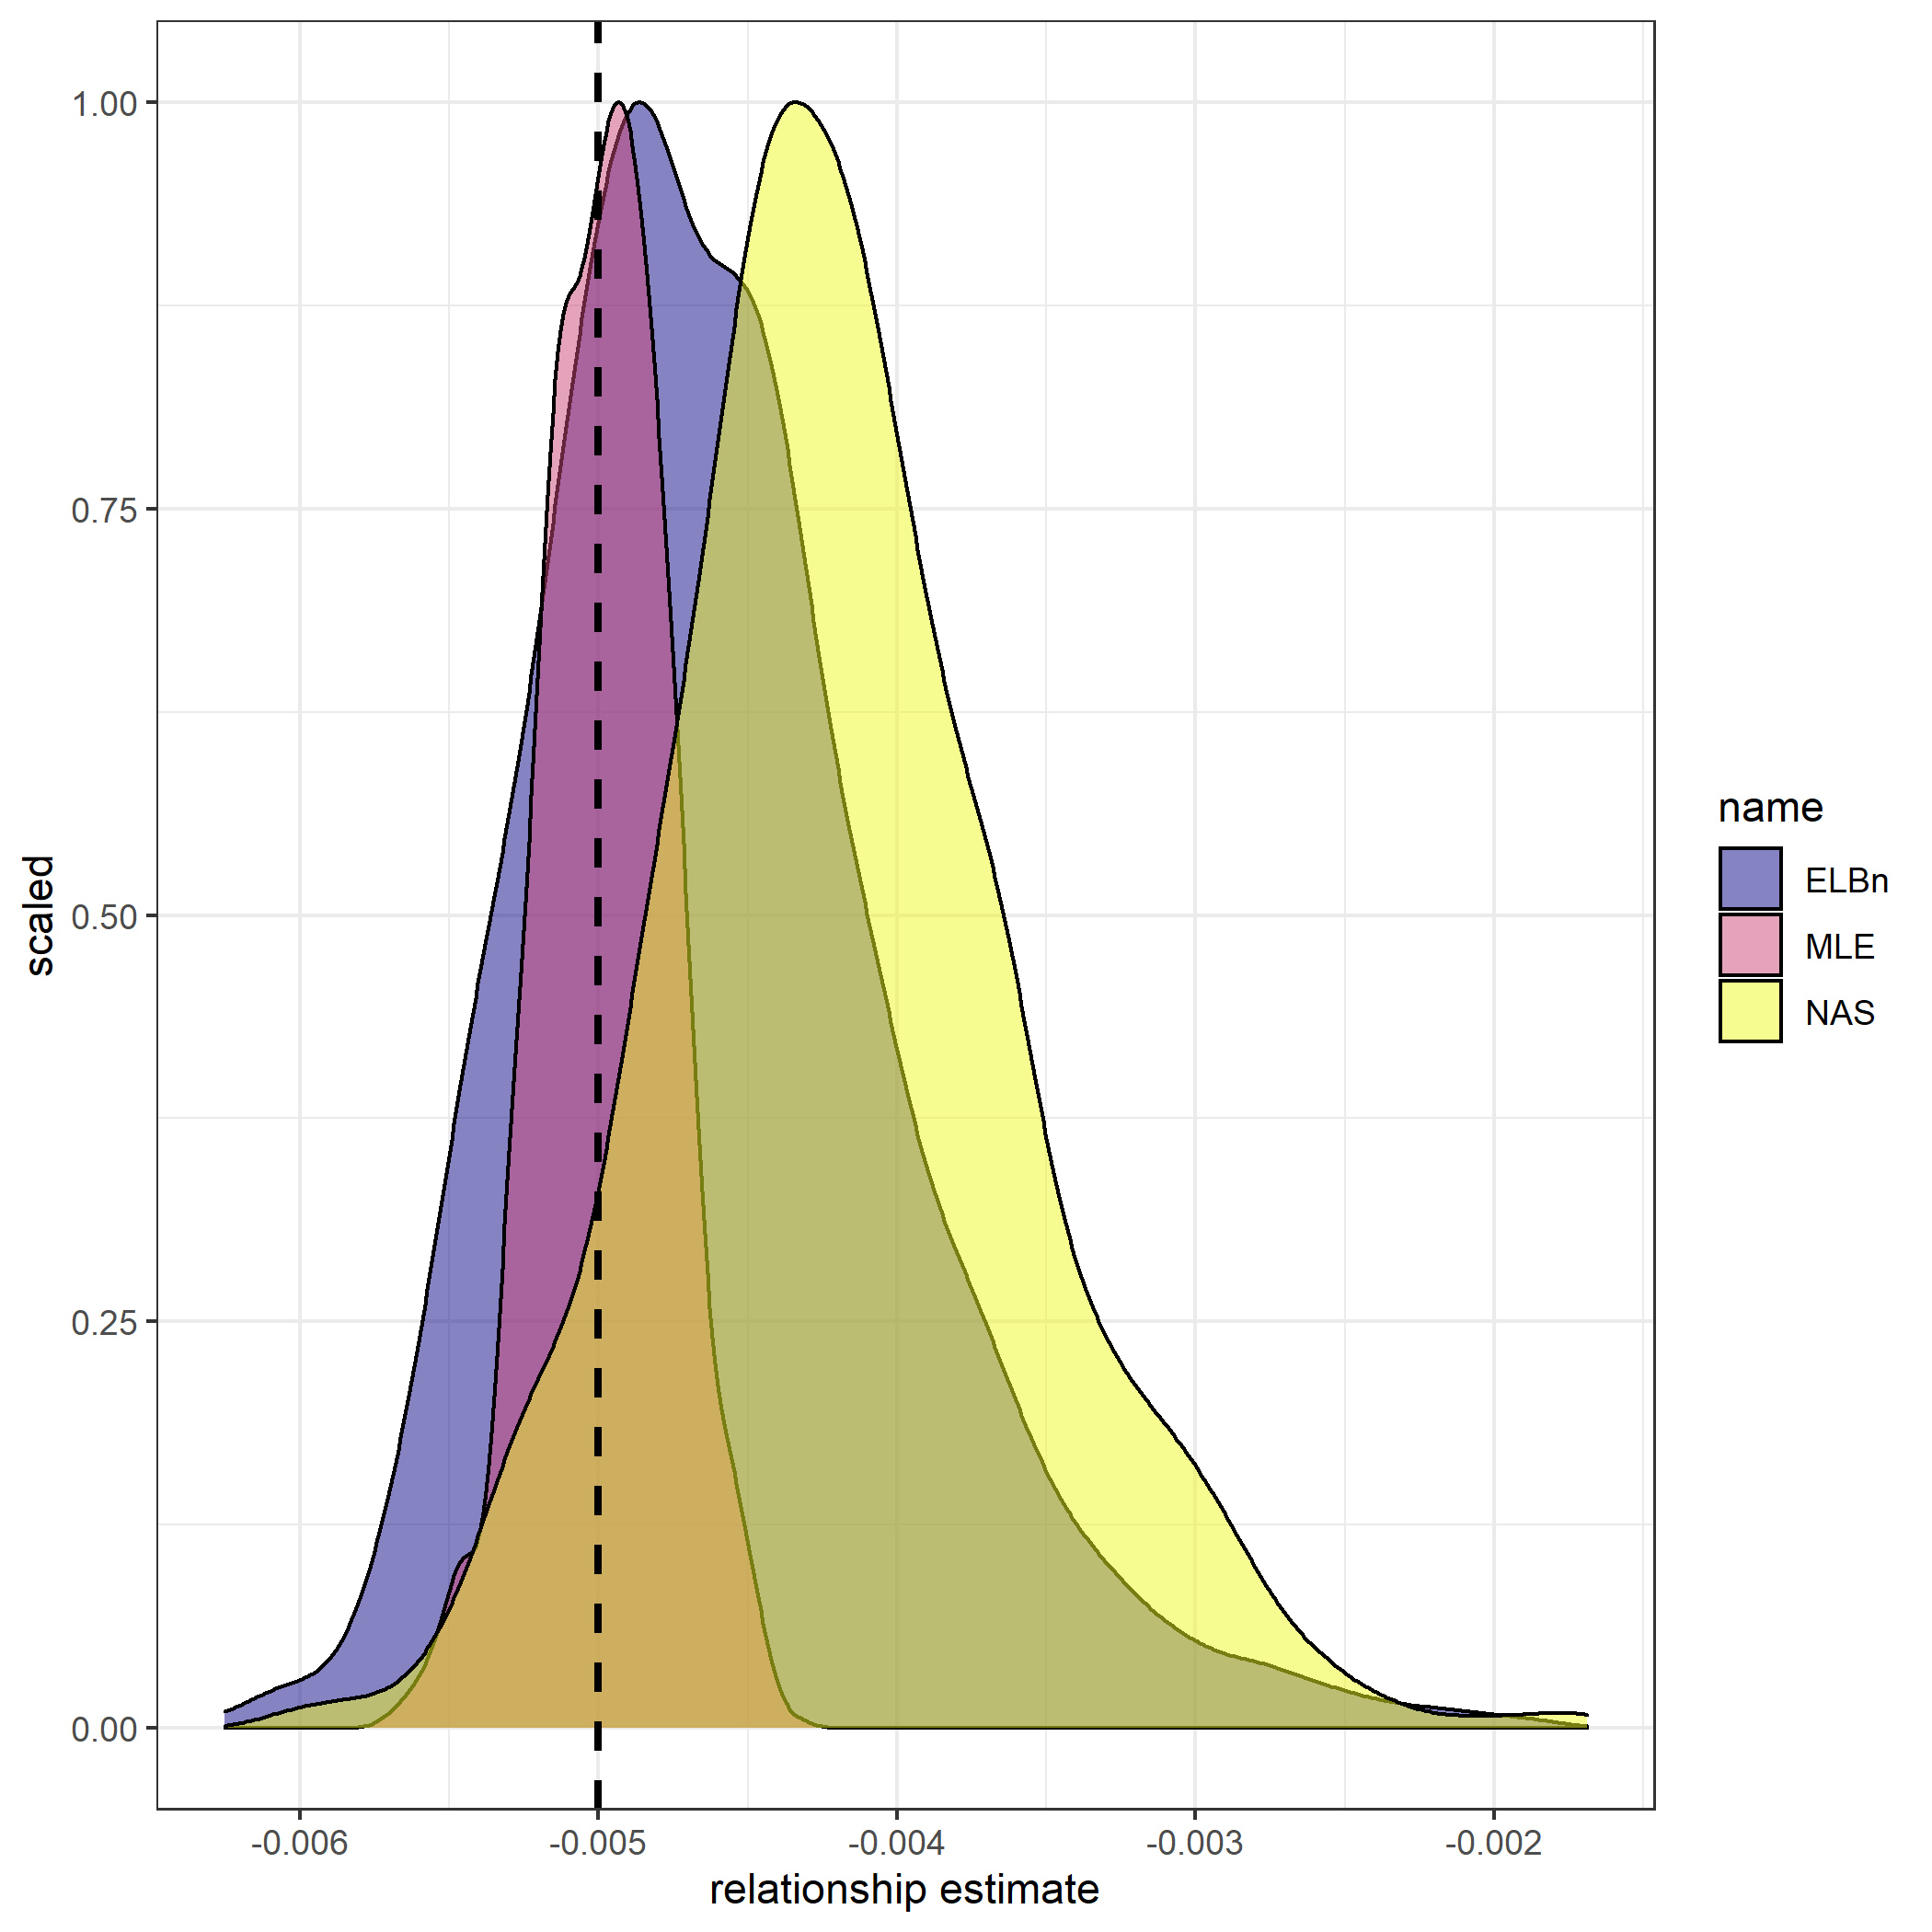
\includegraphics{figures/PLB_large_x_relationship_density.png}
\caption{Distribution of estimated relationship (\(\beta_1\))
coefficient's for five sites across a hypothetical gradient with known
value of 0.5. Range of environmental values (\emph{x}-axis) increased to
be -1000, to 1000.}
\end{figure}

\hypertarget{varying-number-of-sites}{%
\subsection{Varying number of sites}\label{varying-number-of-sites}}

\hypertarget{sites}{%
\subsubsection{10 sites}\label{sites}}

\begin{figure}
\centering
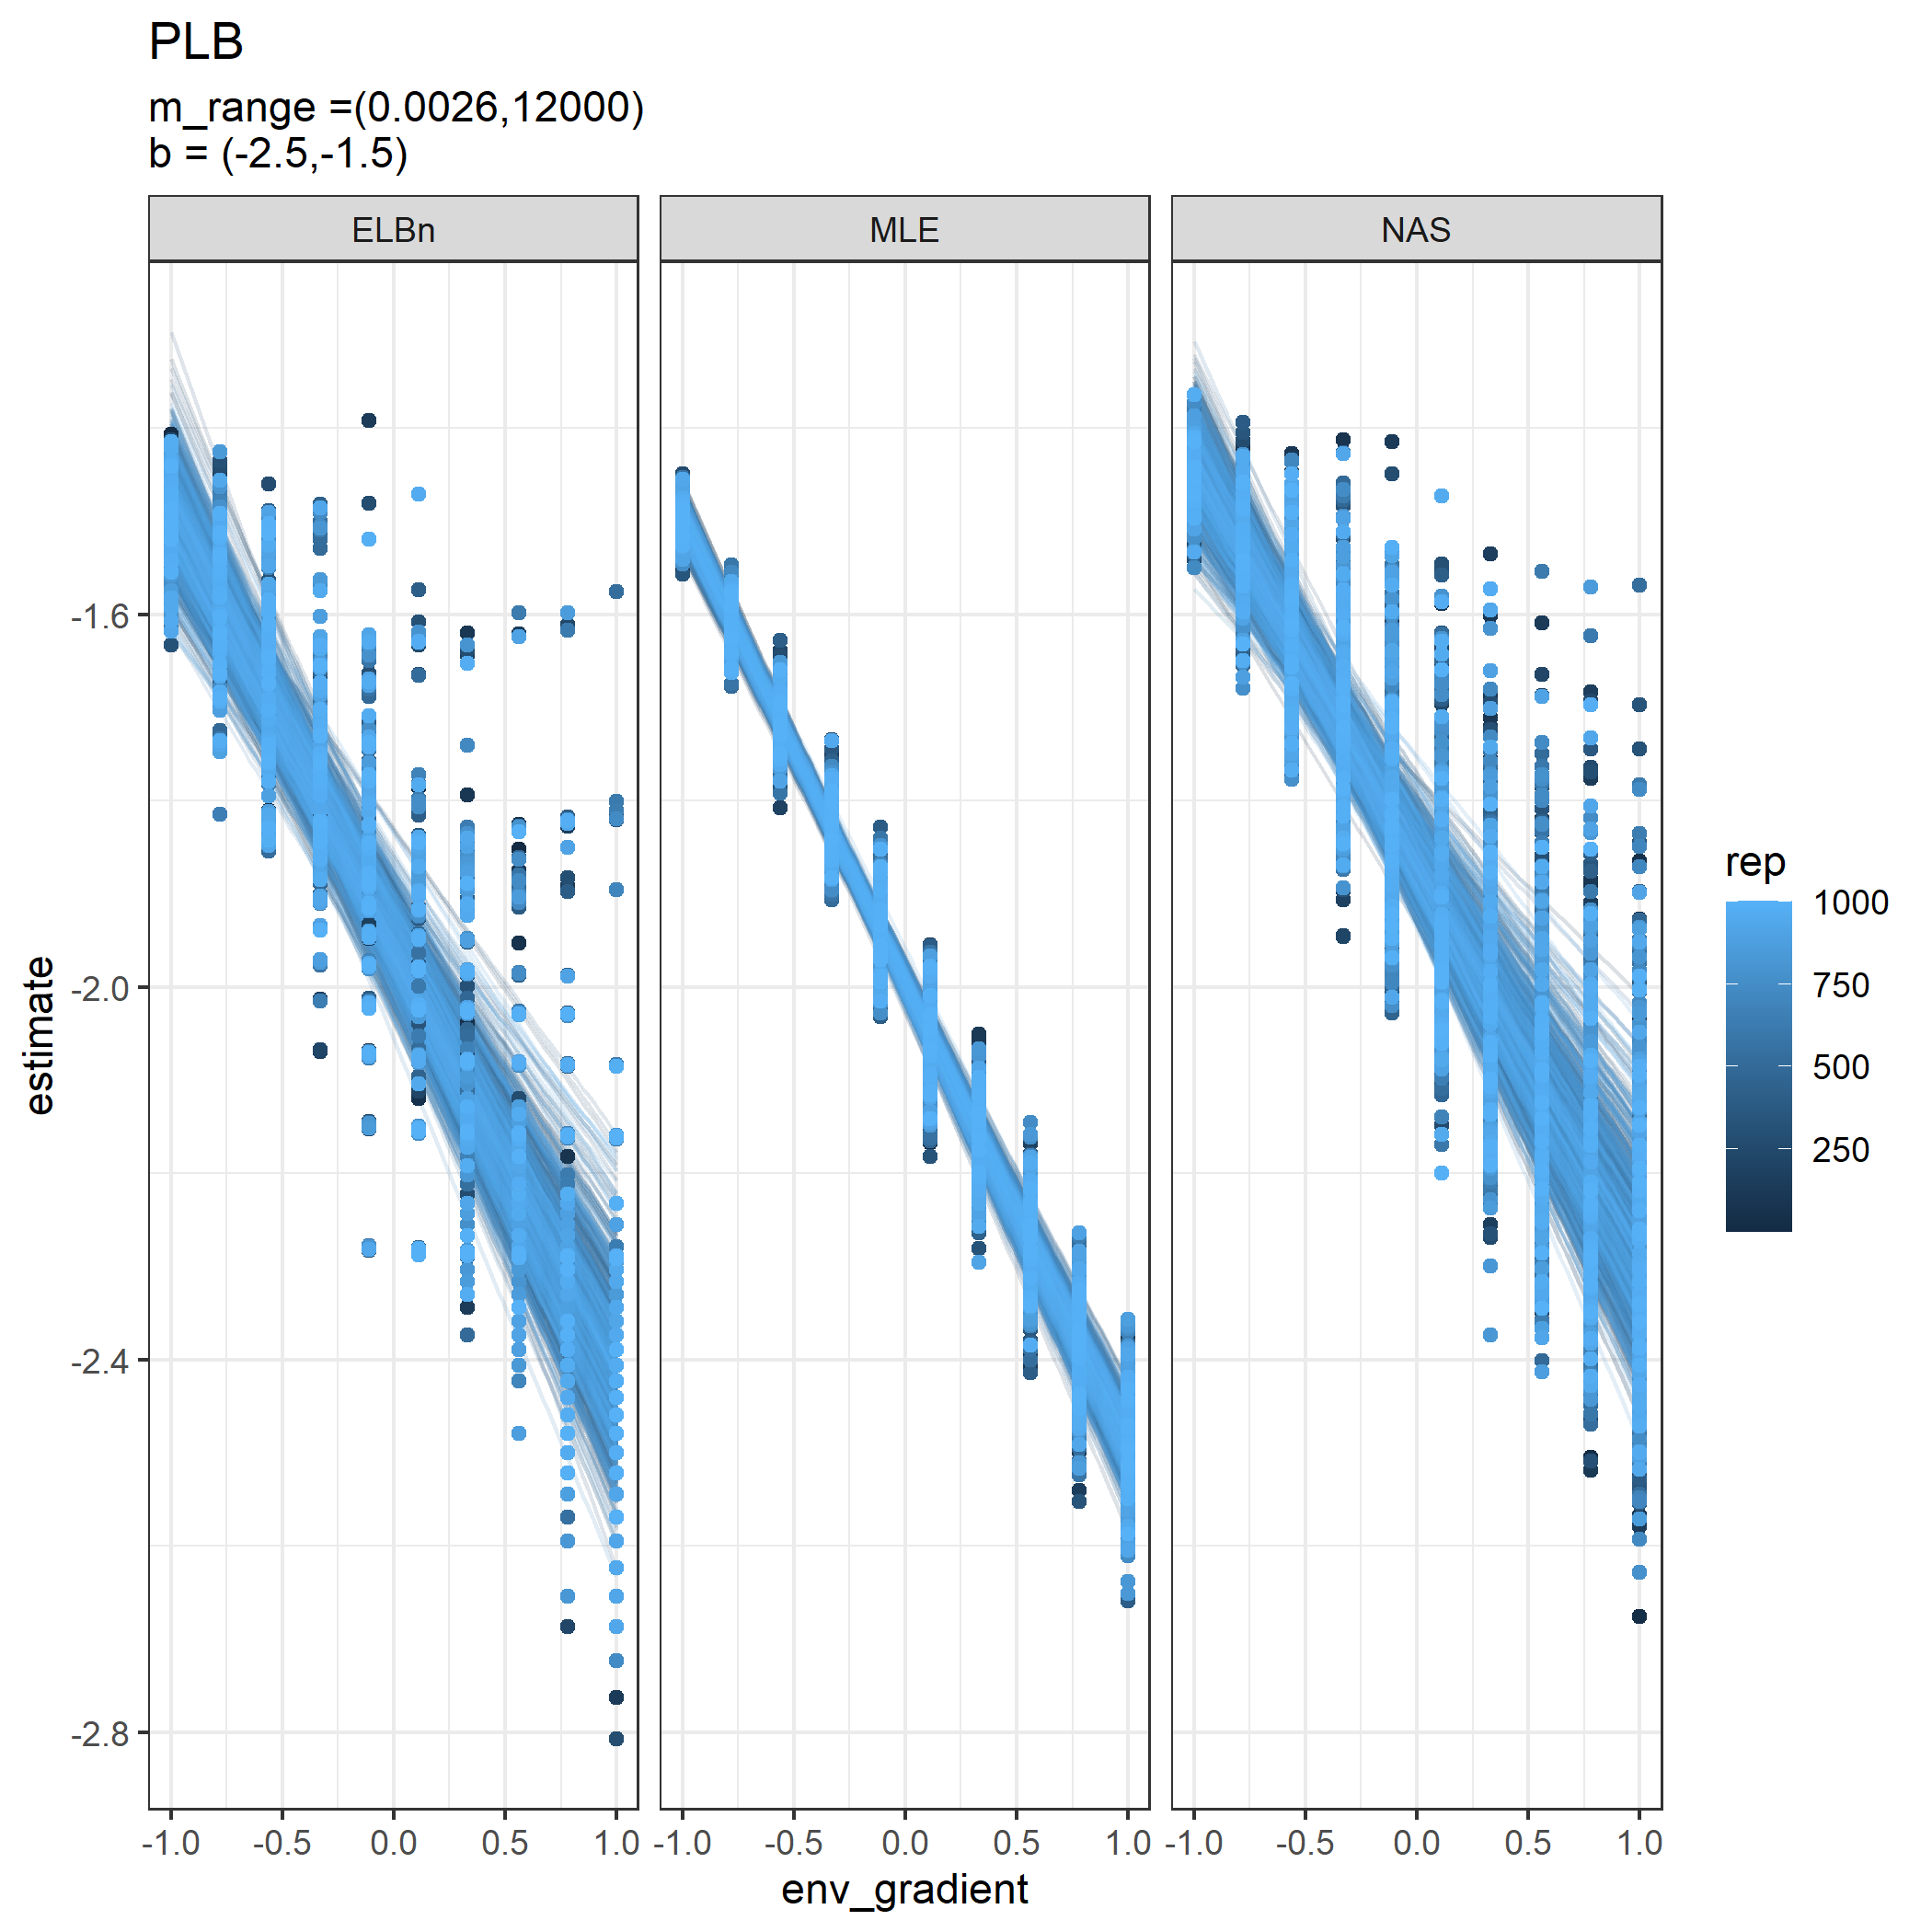
\includegraphics{figures/PLB_10_sites_main.png}
\caption{Individual regressions for ten sites across a hypothetical
gradient with a known relationship of 0.5. All other parameters are the
same as in the main analysis}
\end{figure}

\begin{figure}
\centering
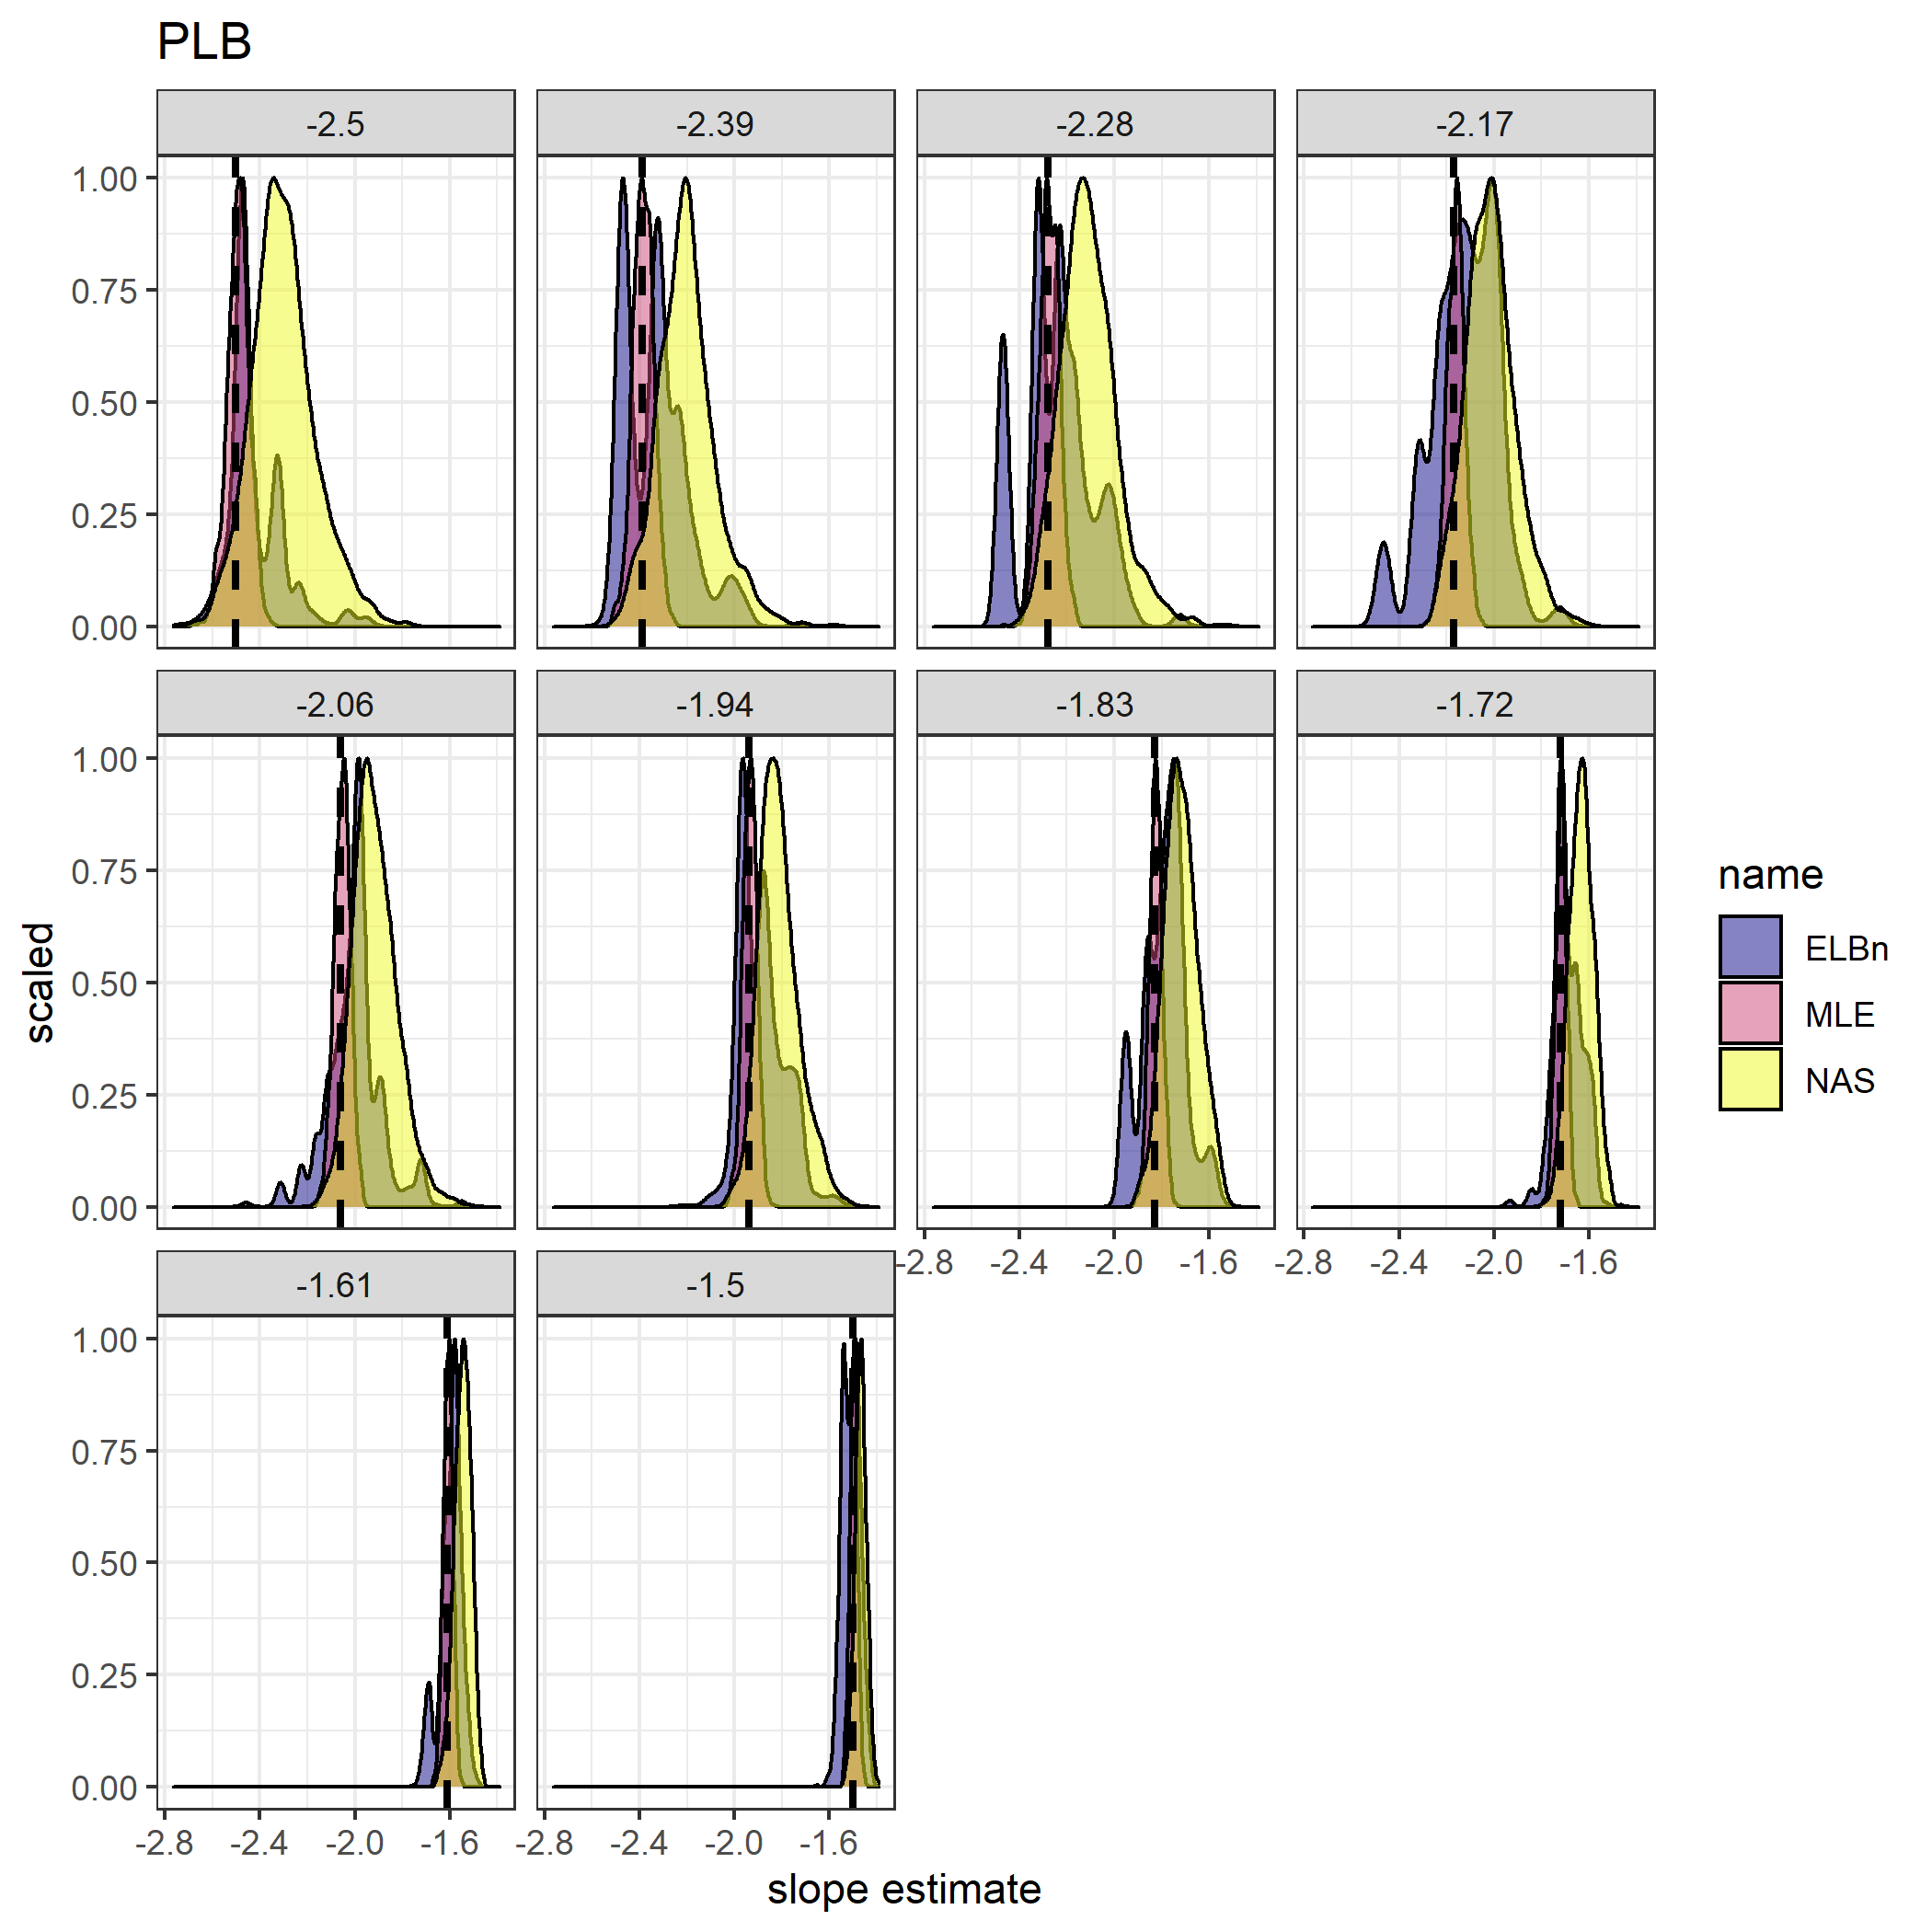
\includegraphics{figures/PLB_10_sites_est_b_density.png}
\caption{Distribution of estimated \(\lambda\) coefficient for ten sites
across a hypothetical gradient with known values. All other parameters
are the same as in the main analysis}
\end{figure}

\begin{figure}
\centering
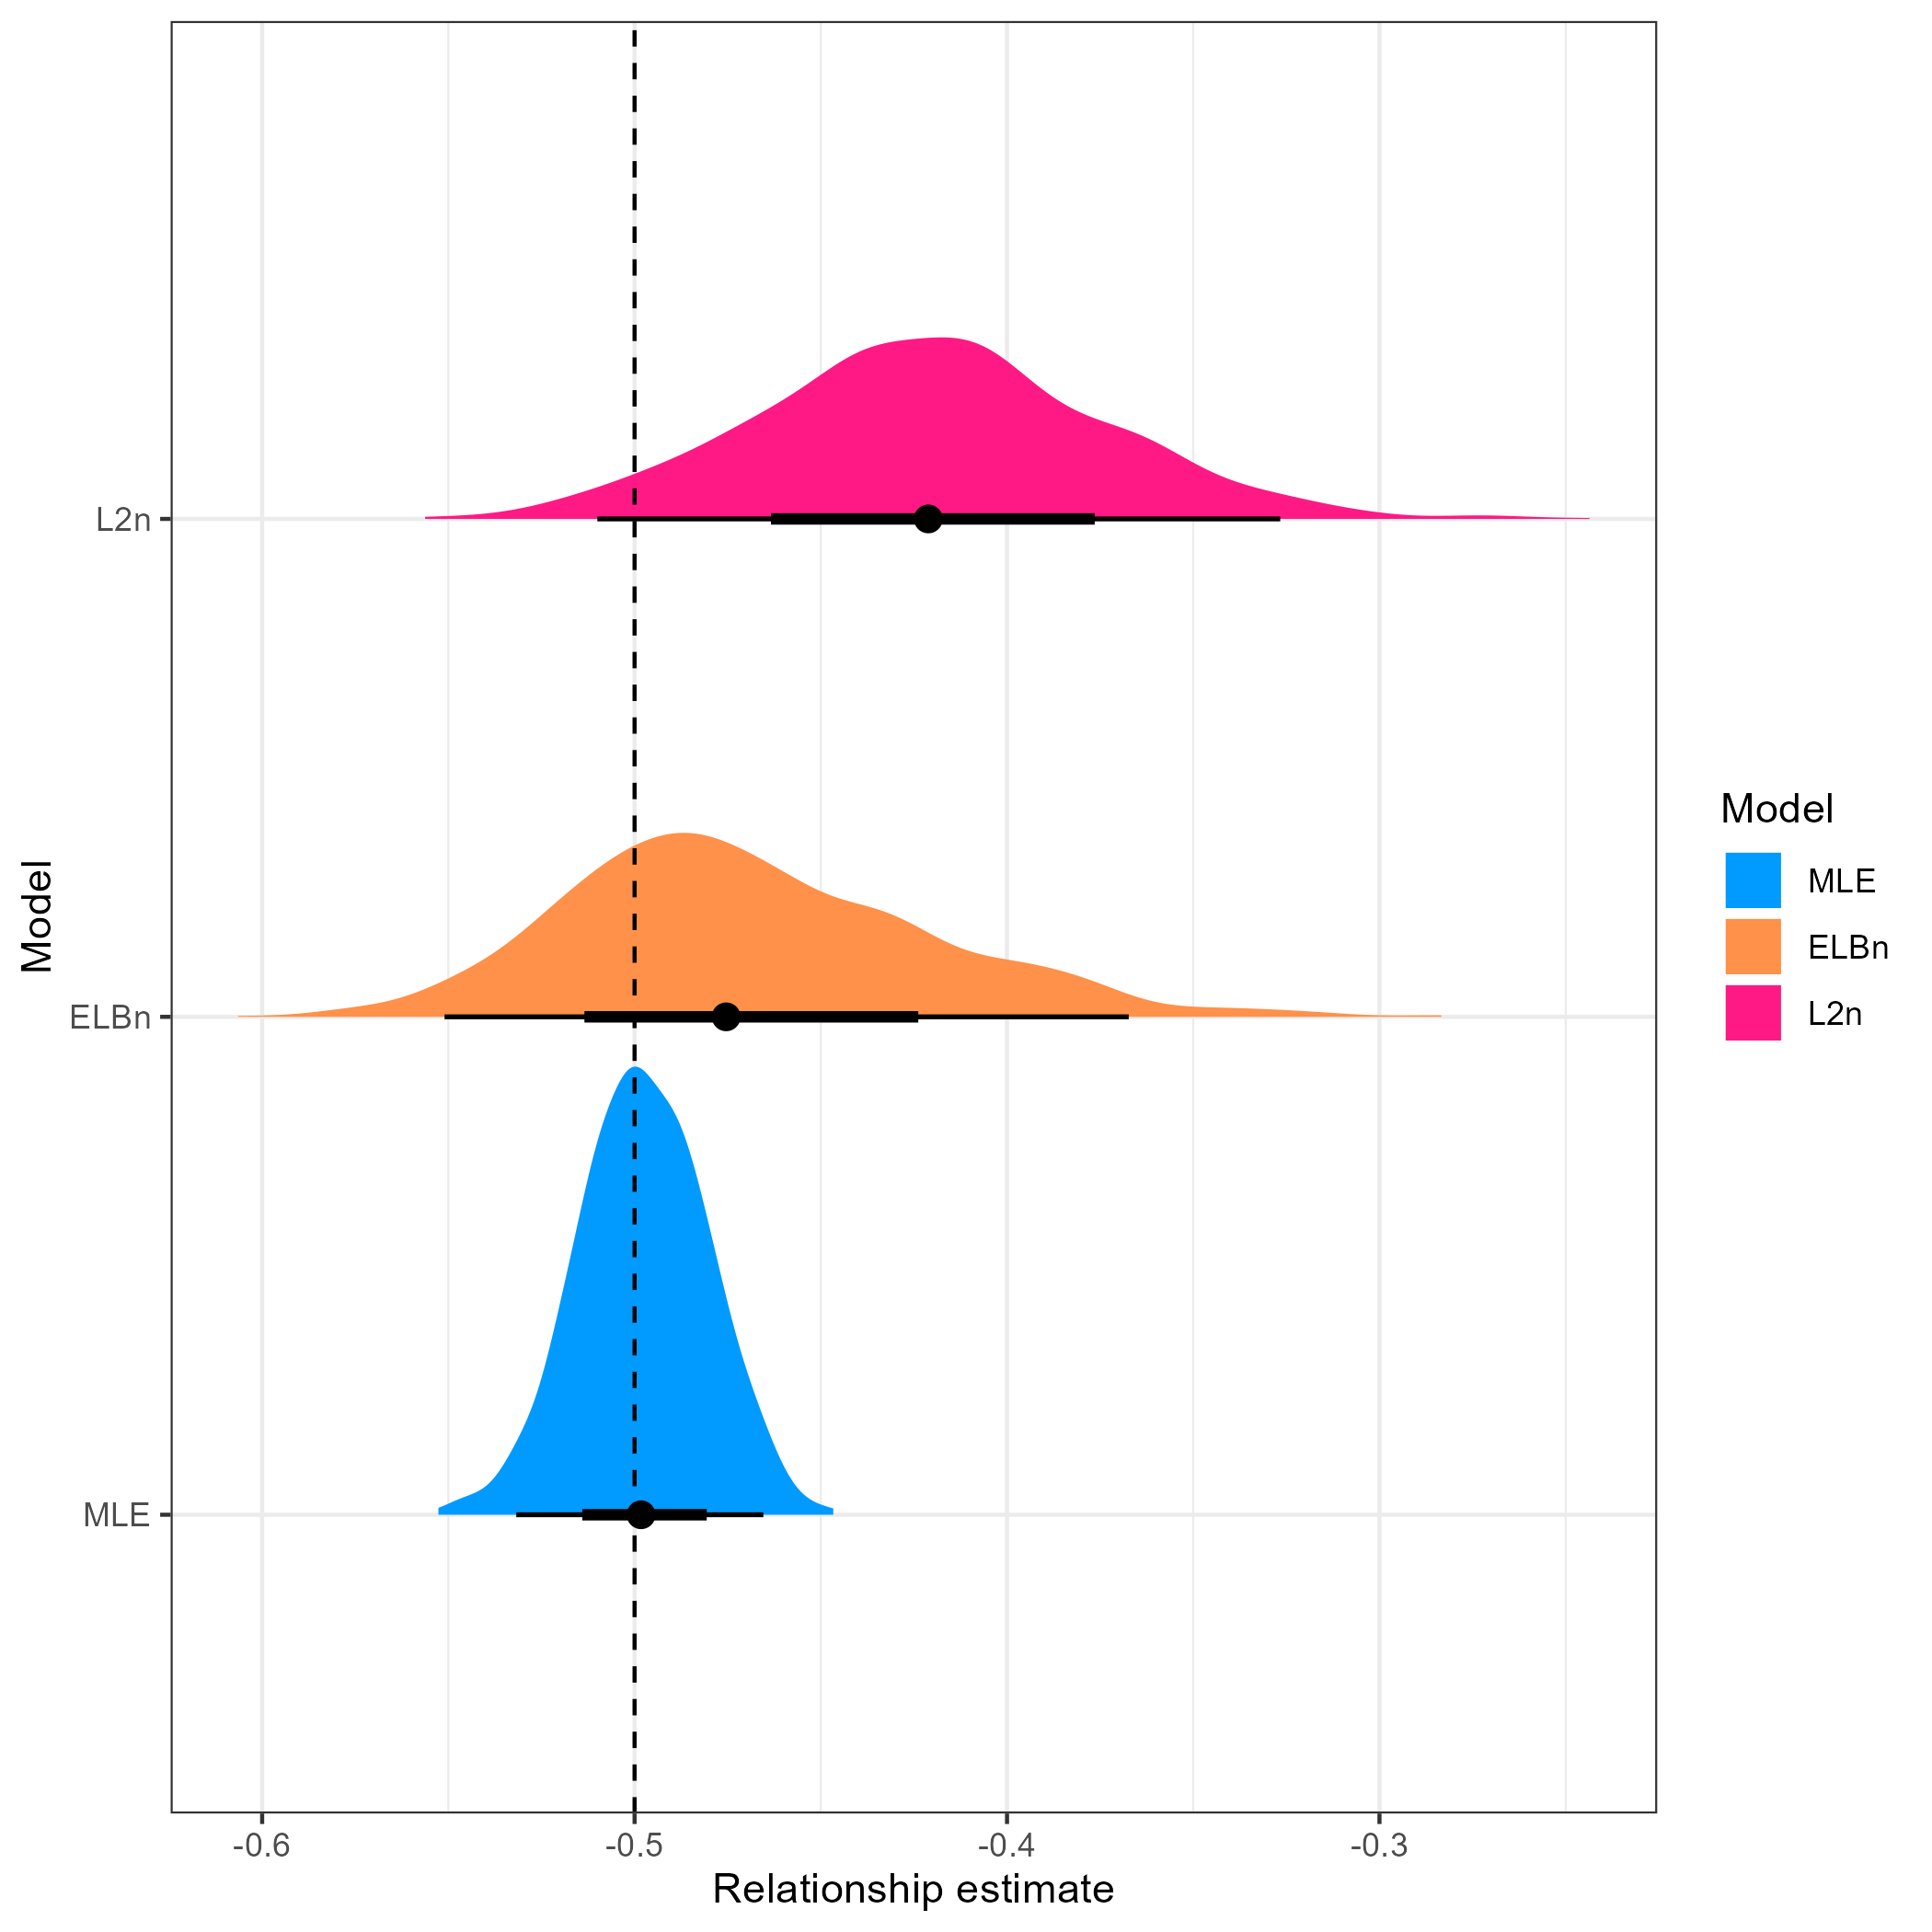
\includegraphics{figures/PLB_10_sites_relationship_density.png}
\caption{Distribution of estimated relationship (\(\beta_1\))
coefficient's for ten sites across a hypothetical gradient with known
value of 0.5. All other parameters are the same as in the main analysis}
\end{figure}

\hypertarget{three-sites}{%
\subsubsection{Three sites}\label{three-sites}}

\begin{figure}
\centering
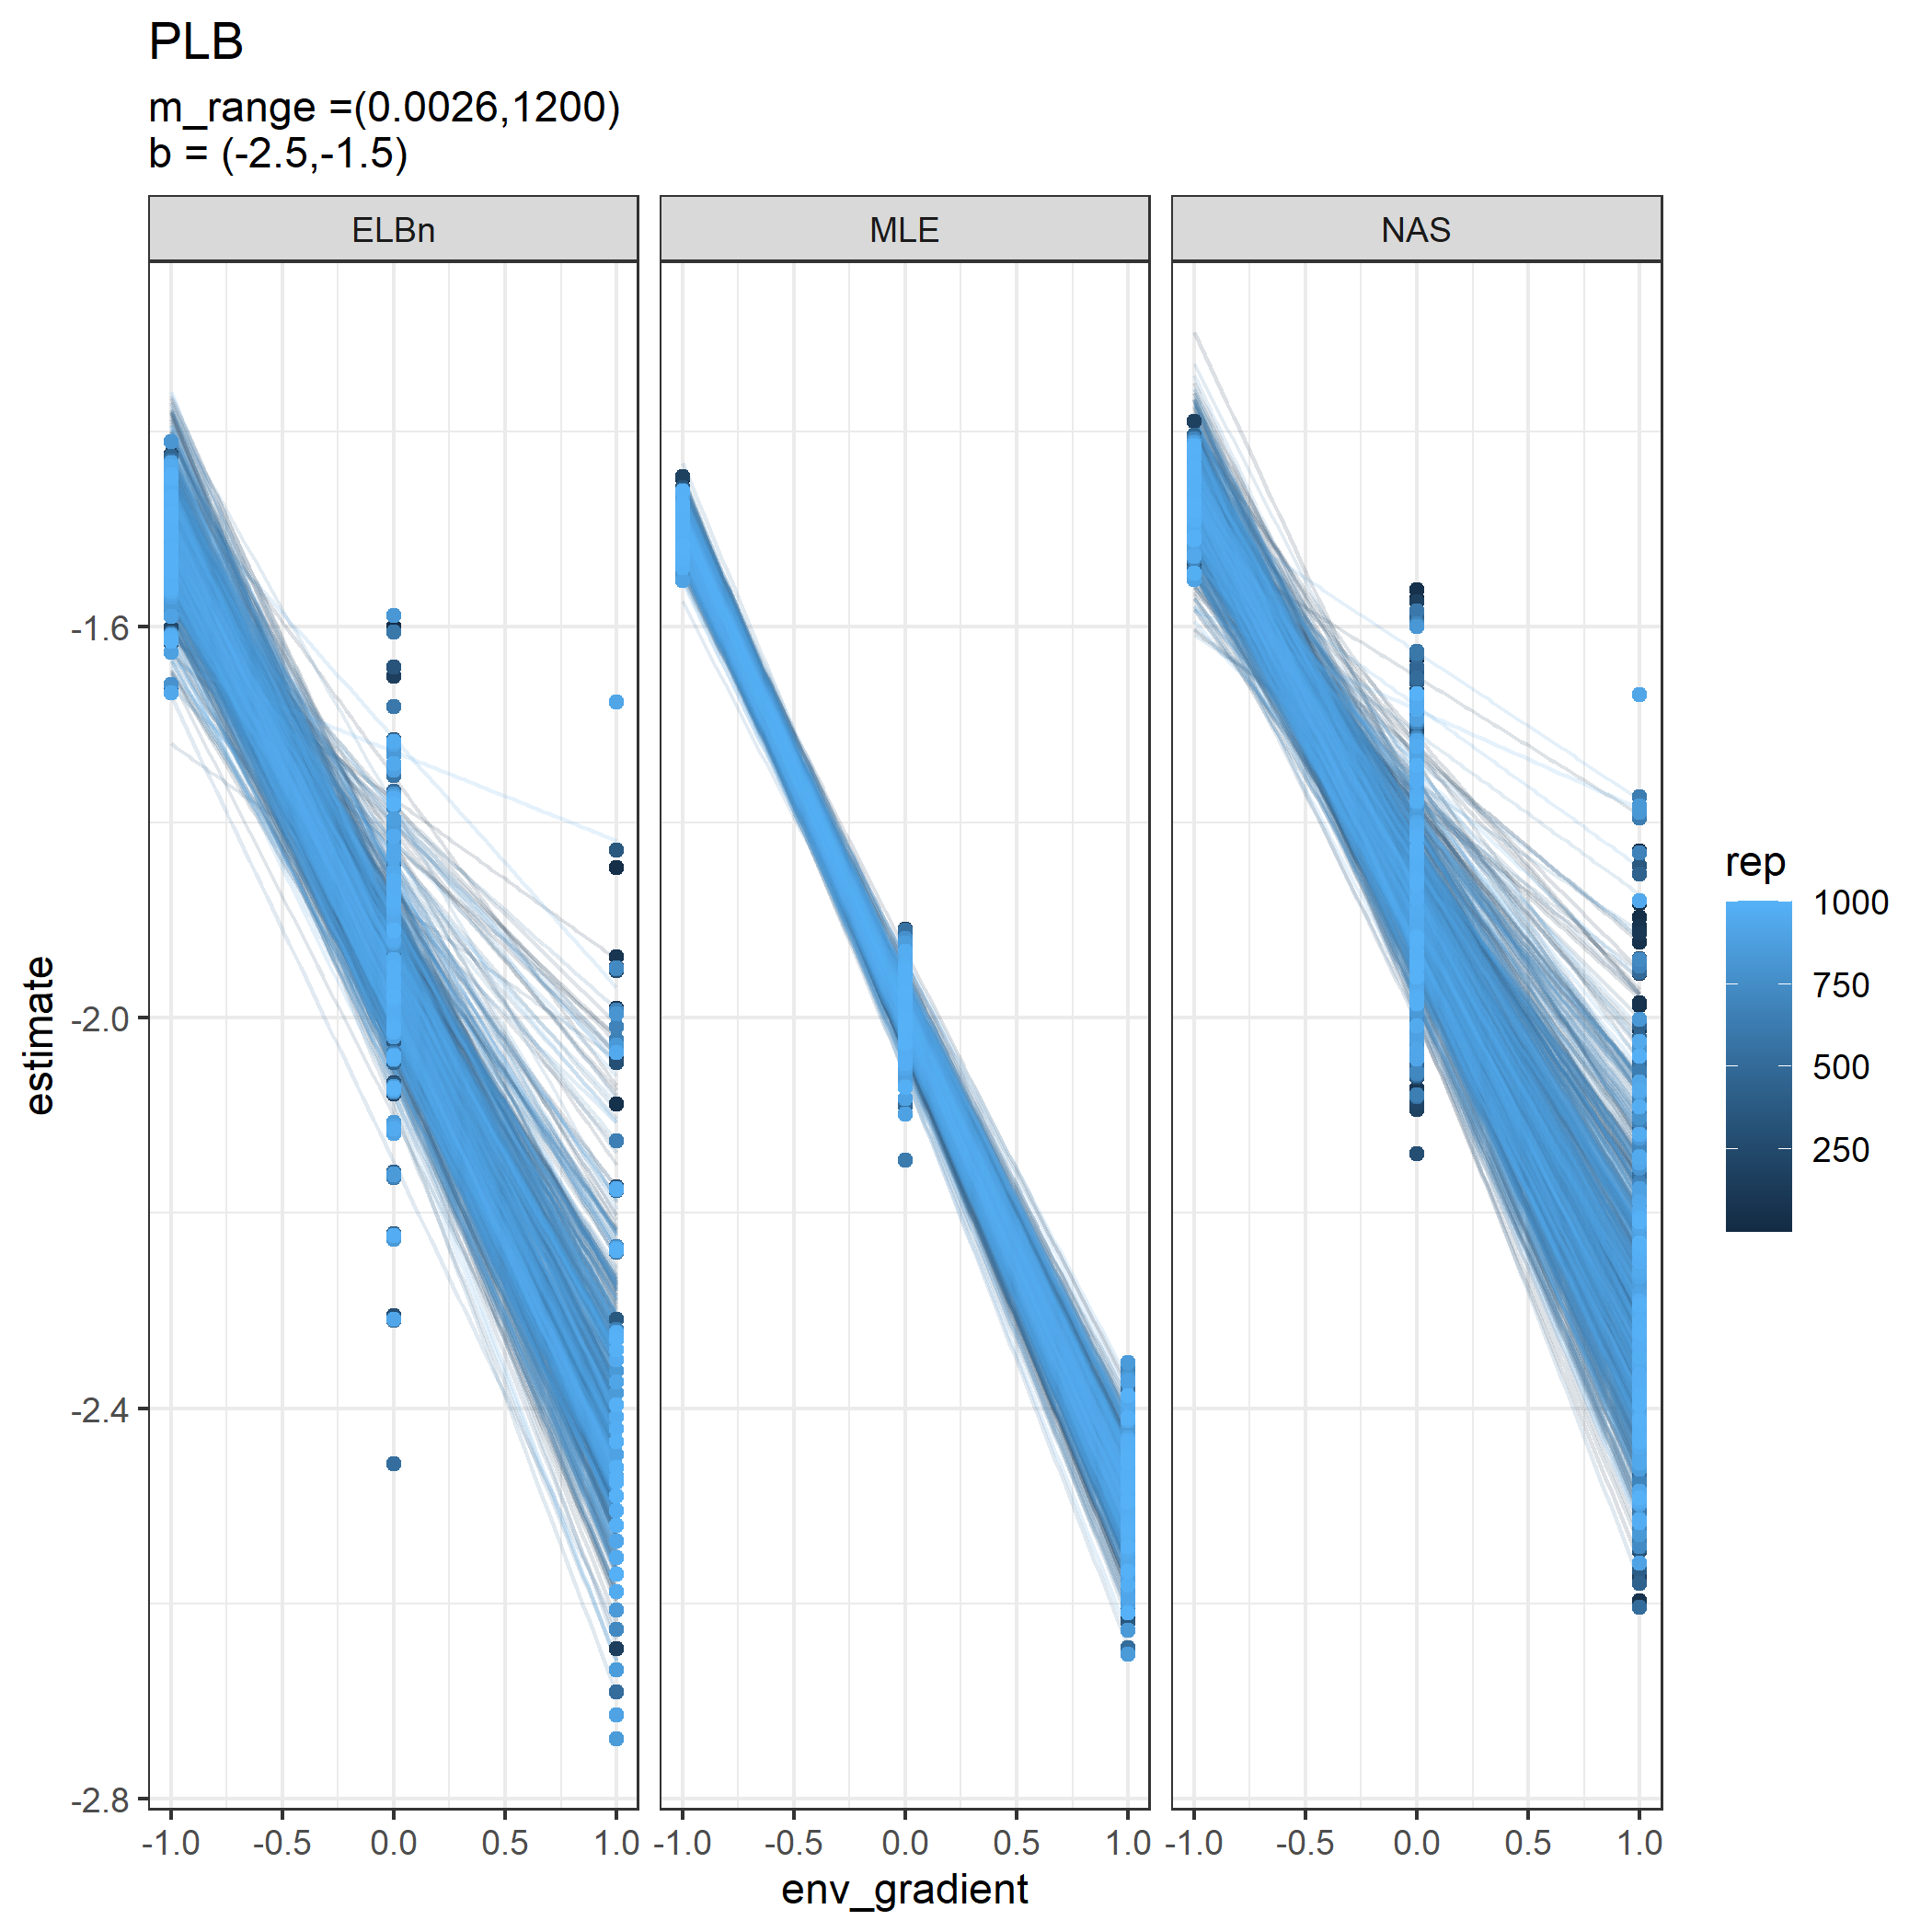
\includegraphics{figures/PLB_3_sites_main.png}
\caption{Individual regressions for three sites across a hypothetical
gradient with a known relationship of 0.5. All other parameters are the
same as in the main analysis.}
\end{figure}

\begin{figure}
\centering
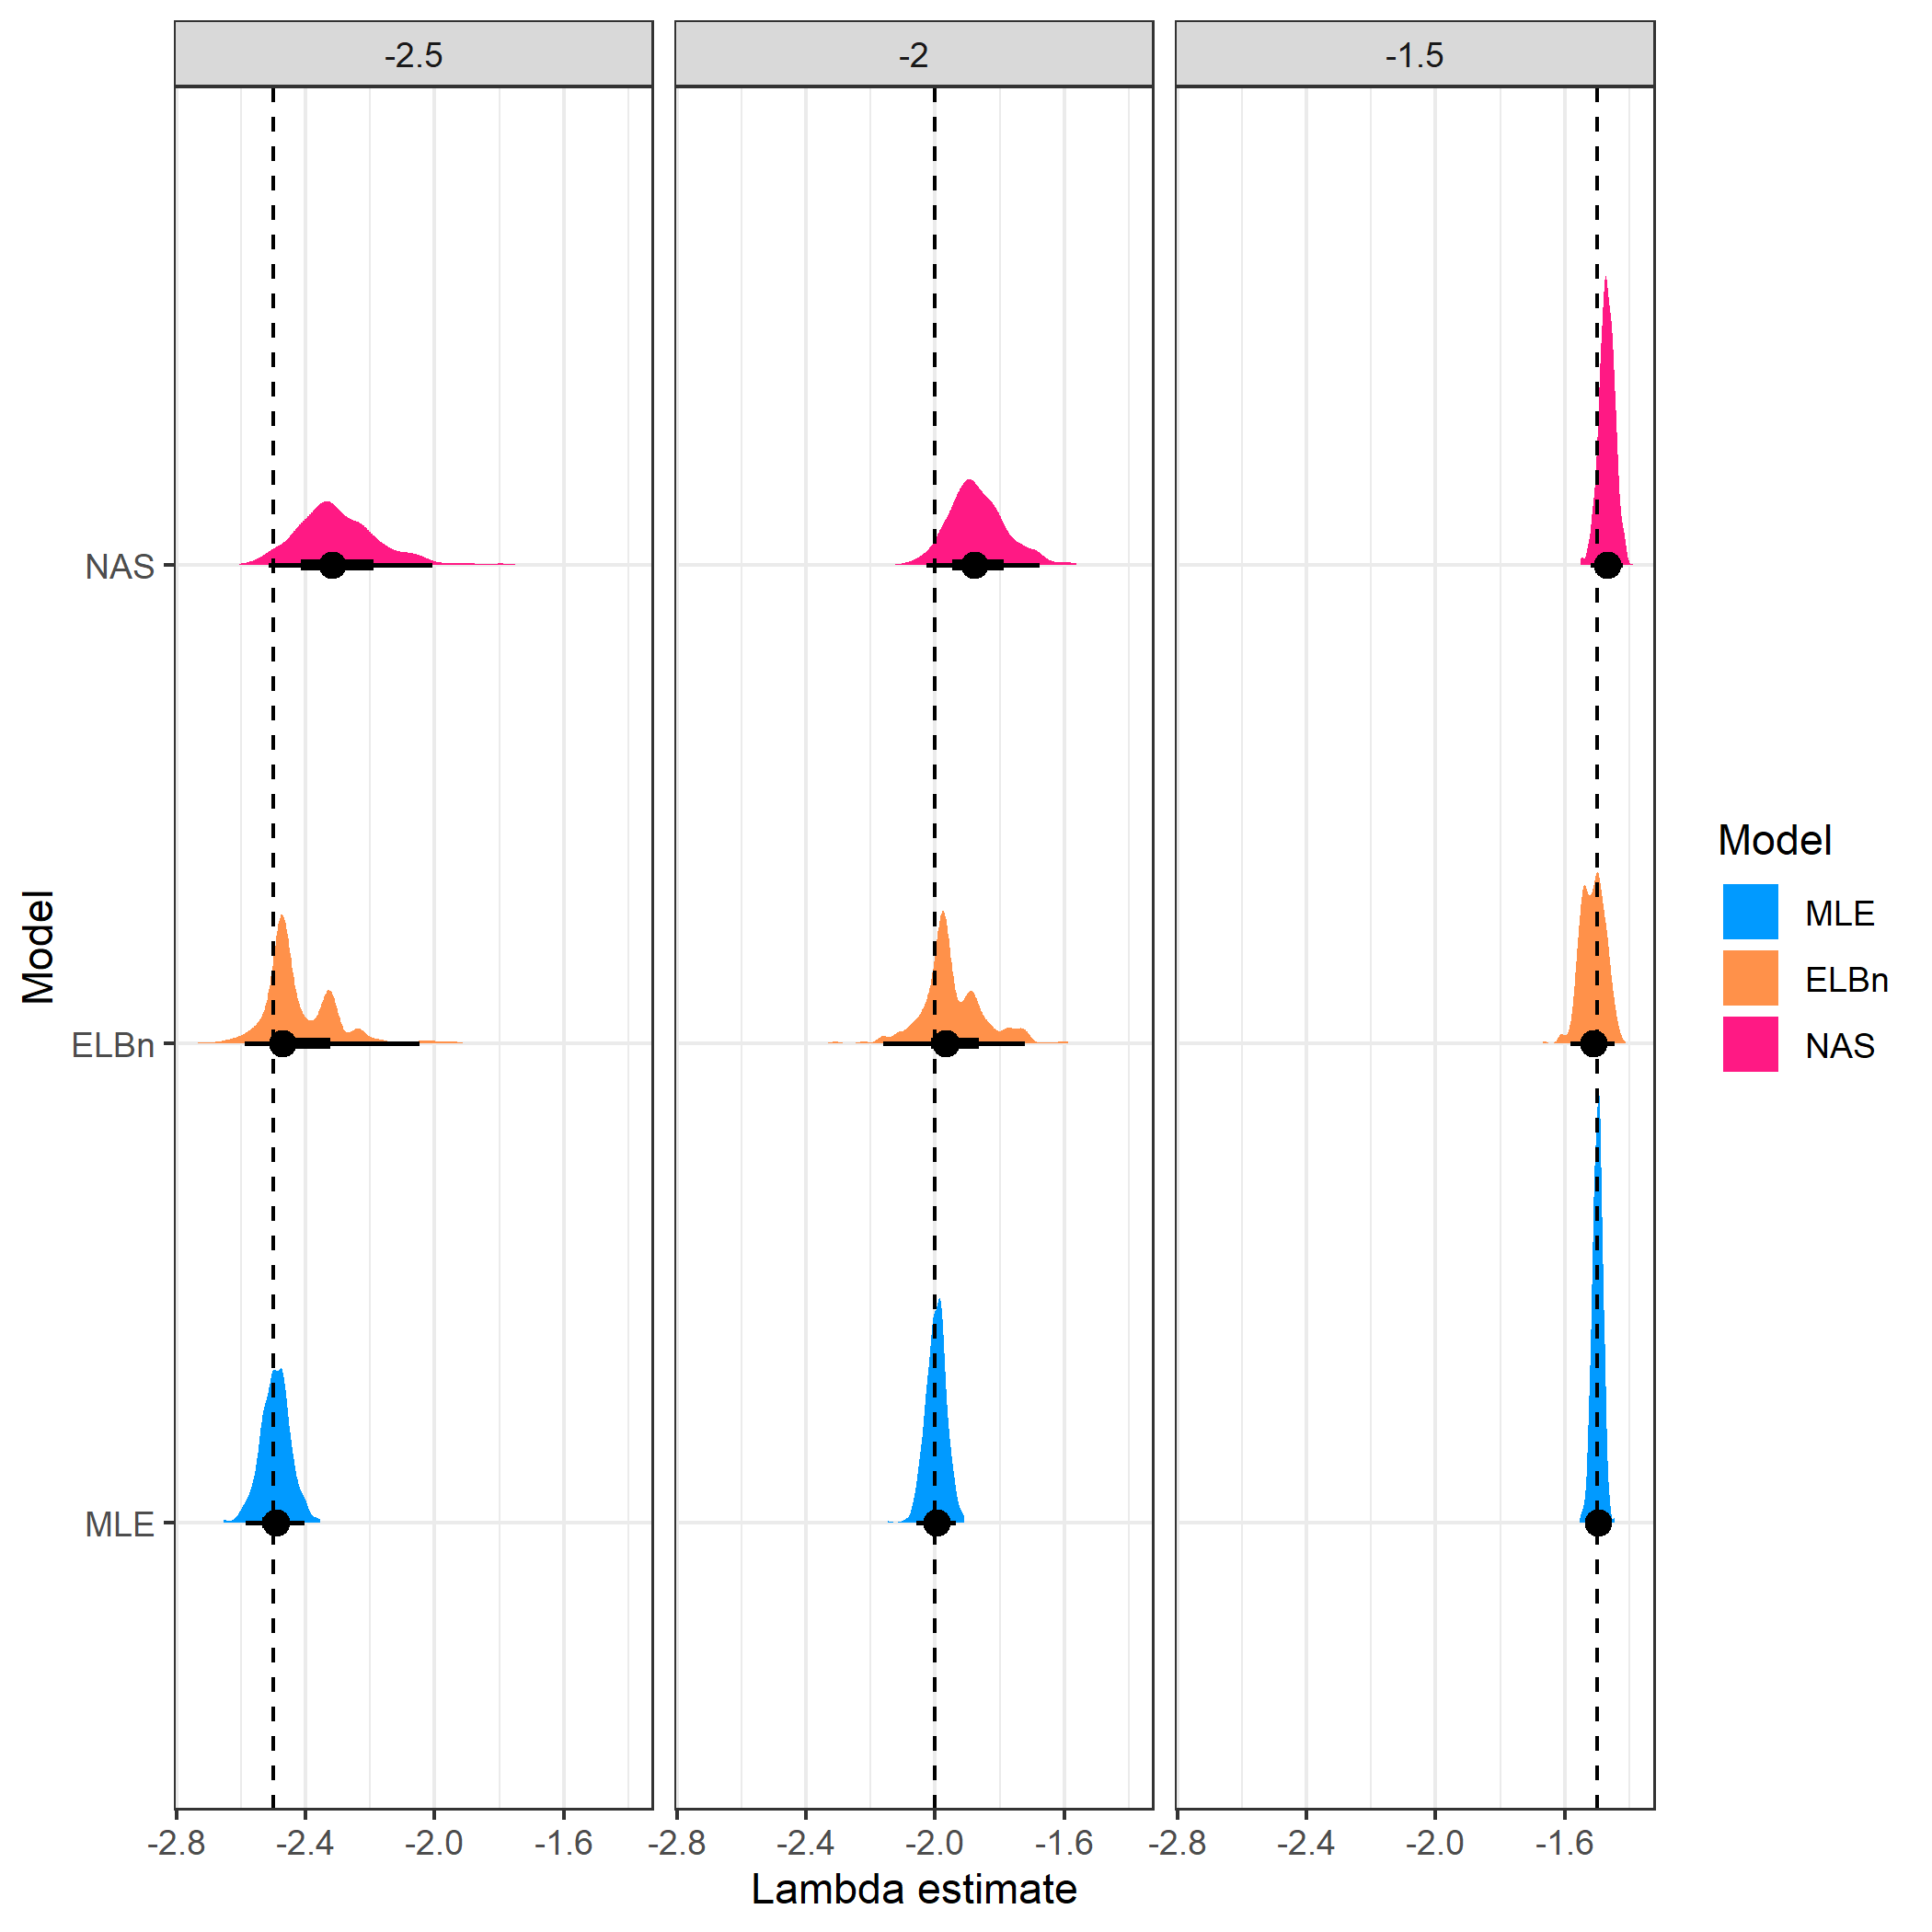
\includegraphics{figures/PLB_3_sites_est_b_density.png}
\caption{Distribution of estimated \(\lambda\) coefficient for three
sites across a hypothetical gradient with known values. All other
parameters are the same as in the main analysis.}
\end{figure}

\begin{figure}
\centering
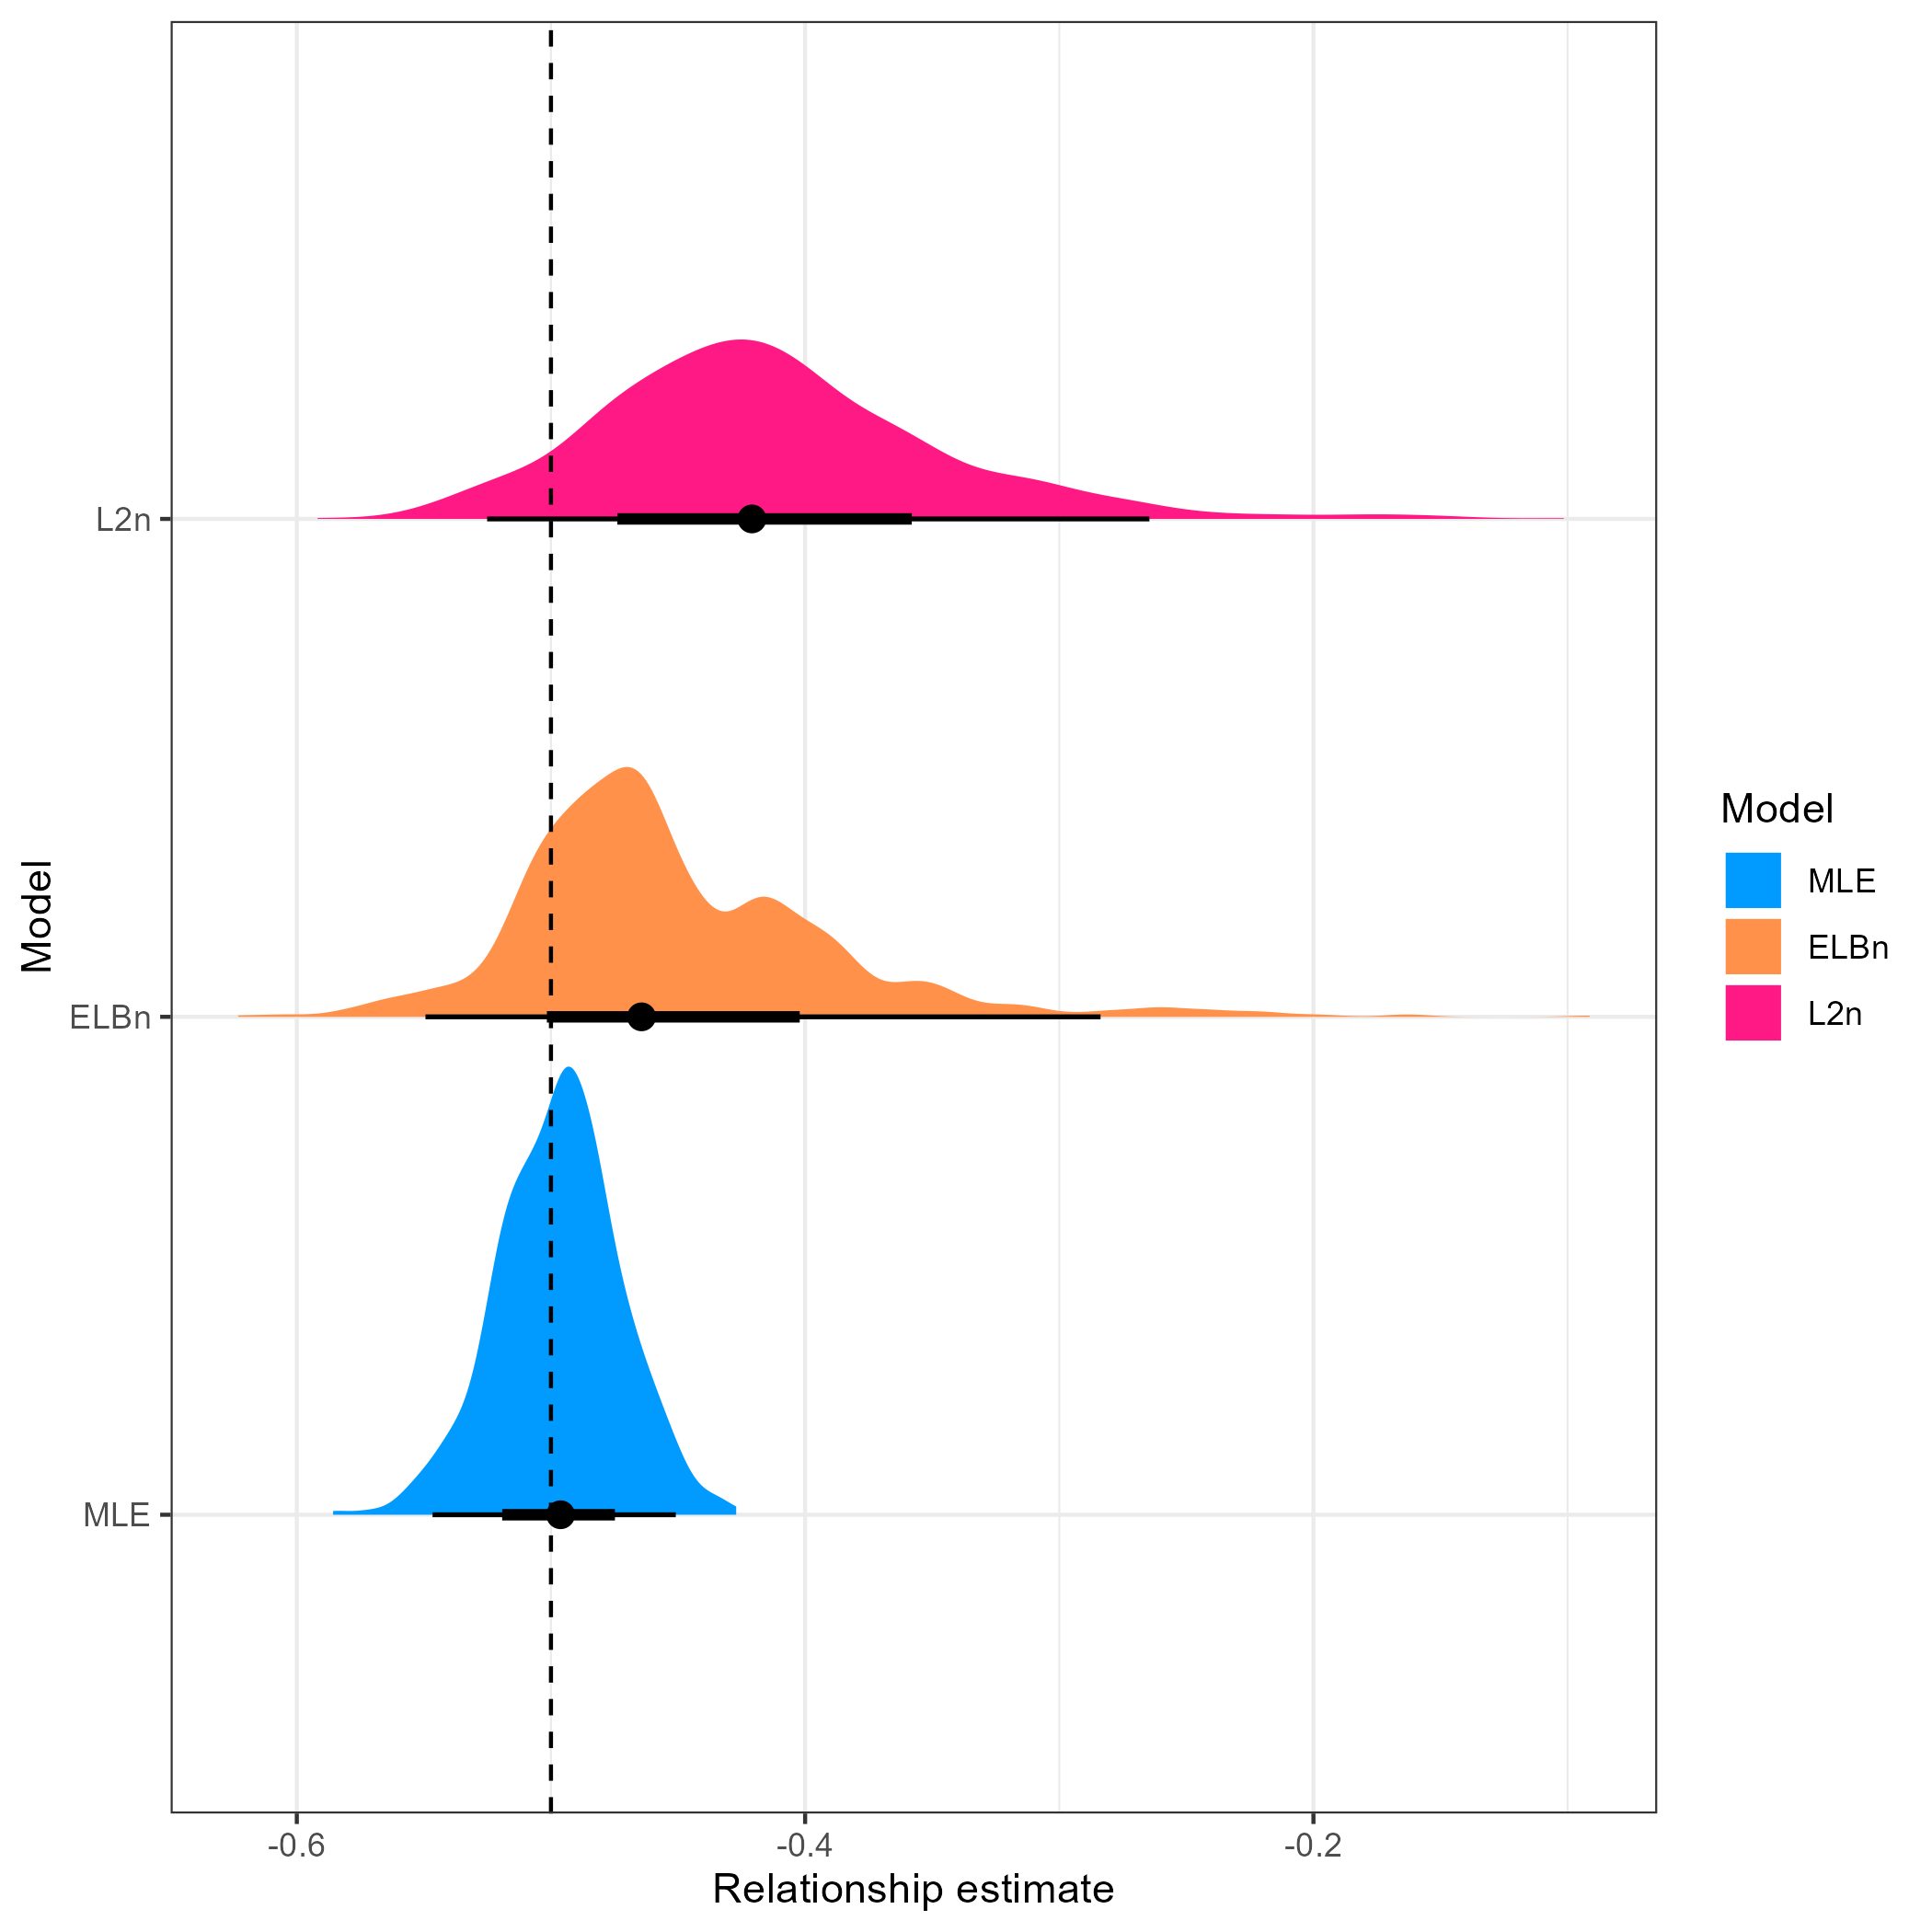
\includegraphics{figures/PLB_3_sites_relationship_density.png}
\caption{Distribution of estimated relationship (\(\beta_1\))
coefficient's for three sites across a hypothetical gradient with known
value of 0.5. All other parameters are the same as in the main analysis}
\end{figure}

\hypertarget{sample-size}{%
\subsection{Sample size}\label{sample-size}}

\textbf{note} These plots still have n = 100. Need to re run and update
if we end up going with n = 200

\begin{figure}
\centering
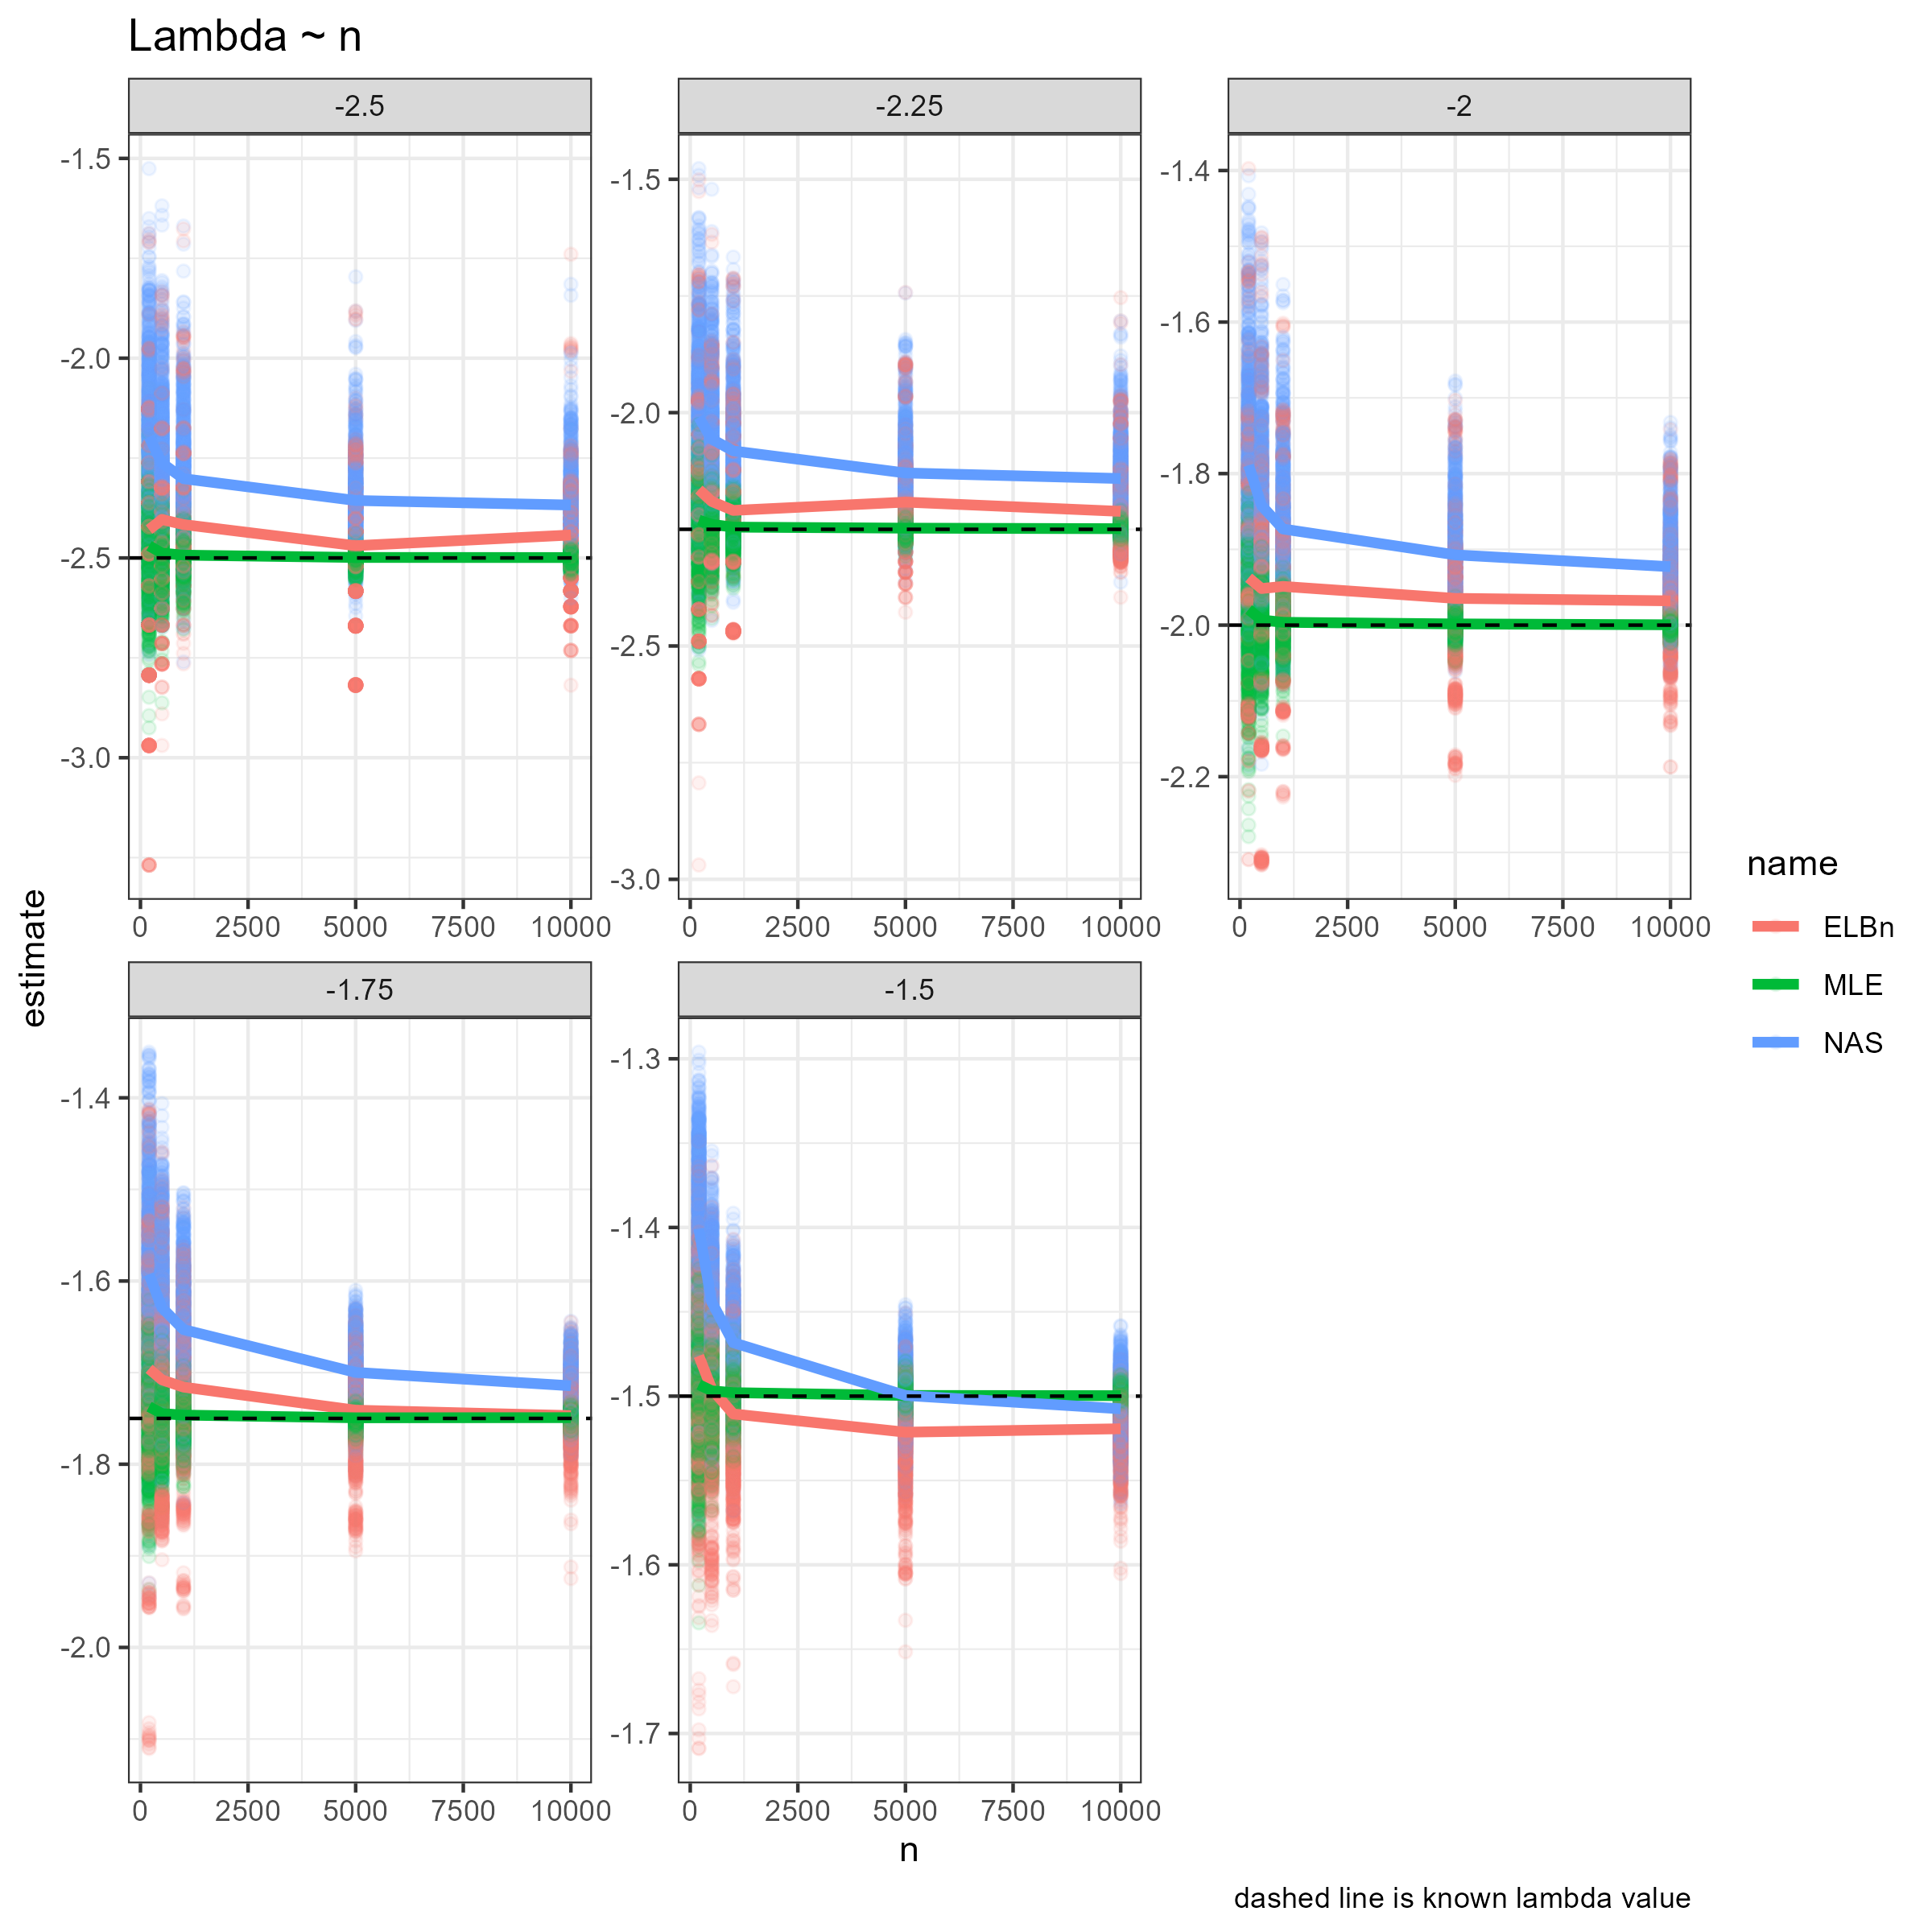
\includegraphics{figures/lambda_n_5_sites.png}
\caption{Plot showing the relationships between sample size and the
estimated \(\lambda\) parameters. the dashed line indicates the known
value of \(\lambda\).}
\end{figure}

\end{document}
